\documentclass[]{book}
\usepackage{lmodern}
\usepackage{amssymb,amsmath}
\usepackage{ifxetex,ifluatex}
\usepackage{fixltx2e} % provides \textsubscript
\ifnum 0\ifxetex 1\fi\ifluatex 1\fi=0 % if pdftex
  \usepackage[T1]{fontenc}
  \usepackage[utf8]{inputenc}
\else % if luatex or xelatex
  \ifxetex
    \usepackage{mathspec}
  \else
    \usepackage{fontspec}
  \fi
  \defaultfontfeatures{Ligatures=TeX,Scale=MatchLowercase}
\fi
% use upquote if available, for straight quotes in verbatim environments
\IfFileExists{upquote.sty}{\usepackage{upquote}}{}
% use microtype if available
\IfFileExists{microtype.sty}{%
\usepackage{microtype}
\UseMicrotypeSet[protrusion]{basicmath} % disable protrusion for tt fonts
}{}
\usepackage[margin=1in]{geometry}
\usepackage{hyperref}
\hypersetup{unicode=true,
            pdfborder={0 0 0},
            breaklinks=true}
\urlstyle{same}  % don't use monospace font for urls
\usepackage{natbib}
\bibliographystyle{apalike}
\usepackage{color}
\usepackage{fancyvrb}
\newcommand{\VerbBar}{|}
\newcommand{\VERB}{\Verb[commandchars=\\\{\}]}
\DefineVerbatimEnvironment{Highlighting}{Verbatim}{commandchars=\\\{\}}
% Add ',fontsize=\small' for more characters per line
\usepackage{framed}
\definecolor{shadecolor}{RGB}{248,248,248}
\newenvironment{Shaded}{\begin{snugshade}}{\end{snugshade}}
\newcommand{\AlertTok}[1]{\textcolor[rgb]{0.94,0.16,0.16}{#1}}
\newcommand{\AnnotationTok}[1]{\textcolor[rgb]{0.56,0.35,0.01}{\textbf{\textit{#1}}}}
\newcommand{\AttributeTok}[1]{\textcolor[rgb]{0.77,0.63,0.00}{#1}}
\newcommand{\BaseNTok}[1]{\textcolor[rgb]{0.00,0.00,0.81}{#1}}
\newcommand{\BuiltInTok}[1]{#1}
\newcommand{\CharTok}[1]{\textcolor[rgb]{0.31,0.60,0.02}{#1}}
\newcommand{\CommentTok}[1]{\textcolor[rgb]{0.56,0.35,0.01}{\textit{#1}}}
\newcommand{\CommentVarTok}[1]{\textcolor[rgb]{0.56,0.35,0.01}{\textbf{\textit{#1}}}}
\newcommand{\ConstantTok}[1]{\textcolor[rgb]{0.00,0.00,0.00}{#1}}
\newcommand{\ControlFlowTok}[1]{\textcolor[rgb]{0.13,0.29,0.53}{\textbf{#1}}}
\newcommand{\DataTypeTok}[1]{\textcolor[rgb]{0.13,0.29,0.53}{#1}}
\newcommand{\DecValTok}[1]{\textcolor[rgb]{0.00,0.00,0.81}{#1}}
\newcommand{\DocumentationTok}[1]{\textcolor[rgb]{0.56,0.35,0.01}{\textbf{\textit{#1}}}}
\newcommand{\ErrorTok}[1]{\textcolor[rgb]{0.64,0.00,0.00}{\textbf{#1}}}
\newcommand{\ExtensionTok}[1]{#1}
\newcommand{\FloatTok}[1]{\textcolor[rgb]{0.00,0.00,0.81}{#1}}
\newcommand{\FunctionTok}[1]{\textcolor[rgb]{0.00,0.00,0.00}{#1}}
\newcommand{\ImportTok}[1]{#1}
\newcommand{\InformationTok}[1]{\textcolor[rgb]{0.56,0.35,0.01}{\textbf{\textit{#1}}}}
\newcommand{\KeywordTok}[1]{\textcolor[rgb]{0.13,0.29,0.53}{\textbf{#1}}}
\newcommand{\NormalTok}[1]{#1}
\newcommand{\OperatorTok}[1]{\textcolor[rgb]{0.81,0.36,0.00}{\textbf{#1}}}
\newcommand{\OtherTok}[1]{\textcolor[rgb]{0.56,0.35,0.01}{#1}}
\newcommand{\PreprocessorTok}[1]{\textcolor[rgb]{0.56,0.35,0.01}{\textit{#1}}}
\newcommand{\RegionMarkerTok}[1]{#1}
\newcommand{\SpecialCharTok}[1]{\textcolor[rgb]{0.00,0.00,0.00}{#1}}
\newcommand{\SpecialStringTok}[1]{\textcolor[rgb]{0.31,0.60,0.02}{#1}}
\newcommand{\StringTok}[1]{\textcolor[rgb]{0.31,0.60,0.02}{#1}}
\newcommand{\VariableTok}[1]{\textcolor[rgb]{0.00,0.00,0.00}{#1}}
\newcommand{\VerbatimStringTok}[1]{\textcolor[rgb]{0.31,0.60,0.02}{#1}}
\newcommand{\WarningTok}[1]{\textcolor[rgb]{0.56,0.35,0.01}{\textbf{\textit{#1}}}}
\usepackage{longtable,booktabs}
\usepackage{graphicx,grffile}
\makeatletter
\def\maxwidth{\ifdim\Gin@nat@width>\linewidth\linewidth\else\Gin@nat@width\fi}
\def\maxheight{\ifdim\Gin@nat@height>\textheight\textheight\else\Gin@nat@height\fi}
\makeatother
% Scale images if necessary, so that they will not overflow the page
% margins by default, and it is still possible to overwrite the defaults
% using explicit options in \includegraphics[width, height, ...]{}
\setkeys{Gin}{width=\maxwidth,height=\maxheight,keepaspectratio}
\IfFileExists{parskip.sty}{%
\usepackage{parskip}
}{% else
\setlength{\parindent}{0pt}
\setlength{\parskip}{6pt plus 2pt minus 1pt}
}
\setlength{\emergencystretch}{3em}  % prevent overfull lines
\providecommand{\tightlist}{%
  \setlength{\itemsep}{0pt}\setlength{\parskip}{0pt}}
\setcounter{secnumdepth}{5}
% Redefines (sub)paragraphs to behave more like sections
\ifx\paragraph\undefined\else
\let\oldparagraph\paragraph
\renewcommand{\paragraph}[1]{\oldparagraph{#1}\mbox{}}
\fi
\ifx\subparagraph\undefined\else
\let\oldsubparagraph\subparagraph
\renewcommand{\subparagraph}[1]{\oldsubparagraph{#1}\mbox{}}
\fi

%%% Use protect on footnotes to avoid problems with footnotes in titles
\let\rmarkdownfootnote\footnote%
\def\footnote{\protect\rmarkdownfootnote}

%%% Change title format to be more compact
\usepackage{titling}

% Create subtitle command for use in maketitle
\newcommand{\subtitle}[1]{
  \posttitle{
    \begin{center}\large#1\end{center}
    }
}

\setlength{\droptitle}{-2em}

  \title{Single-Cell Data Integration using MINT}
    \pretitle{\vspace{\droptitle}\centering\huge}
  \posttitle{\par}
    \author{Al J Abadi, Dr Kim-Anh Lê Cao\\
~\\
Melbourne Integrative Genomics\\
The University of Melbourne}
    \preauthor{\centering\large\emph}
  \postauthor{\par}
      \predate{\centering\large\emph}
  \postdate{\par}
    \date{2018-11-14}

\usepackage{booktabs}

\usepackage{amsthm}
\newtheorem{theorem}{Theorem}[chapter]
\newtheorem{lemma}{Lemma}[chapter]
\theoremstyle{definition}
\newtheorem{definition}{Definition}[chapter]
\newtheorem{corollary}{Corollary}[chapter]
\newtheorem{proposition}{Proposition}[chapter]
\theoremstyle{definition}
\newtheorem{example}{Example}[chapter]
\theoremstyle{definition}
\newtheorem{exercise}{Exercise}[chapter]
\theoremstyle{remark}
\newtheorem*{remark}{Remark}
\newtheorem*{solution}{Solution}
\begin{document}
\maketitle

{
\setcounter{tocdepth}{1}
\tableofcontents
}
\hypertarget{how-to-reproduce-this-vignette}{%
\chapter{How to Reproduce this
Vignette}\label{how-to-reproduce-this-vignette}}

You need the `bookdown' package to reproduce this book. It is
recommended to clone the repository, open the .Rproj file and load the
Rmd files and create a `gitbook' from the `build' pane. You will also
need to open the '\_bookdown.yml' file using RStudio and remove the
argument: \emph{output\_dir: ``../docs''}.

Alternatively, you can run the standalone vignettes from the
\emph{vignettes-standalone} folder.

\begin{Shaded}
\begin{Highlighting}[]
\CommentTok{## install only if not installed}
\ControlFlowTok{if}\NormalTok{ (}\OperatorTok{!}\KeywordTok{requireNamespace}\NormalTok{(}\StringTok{'bookdown'}\NormalTok{, }\DataTypeTok{quietly =} \OtherTok{TRUE}\NormalTok{))\{}
  \KeywordTok{paste}\NormalTok{(}\StringTok{'Trying to install Bookdown'}\NormalTok{)}
  \KeywordTok{install.packages}\NormalTok{(}\StringTok{'bookdown'}\NormalTok{)}
\NormalTok{\}}
\end{Highlighting}
\end{Shaded}

\begin{Shaded}
\begin{Highlighting}[]
\CommentTok{## if loading the required input data locally}
\CommentTok{## input/output directories:}
\NormalTok{io =}\StringTok{ }\KeywordTok{list}\NormalTok{()}

\CommentTok{## SCE data dir - FALSE for GitHub load:}
\CommentTok{# io$local.sincell = '../data/sincell_with_class.RData'}
\NormalTok{io}\OperatorTok{$}\NormalTok{local.sincell =}\StringTok{ }\NormalTok{F }\CommentTok{# F or a directory}

\CommentTok{## where to save the run - FALSE for not saving:}
\CommentTok{# io$save.runs = '../output'}
\NormalTok{io}\OperatorTok{$}\NormalTok{save.runs =}\StringTok{ }\NormalTok{F }\CommentTok{# F or a directory}

\CommentTok{## where to save the R scripts - F for project directory:}
\CommentTok{# io$Rscript.dir = '../R-scripts'}
\NormalTok{io}\OperatorTok{$}\NormalTok{Rscript.dir =}\StringTok{ }\NormalTok{F}

\CommentTok{## save the final mint.splsda object in io$save.runs for signature analyses?:}
\NormalTok{io}\OperatorTok{$}\NormalTok{save.mint.spls =}\StringTok{ }\NormalTok{F }\CommentTok{# T or F}

\CommentTok{## DE tables directory for signature chapter - FALSE for GitHub load:}
\CommentTok{# io$DEtables = '../data/DEtable_90cells.RData'}
\NormalTok{io}\OperatorTok{$}\NormalTok{DEtables =}\StringTok{ }\NormalTok{F }\CommentTok{# F or a directory}
\end{Highlighting}
\end{Shaded}

\hypertarget{data-integration-with-mint}{%
\chapter{Data Integration with MINT}\label{data-integration-with-mint}}

This vignette explains the functionalities of \textbf{MINT}
(\textbf{M}ultivarite \textbf{INT}egrative method) \citep{mint} toolkit
in combining datasets from multiple single cell transcriptomic studies
on the same cell types. The integration is across the common \emph{P}
features. Hence, we call this framework \textbf{P-Integration}. We will
also illustrate why Prinicipal Component Analysis might not be as
powerful in such setting. It is worth mentioning that \emph{MINT} can be
used to combine datasets from any types of similar 'omics studies
(transcriptomics, proteomics, metabolomics, etc) on the samples which
share common features. For integration across different omics you can
use \href{http://mixomics.org/mixdiablo/}{DIABLO}.

\hypertarget{prerequisites}{%
\section{Prerequisites}\label{prerequisites}}

\emph{mixOmics} \citep{R-mixOmics} and the following Bioconductor/R
packages must be installed for this vignette:

\begin{Shaded}
\begin{Highlighting}[]
\CommentTok{## installing libraries}

\CommentTok{## installing BiocManager to install packages}
\CommentTok{## it can install CRAN packages as well}
\ControlFlowTok{if}\NormalTok{ (}\OperatorTok{!}\KeywordTok{requireNamespace}\NormalTok{(}\StringTok{'BiocManager'}\NormalTok{, }\DataTypeTok{quietly =} \OtherTok{TRUE}\NormalTok{))\{}
  \KeywordTok{paste}\NormalTok{(}\StringTok{'Trying to install BiocManager'}\NormalTok{)}
  \KeywordTok{install.packages}\NormalTok{(}\StringTok{'BiocManager'}\NormalTok{)}
\NormalTok{\}}

\CommentTok{## package installations (might take a bit of time)}
\NormalTok{BiocManager}\OperatorTok{::}\KeywordTok{install}\NormalTok{(}\StringTok{'mixOmics'}\NormalTok{, }\DataTypeTok{update =}\NormalTok{ F)}
\NormalTok{BiocManager}\OperatorTok{::}\KeywordTok{install}\NormalTok{(}\StringTok{'SingleCellExperiment'}\NormalTok{, }\DataTypeTok{update =}\NormalTok{ F) }\CommentTok{## single-cell experiment data analysis}
\NormalTok{BiocManager}\OperatorTok{::}\KeywordTok{install}\NormalTok{(}\StringTok{'scran'}\NormalTok{, }\DataTypeTok{update =}\NormalTok{ F) }\CommentTok{## sc-RNAseq data analysis}
\NormalTok{BiocManager}\OperatorTok{::}\KeywordTok{install}\NormalTok{(}\StringTok{'scater'}\NormalTok{, }\DataTypeTok{update =}\NormalTok{ F) }\CommentTok{## sc gene expression analysis}
\NormalTok{BiocManager}\OperatorTok{::}\KeywordTok{install}\NormalTok{(}\StringTok{'vennDiagram'}\NormalTok{, }\DataTypeTok{update =}\NormalTok{ F) }\CommentTok{## Venn diagrams}
\NormalTok{BiocManager}\OperatorTok{::}\KeywordTok{install}\NormalTok{(}\StringTok{'tibble'}\NormalTok{, }\DataTypeTok{update =}\NormalTok{ F) }\CommentTok{## for data tables}
\end{Highlighting}
\end{Shaded}

If any issues arise during package installations, you can check out the
\protect\hyperlink{troubleshoots}{Troubleshoots} section.

\hypertarget{why-mint}{%
\section{Why MINT?}\label{why-mint}}

Different datasets often contain different levels of unwanted variation
that come from factors other than biology of study (e.g.~differences in
the technology, protocol, etc.) known as batch effects. The \emph{MINT}
framework presented in this vignette is an integrative method that helps
to find the common structures in the combined dataset which best explain
their biological class membership (cell type), and thus can potentially
lead us to insightful signatures. For further examples on bulk data, you
can also check out a case study on
\href{http://mixomics.org/mixmint/stemcells-example/}{mixOmics'
website}.

\hypertarget{when-not-to-use-mint}{%
\section{When Not to Use MINT?}\label{when-not-to-use-mint}}

Current version of \emph{MINT} performs supervised data integration.
Therefore, the phenotypes/cell types must be known prior to data
integration using this method.

\hypertarget{r-scripts}{%
\section{R scripts}\label{r-scripts}}

The R scripts are available at
\href{https://github.com/AJABADI/MINT_sPLSDA/blob/master/01-Data-Integration.R}{this
link}.

\hypertarget{libraries}{%
\section{Libraries}\label{libraries}}

Here we load the libraries installed in
\protect\hyperlink{prerequisites}{Prerequisites}:

\begin{Shaded}
\begin{Highlighting}[]
\CommentTok{## load the required libraries}
\KeywordTok{library}\NormalTok{(SingleCellExperiment)}
\KeywordTok{library}\NormalTok{(mixOmics)}
\KeywordTok{library}\NormalTok{(scran)}
\KeywordTok{library}\NormalTok{(scater)}
\KeywordTok{library}\NormalTok{(knitr)}
\KeywordTok{library}\NormalTok{(VennDiagram)}
\KeywordTok{library}\NormalTok{(tibble)}
\end{Highlighting}
\end{Shaded}

\hypertarget{data}{%
\section{Data}\label{data}}

The benchmark data - available on
\href{https://github.com/LuyiTian/CellBench_data}{github} - were
obtained from our collaborators Luyi Tian and Dr Matt Ritchie at WEHI.
Briefly, cells from three human cell lines H2228, H1975, HCC827
collected on lung tissue (Adenocarcinoma; Non-Small Cell Lung Cancer)
were barcoded and pooled in equal amounts. The samples were then
processed through three different types of 3' end sequencing protocols
that span the range of isolation strategies available:

\begin{itemize}
\tightlist
\item
  Droplet-based capture with:

  \begin{itemize}
  \tightlist
  \item
    Chromium 10X (10X Genomics)
  \item
    Drop-seq (Dolomite).
  \end{itemize}
\item
  Plate based isolation of cells in microwells with CEL-seq2.
\end{itemize}

Therefore, in addition to the biological variability coming from three
distinct and separately cultured cell lines, the datasets are likely to
also contain different layers of technical variability coming from three
sequencing protocols and technologies.

\begin{figure}[ht]

{\centering 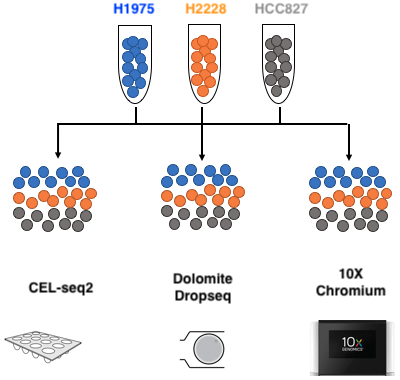
\includegraphics[width=0.45\linewidth]{figures/exp_design3} 

}

\caption{Benchmark experiment design: mixture of the three pure cells in equal proportion, processed through 3 different sequencing technologies. Adopted from Luyi Tian slides.}\label{fig:1-Experimental-Design}
\end{figure}

Throughout this vignette, the terms \emph{batch}, \emph{protocol}, and
\emph{study} are used interchangeably.

\hypertarget{loading-the-data}{%
\section{Loading the Data}\label{loading-the-data}}

We load the data directly from the
\href{https://github.com/LuyiTian/CellBench_data/tree/master/data}{github
repository} into R environment:

\begin{Shaded}
\begin{Highlighting}[]
\CommentTok{## load from github}
\NormalTok{DataURL=}\StringTok{'https://tinyurl.com/sincell-with-class-RData-LuyiT'}
\KeywordTok{load}\NormalTok{(}\KeywordTok{url}\NormalTok{(DataURL))}
\end{Highlighting}
\end{Shaded}

But you can download and load them from your working directory as well
(you must download the \emph{sincell\_with\_class.RData} file from the
repository):

\textbf{Tip}: For convenience, throughout the runs you may also want to
save the finalised RData file from each section using the \emph{save}
function for easy loading using \emph{load} function in the downstream
analyses (refer to R documentation for more details).

The loaded datasets consist of:

\begin{itemize}
\tightlist
\item
  \emph{sce10x\_qc}: From the Chromium 10X technology;
\item
  \emph{sce4\_qc}: From the CEL-seq2 technology; and
\item
  \emph{scedrop\_qc\_qc}: From the Drop-seq technology (quality
  controlled twice due to abundant outliers).
\end{itemize}

Each dataset is of \emph{SingleCellExperiment (SCE)} class, which is an
extension of the
\href{https://www.rdocumentation.org/packages/SummarizedExperiment/versions/1.2.3/topics/RangedSummarizedExperiment-class}{\emph{RangedSummarizedExperiment}}
class. For more details see the
\href{https://bioconductor.org/packages/devel/bioc/vignettes/SingleCellExperiment/inst/doc/intro.html}{package's
vignette} or refer to the R Documentation.

\hypertarget{quality-control}{%
\subsection{Quality Control}\label{quality-control}}

The data have been quality controlled using
\href{https://bioconductor.org/packages/release/bioc/html/scPipe.html}{\emph{scPipe}
package}. It is a Bioconductor package that can handle data generated
from all 64 popular 3' end scRNA-seq protocols and their variants
\citep{R-scPipe}.

\hypertarget{overview}{%
\subsection{Overview}\label{overview}}

we now stratify the cell and gene data by cell line in each protocol.

\begin{Shaded}
\begin{Highlighting}[]
\CommentTok{## make a summary of QC'ed cell line data processed by each protocol}
\NormalTok{sce10xqc_smr =}\StringTok{  }\KeywordTok{summary}\NormalTok{(}\KeywordTok{as.factor}\NormalTok{(sce10x_qc}\OperatorTok{$}\NormalTok{cell_line))}
\NormalTok{sce4qc_smr =}\StringTok{    }\KeywordTok{summary}\NormalTok{(}\KeywordTok{as.factor}\NormalTok{(sce4_qc}\OperatorTok{$}\NormalTok{cell_line))}
\NormalTok{scedropqc_smr =}\StringTok{ }\KeywordTok{summary}\NormalTok{(}\KeywordTok{as.factor}\NormalTok{(scedrop_qc_qc}\OperatorTok{$}\NormalTok{cell_line))}
\CommentTok{## combine the summaries}
\NormalTok{celline_smr =}\StringTok{ }\KeywordTok{rbind}\NormalTok{(sce10xqc_smr,sce4qc_smr,scedropqc_smr)}
\CommentTok{## produce a 'total' row as well}
\NormalTok{celline_smr =}\StringTok{ }\KeywordTok{cbind}\NormalTok{(celline_smr, }\KeywordTok{apply}\NormalTok{(celline_smr,}\DecValTok{1}\NormalTok{,sum))}
\CommentTok{## add the genes as well}
\NormalTok{celline_smr =}\StringTok{ }\KeywordTok{cbind}\NormalTok{(celline_smr,}
                    \KeywordTok{c}\NormalTok{(}\KeywordTok{dim}\NormalTok{(}\KeywordTok{counts}\NormalTok{(sce10x_qc))[}\DecValTok{1}\NormalTok{],}
                      \KeywordTok{dim}\NormalTok{(}\KeywordTok{counts}\NormalTok{(sce4_qc))[}\DecValTok{1}\NormalTok{],}
                      \KeywordTok{dim}\NormalTok{(}\KeywordTok{counts}\NormalTok{(scedrop_qc_qc))[}\DecValTok{1}\NormalTok{]))}
\CommentTok{## label the rows}
\KeywordTok{row.names}\NormalTok{(celline_smr) =}\StringTok{ }\KeywordTok{c}\NormalTok{(}\StringTok{'10X'}\NormalTok{, }\StringTok{'CEL-seq2'}\NormalTok{, }\StringTok{'Drop-seq'}\NormalTok{)}
\KeywordTok{colnames}\NormalTok{(celline_smr) =}\StringTok{ }\KeywordTok{c}\NormalTok{(}\StringTok{'H1975'}\NormalTok{, }\StringTok{'H2228'}\NormalTok{, }\StringTok{'HCC827'}\NormalTok{, }
                          \StringTok{'Total Cells'}\NormalTok{,}\StringTok{'Total Genes'}\NormalTok{)}
\end{Highlighting}
\end{Shaded}

\begin{Shaded}
\begin{Highlighting}[]
\CommentTok{## tabulate the summaries}
\KeywordTok{kable}\NormalTok{(celline_smr,}
      \DataTypeTok{caption =} \StringTok{'Summary of cell and gene data }
\StringTok{      per cell line for each protocol'}\NormalTok{)}
\end{Highlighting}
\end{Shaded}

\begin{table}

\caption{\label{tab:1-summaryKable}Summary of cell and gene data 
      per cell line for each protocol}
\centering
\begin{tabular}[t]{l|r|r|r|r|r}
\hline
  & H1975 & H2228 & HCC827 & Total Cells & Total Genes\\
\hline
10X & 313 & 315 & 274 & 902 & 16468\\
\hline
CEL-seq2 & 114 & 81 & 79 & 274 & 28204\\
\hline
Drop-seq & 92 & 65 & 68 & 225 & 15127\\
\hline
\end{tabular}
\end{table}

The assignment to each cell line was performed computationally based on
the correlation of the gene expression data with a bulk assay of a
mixture of cells by DE analysis using
\href{https://bioconductor.org/packages/release/bioc/html/edgeR.html}{\emph{edgeR}}.

The 10X protocol yielded the highest number of cellls
(\textasciitilde{}900). We can visualise the the total amount of genes
in each protocol and the amount of overlapping genes among the protocols
using a venn diagram:

\begin{Shaded}
\begin{Highlighting}[]
\CommentTok{## create venn diagram of genes in each protocol:}
\NormalTok{venn.plot =}\StringTok{ }\KeywordTok{venn.diagram}\NormalTok{(}
  \DataTypeTok{x =} \KeywordTok{list}\NormalTok{(}\DataTypeTok{Chrom.10X =} \KeywordTok{rownames}\NormalTok{(sce10x_qc),}
           \DataTypeTok{CEL.seq2 =} \KeywordTok{rownames}\NormalTok{(sce4_qc),}
           \DataTypeTok{Drop.seq =} \KeywordTok{rownames}\NormalTok{(scedrop_qc_qc)),}
  \DataTypeTok{filename =} \OtherTok{NULL}\NormalTok{, }\DataTypeTok{label=}\OtherTok{TRUE}\NormalTok{, }\DataTypeTok{margin=}\FloatTok{0.05}\NormalTok{,}
  \DataTypeTok{height =} \DecValTok{1400}\NormalTok{, }\DataTypeTok{width =} \DecValTok{2200}\NormalTok{,}
  \DataTypeTok{col =} \StringTok{'transparent'}\NormalTok{, }\DataTypeTok{fill =} \KeywordTok{c}\NormalTok{(}\StringTok{'cornflowerblue'}\NormalTok{,}\StringTok{'green'}\NormalTok{, }\StringTok{'red'}\NormalTok{),}
  \DataTypeTok{alpha =} \FloatTok{0.60}\NormalTok{, }\DataTypeTok{cex =} \DecValTok{2}\NormalTok{, }\DataTypeTok{fontfamily =} \StringTok{'serif'}\NormalTok{, }\DataTypeTok{fontface =} \StringTok{'bold'}\NormalTok{,}
  \DataTypeTok{cat.col =} \KeywordTok{c}\NormalTok{(}\StringTok{'darkblue'}\NormalTok{, }\StringTok{'darkgreen'}\NormalTok{, }\StringTok{'black'}\NormalTok{), }\DataTypeTok{cat.cex =} \FloatTok{2.2}\NormalTok{)}

\CommentTok{## save the plot, change to your own directory}
\KeywordTok{png}\NormalTok{(}\DataTypeTok{filename =} \StringTok{'figures/GeneVenn.png'}\NormalTok{)}
\KeywordTok{grid.draw}\NormalTok{(venn.plot)}
\KeywordTok{dev.off}\NormalTok{()}
\end{Highlighting}
\end{Shaded}

\begin{figure}[ht]

{\centering 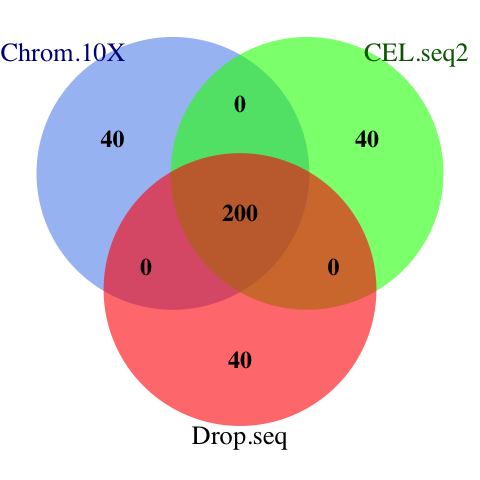
\includegraphics[width=0.4\linewidth]{figures/GeneVenn} 

}

\caption{ The venn diagram of common genes among datasets. MINT uses the common features of all datasets for discriminant analysis.}\label{fig:1-vennDiag}
\end{figure}

A total of 13757 genes are shared across three datasets.

\hypertarget{normalisation}{%
\subsection{Normalisation}\label{normalisation}}

Normalisation is typically required in RNA-seq data analysis prior to
downstream analysis to reduce heterogeneity among samples due to
technical artefact as well as to help to impute the missing values using
known data.

We use the
\href{http://bioconductor.org/packages/release/bioc/html/scran.html}{\emph{scran}
package}'s ``Normalisation by deconvolution of size factors from cell
pools'' method \citep{scnorm}. It is a two-step process, in which the
size factors are adjusted, and then the expression values are
normalised:

\begin{Shaded}
\begin{Highlighting}[]
\CommentTok{## normalise the QC'ed count matrices}
\NormalTok{sc10x.norm =}\StringTok{  }\KeywordTok{computeSumFactors}\NormalTok{(sce10x_qc) }\CommentTok{## deconvolute using size factors}
\NormalTok{sc10x.norm =}\StringTok{  }\KeywordTok{normalize}\NormalTok{(sc10x.norm) }\CommentTok{## normalise expression values}
\CommentTok{## DROP-seq}
\NormalTok{scdrop.norm =}\StringTok{ }\KeywordTok{computeSumFactors}\NormalTok{(scedrop_qc_qc)}
\NormalTok{scdrop.norm =}\StringTok{ }\KeywordTok{normalize}\NormalTok{(scdrop.norm)}
\CommentTok{## CEL-seq2}
\NormalTok{sccel.norm =}\StringTok{  }\KeywordTok{computeSumFactors}\NormalTok{(sce4_qc)}
\NormalTok{sccel.norm =}\StringTok{  }\KeywordTok{normalize}\NormalTok{(sccel.norm)}
\end{Highlighting}
\end{Shaded}

Depending on the data structure and/or the question in hand the
following analyses can have one of the following two forms:

\begin{itemize}
\item
  \textbf{Unsupervised Analysis:} Where we want to explore the patterns
  among the data and find the main directions that drive the variations
  in the dataset. \textbf{It is often beneficial to perform unsupervised
  analysis prior to supervised analysis to assess the presence of
  outliers and/or batch effects}.
\item
  \textbf{Supervised Analysis:} In which each sample consists of a pair
  of feature measurements (e.g.~gene counts) and class membership
  (e.g.~cell type). The aim is to build a model that maps the
  measurements to their classes using a training set which can
  adequately predict classes in a test set as well.
\end{itemize}

We will start with Unsupervised Analysis and then proceed to Supervised
Analysis.

\hypertarget{pca-unsupervised-analysis}{%
\section{PCA: Unsupervised Analysis}\label{pca-unsupervised-analysis}}

We start by Principal Component Analysis (PCA) \citep{pca}. It is a
dimension reduction method which seeks for components that maximise the
variance within the datasets. PCA is primarily used to explore one
single type of `omics data (e.g.~transcriptomics, proteomics,
metabolomics data, etc). It is an unsupervised learning method and thus
there is no assumption of data corresponding to any class (batch, study
etc).

\begin{figure}[ht]

{\centering 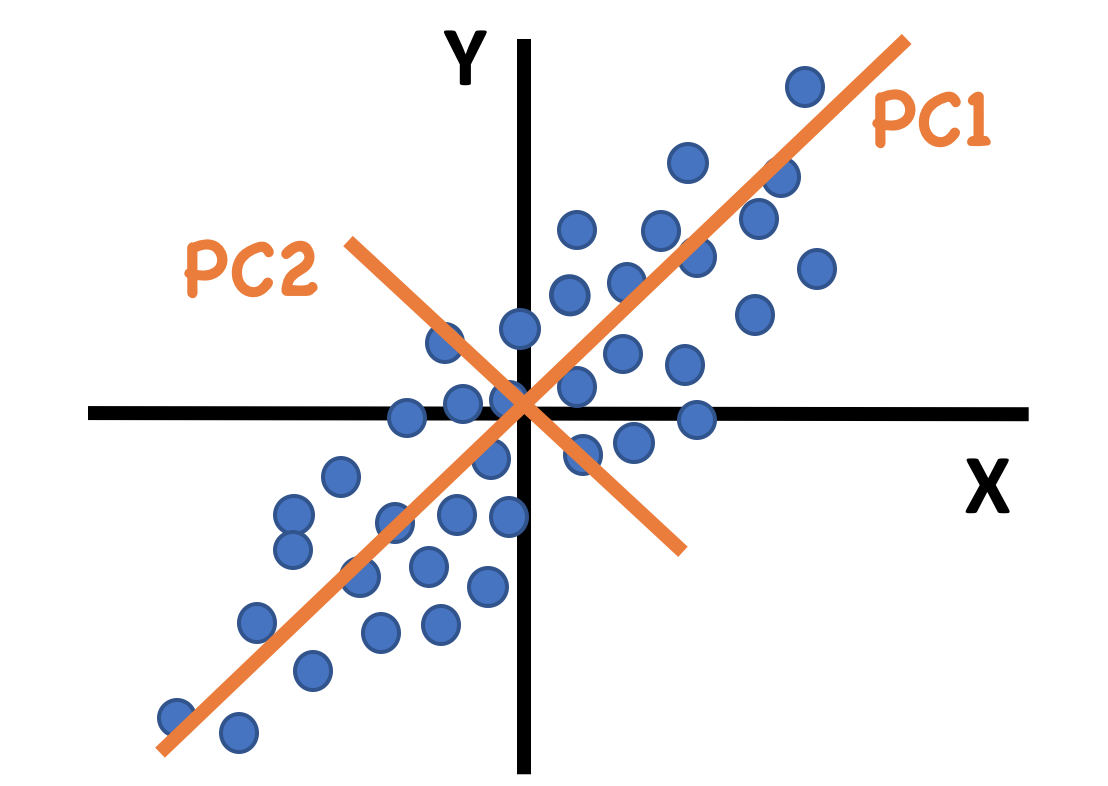
\includegraphics[width=0.4\linewidth]{figures/pca} 

}

\caption{An example of principal components for data with only 2 dimensions. The first PC is along the direction of maximum variance.}\label{fig:1-pcaExample}
\end{figure}

The first Principal Component (PC) explains as much variance in the data
as possible, and each following PC explains as much of the remaining
variance as possible, in a direction orthogonal to all previous PCs.
Thus, the first few components often capture the main variance in a
dataset.

We will perform PCA on the datasets from each protocol separately and
then conduct a PCA on the concatenated dataset.

\hypertarget{pca-on-each-protocol-individually}{%
\subsection{PCA on Each Protocol
Individually}\label{pca-on-each-protocol-individually}}

We will use \emph{mixOmics}'s \emph{pca} function in this section. The
method is implemented numerically and it is capable of dealing with
datasets with or without missing values (see documentation for details).
The \emph{pca} function takes the data as a matrix of count data.
Contrary to conventional biological data formation, \emph{pca} takes
each row to be the gene expression profile of a molecule/cell.
Therefore, we will have to transpose the normalised matrix (using the
\emph{t()} function) to perform PCA. Additionally, we use the log
transformed counts (\emph{logcounts()}) to confine the counts' span for
numerical reasons.

By default, \emph{mixOmics} centres the normalised matrix to have zero
mean. The \emph{scale} argument can also be set to `TRUE' if there are
diverse units in raw data.

The \emph{ncomp} argument denotes the number of desired PCs to
find\footnote{More arguments: \emph{max.iter, tol, logratio,
  multilevel}.}. We will retrieve 10 PCs for each protocol at this
stage:

\begin{Shaded}
\begin{Highlighting}[]
\CommentTok{## pca on the normlaised count matrices and find 10 PCs}
\NormalTok{pca.res}\FloatTok{.10}\NormalTok{x =}\StringTok{     }\KeywordTok{pca}\NormalTok{(}\KeywordTok{t}\NormalTok{(}\KeywordTok{logcounts}\NormalTok{(sc10x.norm)),  }\DataTypeTok{ncomp =} \DecValTok{10}\NormalTok{,}
                      \DataTypeTok{center=}\OtherTok{TRUE}\NormalTok{, }\DataTypeTok{scale=}\OtherTok{FALSE}\NormalTok{)}
\NormalTok{pca.res.celseq =}\StringTok{  }\KeywordTok{pca}\NormalTok{(}\KeywordTok{t}\NormalTok{(}\KeywordTok{logcounts}\NormalTok{(sccel.norm)),  }\DataTypeTok{ncomp =} \DecValTok{10}\NormalTok{,}
                      \DataTypeTok{center=}\OtherTok{TRUE}\NormalTok{, }\DataTypeTok{scale=}\OtherTok{FALSE}\NormalTok{)}
\NormalTok{pca.res.dropseq =}\StringTok{ }\KeywordTok{pca}\NormalTok{(}\KeywordTok{t}\NormalTok{(}\KeywordTok{logcounts}\NormalTok{(scdrop.norm)), }\DataTypeTok{ncomp =} \DecValTok{10}\NormalTok{,}
                      \DataTypeTok{center=}\OtherTok{TRUE}\NormalTok{, }\DataTypeTok{scale=}\OtherTok{FALSE}\NormalTok{)}
\end{Highlighting}
\end{Shaded}

Each output is a \emph{pca} object that includes the centred count
matrix for that protocol, the mean normalised counts for each gene, the
PCA loadings, and score values.

It is possible to use the \emph{plot} function on \emph{pca} object to
visualise the proportion of the total variance of the data explained by
each of the 10 PCs for each protocol using a barplot:

\begin{Shaded}
\begin{Highlighting}[]
\CommentTok{## arrange the plots in 1 row and 3 columns}
\KeywordTok{par}\NormalTok{(}\DataTypeTok{mfrow=}\KeywordTok{c}\NormalTok{(}\DecValTok{1}\NormalTok{,}\DecValTok{3}\NormalTok{))}
\CommentTok{## find the maximum explained variance in all PCs:}
\NormalTok{ymax =}\StringTok{ }\KeywordTok{max}\NormalTok{ (pca.res}\FloatTok{.10}\NormalTok{x}\OperatorTok{$}\NormalTok{explained_variance[}\DecValTok{1}\NormalTok{],}
\NormalTok{             pca.res.celseq}\OperatorTok{$}\NormalTok{explained_variance[}\DecValTok{1}\NormalTok{],}
\NormalTok{             pca.res.dropseq}\OperatorTok{$}\NormalTok{explained_variance[}\DecValTok{1}\NormalTok{])}

\CommentTok{## plot the pca objects and limit the Y axes to ymax for all}
\KeywordTok{plot}\NormalTok{(pca.res}\FloatTok{.10}\NormalTok{x, }\DataTypeTok{main=} \StringTok{'(A) 10X'}\NormalTok{, }\DataTypeTok{ylim=}\KeywordTok{c}\NormalTok{(}\DecValTok{0}\NormalTok{,ymax))}
\KeywordTok{plot}\NormalTok{(pca.res.celseq,  }\DataTypeTok{main=} \StringTok{'(B) CEL-seq2'}\NormalTok{, }\DataTypeTok{ylim=}\KeywordTok{c}\NormalTok{(}\DecValTok{0}\NormalTok{,ymax))}
\KeywordTok{plot}\NormalTok{(pca.res.dropseq,  }\DataTypeTok{main=} \StringTok{'(C) Drop-seq'}\NormalTok{, }\DataTypeTok{ylim=}\KeywordTok{c}\NormalTok{(}\DecValTok{0}\NormalTok{,ymax))}
\end{Highlighting}
\end{Shaded}

\begin{figure}[ht]

{\centering 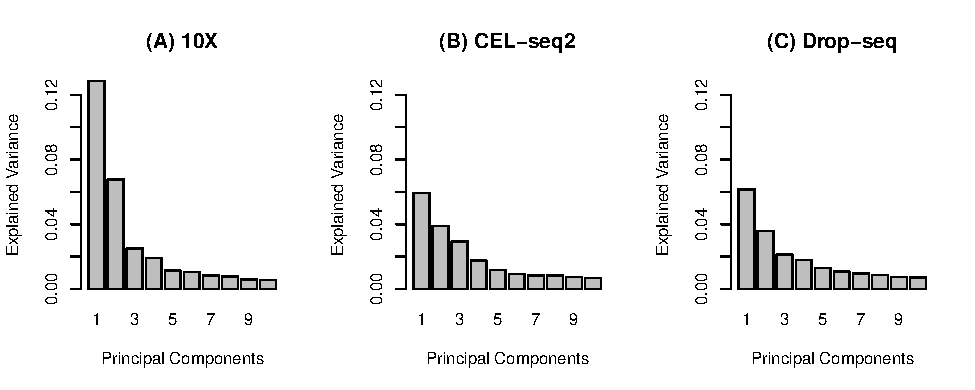
\includegraphics[width=1\linewidth]{MINT_Data_Integration_files/figure-latex/1-screeplots-1} 

}

\caption{The pca barplot for each protocol. (A) The first 2 PCs explain 20\% of total variability of the data and there is a drop (elbow) in the explained variability afterwards. (B) The first 2 PCs explain 10\% of variability and an elbow is not apparent. (C) similar cumulative explained variance to CEL-seq2 for first 2 PCs.}\label{fig:1-screeplots}
\end{figure}

It will usually be desirable if the first few PCs capture sufficient
variation in the data, as this will help with visualisation.

In order to have a simple 2D scatter plot, the first 2 PCs are usually
the ones of interest in PCA plots\footnote{Using the ``style=`3d'\,''
  argument, one can also plot the 3d PCA plot with 3 components}. Such a
plot can be created using the \emph{plotIndiv} function. For a complete
list of the argument options refer to the documentation.

We will colour the data points of each cell line using \emph{group}
argument to see whether there is a differentiation between different
cell types:

\begin{Shaded}
\begin{Highlighting}[]
\CommentTok{## define custom colours/shapes}
\CommentTok{## colour by cell line}
\NormalTok{col.cell =}\StringTok{ }\KeywordTok{c}\NormalTok{(}\StringTok{'H1975'}\NormalTok{=}\StringTok{'#0000ff'}\NormalTok{, }\StringTok{'HCC827'}\NormalTok{=}\StringTok{'grey30'}\NormalTok{, }\StringTok{'H2228'}\NormalTok{ =}\StringTok{'#ff8000'}\NormalTok{)}
\CommentTok{## shape by batch}
\NormalTok{shape.batch =}\StringTok{ }\KeywordTok{c}\NormalTok{(}\StringTok{'10X'}\NormalTok{ =}\StringTok{ }\DecValTok{1}\NormalTok{, }\StringTok{'CEL-seq2'}\NormalTok{=}\DecValTok{2}\NormalTok{, }\StringTok{'Drop-seq'}\NormalTok{=}\DecValTok{3}\NormalTok{ )}
\end{Highlighting}
\end{Shaded}

\begin{Shaded}
\begin{Highlighting}[]
\CommentTok{## pca plots for protocols}
\CommentTok{## 10x}
\KeywordTok{plotIndiv}\NormalTok{(pca.res}\FloatTok{.10}\NormalTok{x, }\DataTypeTok{legend =} \OtherTok{TRUE}\NormalTok{, }\DataTypeTok{title =} \StringTok{'PCA 10X'}\NormalTok{, }\DataTypeTok{pch =}\NormalTok{ shape.batch[}\StringTok{'10X'}\NormalTok{], }\DataTypeTok{col =}\NormalTok{ col.cell,}
          \DataTypeTok{group =}\NormalTok{ sce10x_qc}\OperatorTok{$}\NormalTok{cell_line, }\DataTypeTok{legend.title =} \StringTok{'Cell Line'}\NormalTok{)}
\end{Highlighting}
\end{Shaded}

\begin{figure}[ht]

{\centering 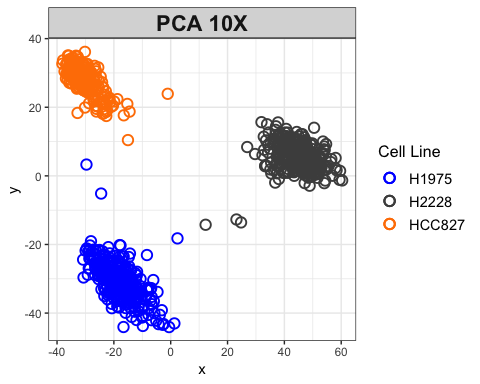
\includegraphics[width=0.5\linewidth]{MINT_Data_Integration_files/figure-latex/1-pca10x-1} 

}

\caption{PCA plot for the 10X dataset. The data tend to group together by cell lines.}\label{fig:1-pca10x}
\end{figure}

PCA plot for 10X data shows that the H2228 cells are most differentiated
from others along the first PC, while the other two are located
similarly along this PC. The 3 clusters are separated along the second
PC. The Drop-seq data have been quality controlled twice and still
exhibit two clusters. One possible explanation is the existence of
doublets (droplets with 2 cells). This highlights the importance of
carefully tuning the experiment parameters.

\begin{Shaded}
\begin{Highlighting}[]
\CommentTok{## CEL-seq2}
\KeywordTok{plotIndiv}\NormalTok{(pca.res.celseq, }\DataTypeTok{legend =} \OtherTok{TRUE}\NormalTok{, }\DataTypeTok{title =} \StringTok{'PCA CEL-seq2'}\NormalTok{, }\DataTypeTok{pch =}\NormalTok{ shape.batch[}\StringTok{'CEL-seq2'}\NormalTok{],}
          \DataTypeTok{col =}\NormalTok{ col.cell, }\DataTypeTok{group =}\NormalTok{ sce4_qc}\OperatorTok{$}\NormalTok{cell_line, }\DataTypeTok{legend.title =} \StringTok{'Cell Line'}\NormalTok{)}
\end{Highlighting}
\end{Shaded}

\begin{figure}[ht]

{\centering 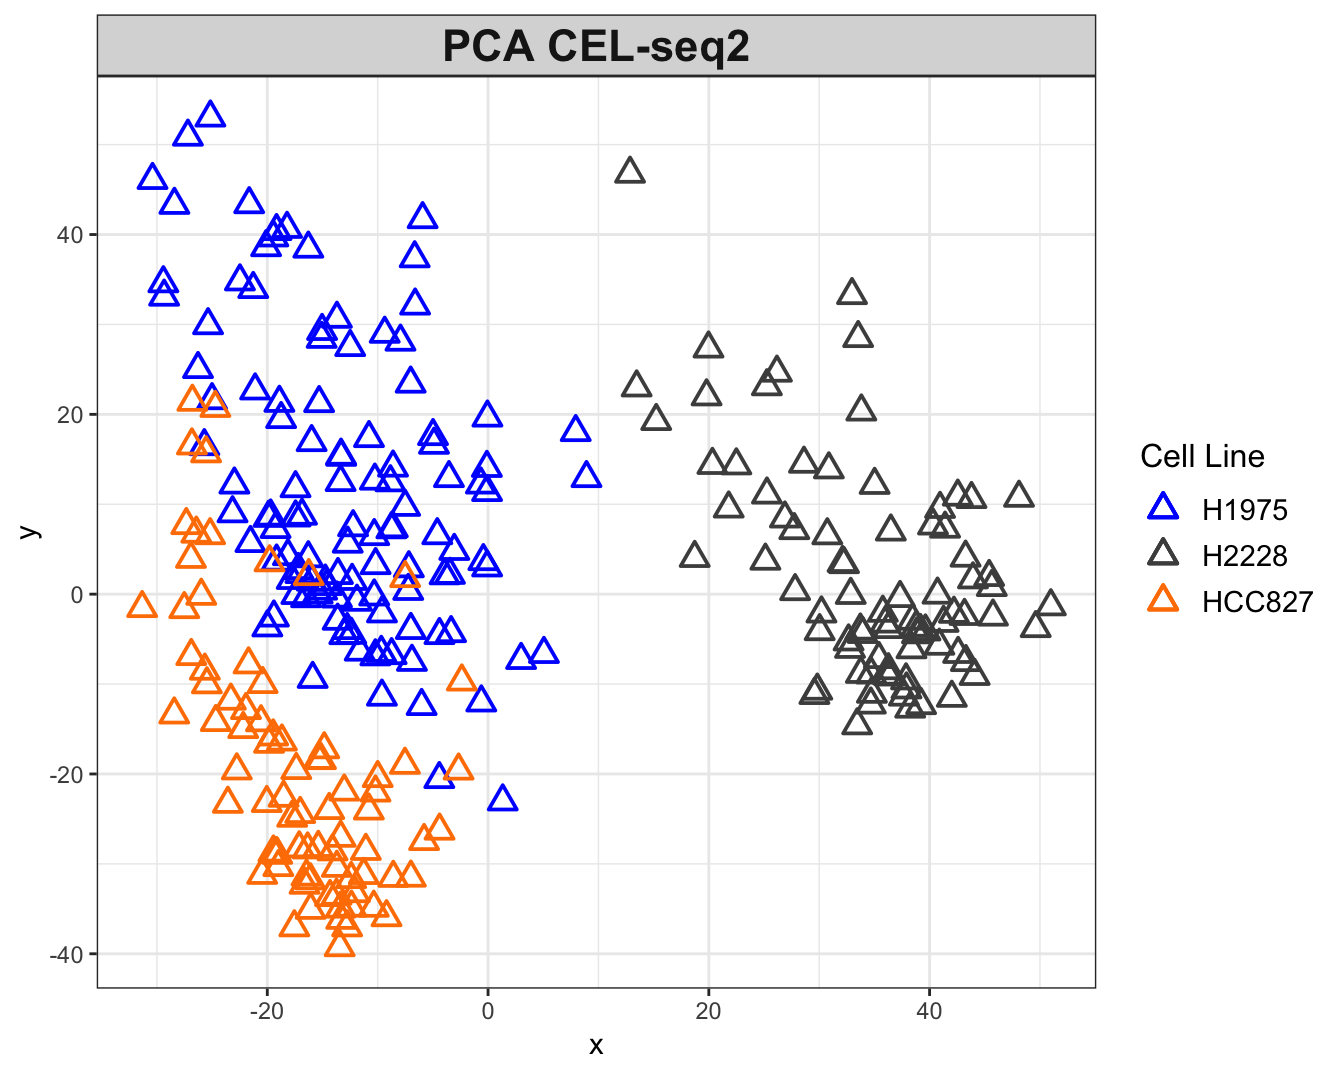
\includegraphics[width=0.5\linewidth]{MINT_Data_Integration_files/figure-latex/1-pcacelseq-1} 

}

\caption{The PCA plots for the CEL-seq2 data. The data are widely scattered in the 2D plane while H2228 cells are relatively distant from the other two.}\label{fig:1-pcacelseq}
\end{figure}

\begin{Shaded}
\begin{Highlighting}[]
\CommentTok{## Drop-seq}
\KeywordTok{plotIndiv}\NormalTok{(pca.res.dropseq, }\DataTypeTok{legend =} \OtherTok{TRUE}\NormalTok{, }\DataTypeTok{title =} \StringTok{'PCA Drop-seq'}\NormalTok{, }\DataTypeTok{pch =}\NormalTok{ shape.batch[}\StringTok{'Drop-seq'}\NormalTok{],}
          \DataTypeTok{col =}\NormalTok{ col.cell, }\DataTypeTok{group =}\NormalTok{ scedrop_qc_qc}\OperatorTok{$}\NormalTok{cell_line, }\DataTypeTok{legend.title =} \StringTok{'Cell Line'}\NormalTok{)}
\end{Highlighting}
\end{Shaded}

\begin{figure}[ht]

{\centering 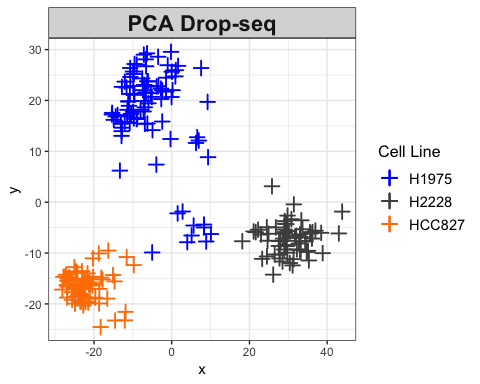
\includegraphics[width=0.5\linewidth]{MINT_Data_Integration_files/figure-latex/1-pcadropseq-1} 

}

\caption{The PCA plots for the Drop-seq data. While H2228 and HCC827 cell data tend to cluster by cell line, the H1975 data exhibit two clusters with negative correlation (on opposite sides of origin). The within-data variation is not consistent between datasets. For instance, the 10X data show a clear grouping structure by cell lines, while this observation is not as strongly supported in other datasets. }\label{fig:1-pcadropseq}
\end{figure}

\hypertarget{pca-on-the-combined-dataset}{%
\section{PCA on the Combined
Dataset}\label{pca-on-the-combined-dataset}}

We now pool/concatenate the datasets for unsupervised analysis. First we
should find out the common genes across the three datasets, as a
requirement for \textbf{P-Integration}:

\begin{Shaded}
\begin{Highlighting}[]
\CommentTok{## find the intersect of the genes for integration}
\NormalTok{list.intersect =}\StringTok{ }\KeywordTok{Reduce}\NormalTok{(intersect, }\KeywordTok{list}\NormalTok{(}
\CommentTok{## the rownames of the original (un-transposed) count matrix will -}
\CommentTok{## output the genes}
  \KeywordTok{rownames}\NormalTok{(}\KeywordTok{logcounts}\NormalTok{(sc10x.norm)),}
  \KeywordTok{rownames}\NormalTok{(}\KeywordTok{logcounts}\NormalTok{(sccel.norm)),}
  \KeywordTok{rownames}\NormalTok{(}\KeywordTok{logcounts}\NormalTok{(scdrop.norm))}
\NormalTok{))}
\end{Highlighting}
\end{Shaded}

Now we can merge the 3 datasets:

\begin{Shaded}
\begin{Highlighting}[]
\CommentTok{## combine the data at their intersection}
\NormalTok{data.combined =}\StringTok{ }\KeywordTok{t}\NormalTok{( }\CommentTok{## transpose of all 3 datasets combined}
  \KeywordTok{data.frame}\NormalTok{(}
    \CommentTok{## the genes from each protocol that match list.intersect}
    \KeywordTok{logcounts}\NormalTok{(sc10x.norm)[list.intersect,],}
    \KeywordTok{logcounts}\NormalTok{(sccel.norm)[list.intersect,],}
    \KeywordTok{logcounts}\NormalTok{(scdrop.norm)[list.intersect,] ))}
\CommentTok{## the number of cells and genes in the intersect dataset}
\KeywordTok{dim}\NormalTok{(data.combined)}
\end{Highlighting}
\end{Shaded}

\begin{verbatim}
## [1]  1401 13575
\end{verbatim}

This matrix includes the count data for the combined dataset. We will
also create 2 vectors of the cell lines and batches for visualisation of
the PCA plots, and also later for the PLS-DA analysis:

\begin{Shaded}
\begin{Highlighting}[]
\CommentTok{## create a factor variable of cell lines}
\CommentTok{## must be in the same order as the data combination}
\NormalTok{cell.line =}\StringTok{ }\KeywordTok{as.factor}\NormalTok{(}\KeywordTok{c}\NormalTok{(sce10x_qc}\OperatorTok{$}\NormalTok{cell_line,}
\NormalTok{                         sce4_qc}\OperatorTok{$}\NormalTok{cell_line,}
\NormalTok{                         scedrop_qc_qc}\OperatorTok{$}\NormalTok{cell_line))}
\CommentTok{## name the factor variable with the cell ID}
\KeywordTok{names}\NormalTok{(cell.line) =}\StringTok{ }\KeywordTok{rownames}\NormalTok{(data.combined)}

\CommentTok{## produce a character vector of batch names}
\CommentTok{## must be in the same order as the data combination}
\NormalTok{batch =}\StringTok{ }\KeywordTok{as.factor}\NormalTok{(}
  \KeywordTok{c}\NormalTok{(}\KeywordTok{rep}\NormalTok{(}\StringTok{'10X'}\NormalTok{,      }\KeywordTok{ncol}\NormalTok{(}\KeywordTok{logcounts}\NormalTok{(sc10x.norm))),}
    \KeywordTok{rep}\NormalTok{(}\StringTok{'CEL-seq2'}\NormalTok{,  }\KeywordTok{ncol}\NormalTok{(}\KeywordTok{logcounts}\NormalTok{(sccel.norm))),}
    \KeywordTok{rep}\NormalTok{(}\StringTok{'Drop-seq'}\NormalTok{, }\KeywordTok{ncol}\NormalTok{(}\KeywordTok{logcounts}\NormalTok{(scdrop.norm))) ))}
\CommentTok{## name it with corresponding cell IDs}
\KeywordTok{names}\NormalTok{(batch) =}\StringTok{ }\KeywordTok{rownames}\NormalTok{(data.combined)}
\end{Highlighting}
\end{Shaded}

We can now perform PCA and visualise the results:

\begin{Shaded}
\begin{Highlighting}[]
\CommentTok{## perform PCA on concatenated data and retrieve 2 PCs}
\NormalTok{pca.combined =}\StringTok{ }\KeywordTok{pca}\NormalTok{(data.combined, }\DataTypeTok{ncomp =} \DecValTok{2}\NormalTok{)}
\end{Highlighting}
\end{Shaded}

\begin{Shaded}
\begin{Highlighting}[]
\CommentTok{## plot the combined pca coloured by batches}
\KeywordTok{plotIndiv}\NormalTok{(pca.combined, }\DataTypeTok{title =} \StringTok{'PCA Combined'}\NormalTok{,}
          \DataTypeTok{pch =}\NormalTok{ batch, }\CommentTok{## shape by cell line}
          \DataTypeTok{group =}\NormalTok{ cell.line, }\CommentTok{## colour by batch}
          \DataTypeTok{legend =} \OtherTok{TRUE}\NormalTok{, }\DataTypeTok{legend.title =} \StringTok{'Study'}\NormalTok{,}
          \DataTypeTok{legend.title.pch =} \StringTok{'Cell Line'}\NormalTok{)}
\end{Highlighting}
\end{Shaded}

\begin{figure}[ht]

{\centering 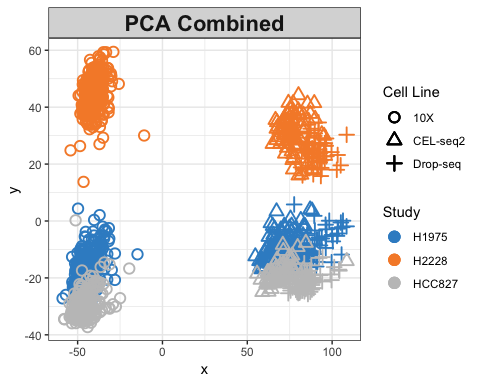
\includegraphics[width=0.6\linewidth]{MINT_Data_Integration_files/figure-latex/1-pcaCombinedByCellline-1} 

}

\caption{The PCA plot for the combined data, coloured by cell lines.}\label{fig:1-pcaCombinedByCellline}
\end{figure}

\begin{Shaded}
\begin{Highlighting}[]
\CommentTok{## plot the combined pca coloured by protocols}
\KeywordTok{plotIndiv}\NormalTok{(pca.combined, }\DataTypeTok{title =} \StringTok{'PCA Combined'}\NormalTok{,}
          \DataTypeTok{pch =}\NormalTok{ cell.line, }\CommentTok{## shape by cell line}
          \DataTypeTok{group =}\NormalTok{ batch, }\CommentTok{## colour by protocol}
          \DataTypeTok{col.per.group =} \KeywordTok{c}\NormalTok{(}\StringTok{'red'}\NormalTok{, }\StringTok{'purple'}\NormalTok{, }\StringTok{'green'}\NormalTok{),}
          \DataTypeTok{legend =} \OtherTok{TRUE}\NormalTok{, }\DataTypeTok{legend.title =} \StringTok{'Study'}\NormalTok{,}
          \DataTypeTok{legend.title.pch =} \StringTok{'Cell Line'}\NormalTok{)}
\end{Highlighting}
\end{Shaded}

\begin{figure}[ht]

{\centering 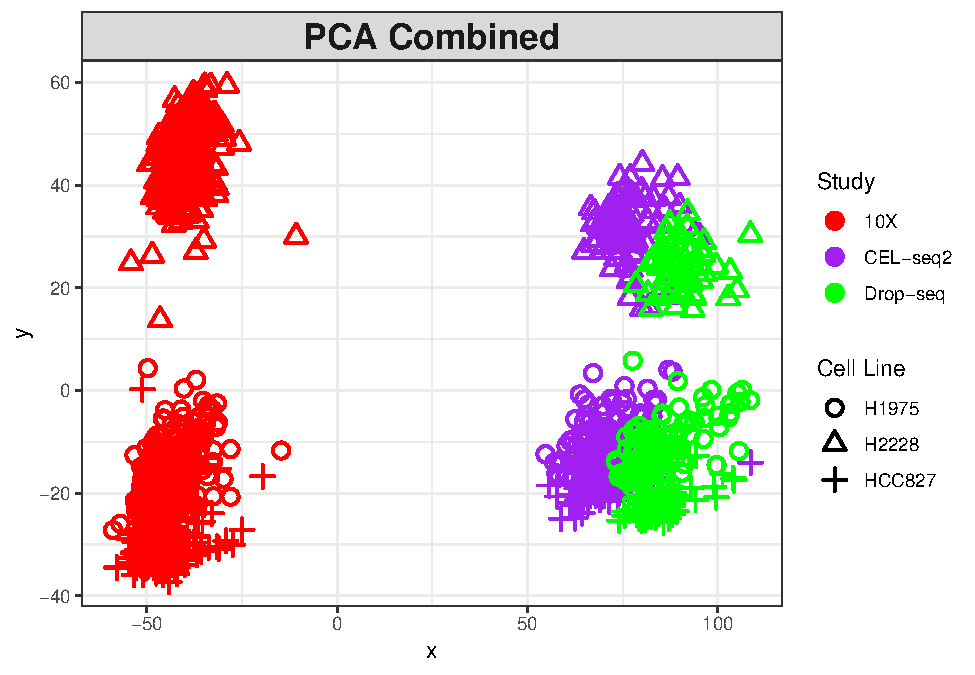
\includegraphics[width=0.6\linewidth]{MINT_Data_Integration_files/figure-latex/1-pcaCombinedByBatch-1} 

}

\caption{The PCA plot for the combined data, coloured by protocols.}\label{fig:1-pcaCombinedByBatch}
\end{figure}

As shown in combined PCA plots above, the protocols are driving the
variation along PC1 (batch effects), while wanted biological variation
is separating the data along PC2. We will next implement the MINT PLS-DA
method on the combined dataset with an aim to account for the batch
effects in discriminating the different cell types.

\hypertarget{mint-to-combine-the-datasets}{%
\section{MINT to Combine the
Datasets}\label{mint-to-combine-the-datasets}}

\emph{MINT} uses \textbf{Projection to Latent Structures - Discriminant
Analysis} to build a learning model on the basis of a training dataset.
Such a predictive model is expected to accurately classify the samples
with unknown cell types in an external learning dataset.

\begin{figure}[ht]

{\centering 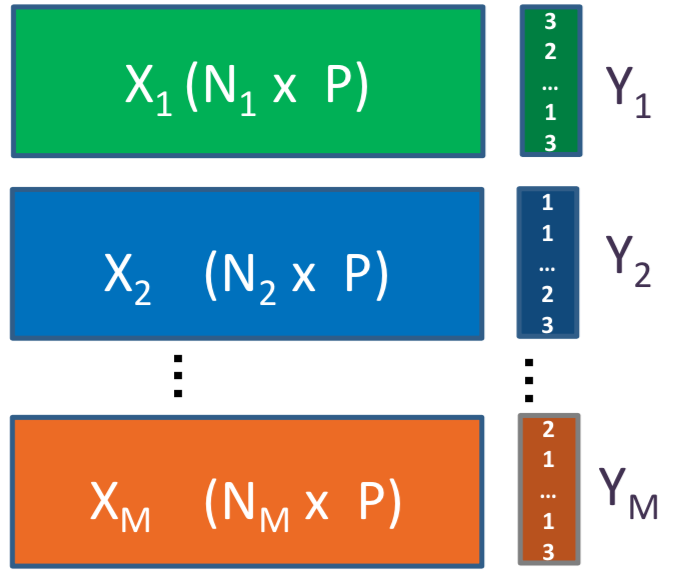
\includegraphics[width=0.3\linewidth]{figures/mintframework} 

}

\caption{P-integration framework using MINT for M independent studies (X) on the same P features. In this setting Y is a vector indicating the class of each cell.}\label{fig:1-graphicsMINT}
\end{figure}

\hypertarget{method}{%
\subsection{Method}\label{method}}

\emph{MINT} finds a set of discriminative latent variables (in this
context, \textbf{linear combinations of gene expression values})
simultaneously in all the datasets, thus leading to PLS-DA Components
(as opposed to PCs in PCA) most influenced by consistent biological
heterogeneity across the studies. Therefore, these components do not
necessarily maximise the variance among the pooled data like what PCs
do, but maximise covariance between the combined data and their classes
(cell lines).

The \emph{mint.plsda} function in \emph{mixOmics} has a set of inputs to
perform the analysis, including:

\begin{itemize}
\tightlist
\item
  \textbf{X}: Which is the original predictor matrix.
\item
  \textbf{Y}: Factor of classes (here, cell lines).
\item
  \textbf{study}: Factor indicating the membership of each sample to
  each of the studies/batches being combined. For a detailed list of
  functions available with \emph{MINT} refer to the documentation.
\end{itemize}

Since PLS-DA is a supervised method, we initially create a vector to
assign each sample to its class/cell.line (Y) and then perform
\emph{MINT}, keeping 2 PLS-DA components:

\begin{Shaded}
\begin{Highlighting}[]
\CommentTok{## create variables needed for MINT}
\CommentTok{## factor variable of cell lines}
\NormalTok{Y =}\StringTok{ }\KeywordTok{as.factor}\NormalTok{(cell.line[}\KeywordTok{rownames}\NormalTok{(data.combined)])}
\CommentTok{## factor variable of studies}
\NormalTok{study =}\StringTok{ }\NormalTok{batch }\CommentTok{## defined in the combined PCA section}
\CommentTok{## MINT on the combined dataset}
\NormalTok{mint.plsda.res =}\StringTok{ }\KeywordTok{mint.plsda}\NormalTok{(}\DataTypeTok{X =}\NormalTok{ data.combined, }\DataTypeTok{Y =}\NormalTok{ Y,}
                             \DataTypeTok{study =}\NormalTok{ study, }\DataTypeTok{ncomp =} \DecValTok{2}\NormalTok{)}
\end{Highlighting}
\end{Shaded}

The outcome is a \emph{mint.plsda} object which can be plotted using
\emph{plotIndiv} function:

\begin{Shaded}
\begin{Highlighting}[]
\CommentTok{## plot the mint.plsda plots for the combined dataset}
\KeywordTok{plotIndiv}\NormalTok{(mint.plsda.res, }\DataTypeTok{group =}\NormalTok{ cell.line,}
          \DataTypeTok{legend  =} \OtherTok{TRUE}\NormalTok{, }\DataTypeTok{subtitle     =} \StringTok{'MINT - Coloured by Cell Line'}\NormalTok{,}
          \DataTypeTok{ellipse =} \OtherTok{FALSE}\NormalTok{, }\DataTypeTok{legend.title =} \StringTok{'Cell Line'}\NormalTok{,}
          \DataTypeTok{legend.title.pch =} \StringTok{'protocol'}\NormalTok{,}
          \DataTypeTok{X.label =} \StringTok{'PLS-DA component 1'}\NormalTok{,}
          \DataTypeTok{Y.label =} \StringTok{'PLS-DA component 2'}\NormalTok{)}
\end{Highlighting}
\end{Shaded}

\begin{figure}[ht]

{\centering 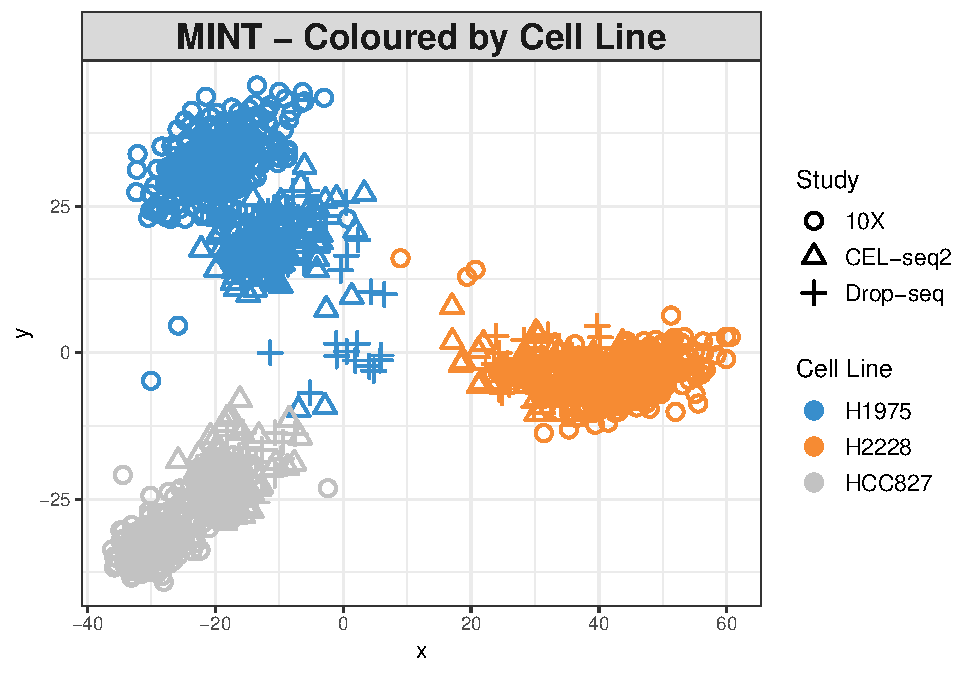
\includegraphics[width=0.5\linewidth]{MINT_Data_Integration_files/figure-latex/1-MINTplots1-1} 

}

\caption{The MINT PLS-DA plot for the combined dataset. Data points are coloured by cell lines.}\label{fig:1-MINTplots1}
\end{figure}

As seen in the PLS-DA plots, the data are differentiated mainly by their
cell lines. The effects of batches are not fully eliminated yet.

\hypertarget{optimum-number-of-components}{%
\subsection{Optimum Number of
Components}\label{optimum-number-of-components}}

So far, we presented a \emph{MINT} PLS-DA with only 2 components. We can
look at the calassification error rates over different choices of number
of components using \emph{perf} function in \emph{mixOmics}, which
evaluates the performance of the fitted PLS models internally using
Leave-One-Group-Out Cross Validation (LOGOCV) in \emph{MINT} (M-Fold
Cross-Validation is also available). Refer to the documentation for more
details about \emph{perf} arguments.

\begin{Shaded}
\begin{Highlighting}[]
\CommentTok{## retrieve 5 PLS-DA components using MINT}
\NormalTok{mint.plsda.res =}\StringTok{ }\KeywordTok{mint.plsda}\NormalTok{(}\DataTypeTok{X =}\NormalTok{ data.combined, }\DataTypeTok{Y =}\NormalTok{ Y,}
                                 \DataTypeTok{study =}\NormalTok{ study, }\DataTypeTok{ncomp =} \DecValTok{5}\NormalTok{)}
\CommentTok{## perform cross validation and calculate classification error rates}
\KeywordTok{set.seed}\NormalTok{(}\DecValTok{12321}\NormalTok{)  }\CommentTok{# for reproducibility of the results}
\NormalTok{perf.mint.plsda.res =}\StringTok{ }\KeywordTok{perf}\NormalTok{(mint.plsda.res,}
          \DataTypeTok{progressBar =} \OtherTok{FALSE}\NormalTok{)}
\end{Highlighting}
\end{Shaded}

We now plot the output:

\begin{Shaded}
\begin{Highlighting}[]
\CommentTok{## plot the classification error rate vs number of components}
\KeywordTok{plot}\NormalTok{(perf.mint.plsda.res, }\DataTypeTok{col =} \KeywordTok{color.mixo}\NormalTok{(}\DecValTok{5}\OperatorTok{:}\DecValTok{7}\NormalTok{))}
\end{Highlighting}
\end{Shaded}

\begin{figure}[ht]

{\centering 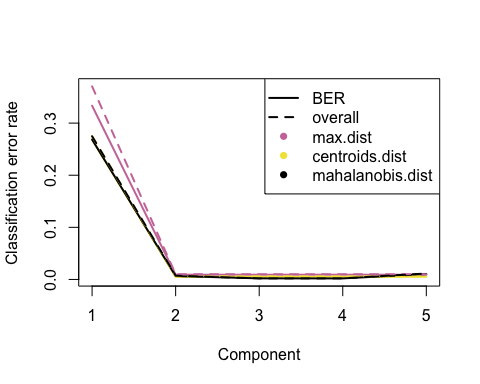
\includegraphics[width=0.5\linewidth]{MINT_Data_Integration_files/figure-latex/1-perfPlot-1} 

}

\caption{The classification error rate for different number of PLS-DA components showing Balanced and Overall Error Rates, each comprising three distance measures. The distances measure how far any given data point is from the mean of its class.}\label{fig:1-perfPlot}
\end{figure}

As seen in the plot above, at ncomp = 2 the model has the optimum
performance for all distances in terms of Balanced and Overall Error
Rate, as there is not a considerable drop in error rates for further
components (see supplemental information from \citep{R-mixOmics} for
more details about the prediction distances). Additional numerical
outputs are available to stratify the error rates per cell
line/protocol/distance measure:

\begin{Shaded}
\begin{Highlighting}[]
\NormalTok{perf.mint.plsda.res}\OperatorTok{$}\NormalTok{global.error}\OperatorTok{$}\NormalTok{BER }\CommentTok{## further error diagnostics }
\end{Highlighting}
\end{Shaded}

\begin{verbatim}
##           max.dist centroids.dist mahalanobis.dist
## comp 1 0.333333333    0.268431385      0.268431385
## comp 2 0.009072456    0.005218891      0.006503413
## comp 3 0.009072456    0.005218891      0.002088392
## comp 4 0.009072456    0.005218891      0.002007587
## comp 5 0.009072456    0.005218891      0.010356977
\end{verbatim}

Also, the function outputs the optimal number of components via the
\emph{choice.ncomp} attribute.

\begin{Shaded}
\begin{Highlighting}[]
\CommentTok{## number of variables to select in each component}
\NormalTok{perf.mint.plsda.res}\OperatorTok{$}\NormalTok{choice.ncomp}
\end{Highlighting}
\end{Shaded}

\begin{verbatim}
##         max.dist centroids.dist mahalanobis.dist
## overall        2              2                2
## BER            2              2                2
\end{verbatim}

\hypertarget{sparse-mint-pls-da}{%
\subsection{Sparse MINT PLS-DA}\label{sparse-mint-pls-da}}

At this section, we investigate the performance of \emph{MINT} with
variable selection (we call it sparse MINT PLSDA or MINT sPLS-DA). This
helps by eliminating the noisy variables (here genes) from the model to
better interpret the signal coming from the primary variables. At this
stage, we will ask the model to keep 50 variables with highest loadings
on each component. The number of variables to keep should be set as a
vector into \emph{keepX} argument in \emph{mint.splsda} (refer to the
documentation for more details):

\begin{Shaded}
\begin{Highlighting}[]
\CommentTok{## number of variables to keep in each component}
\NormalTok{list.keepX =}\StringTok{ }\KeywordTok{c}\NormalTok{(}\DecValTok{50}\NormalTok{,}\DecValTok{50}\NormalTok{) }
\CommentTok{## perform sparse PLS-DA using MINT with 2 components}
\NormalTok{mint.splsda.res =}\StringTok{ }\KeywordTok{mint.splsda}\NormalTok{(}\DataTypeTok{X =}\NormalTok{ data.combined, }\DataTypeTok{Y =}\NormalTok{ Y,}
                              \DataTypeTok{study =}\NormalTok{ study, }\DataTypeTok{ncomp =} \DecValTok{2}\NormalTok{, }\DataTypeTok{keepX =}\NormalTok{ list.keepX)}
\end{Highlighting}
\end{Shaded}

Plot the sparse \emph{MINT} object:

\begin{Shaded}
\begin{Highlighting}[]
\KeywordTok{plotIndiv}\NormalTok{(mint.splsda.res,}
          \DataTypeTok{legend  =} \OtherTok{TRUE}\NormalTok{, }\DataTypeTok{subtitle =} \StringTok{'Sparse MINT'}\NormalTok{, }\DataTypeTok{ellipse =} \OtherTok{TRUE}\NormalTok{,}
          \DataTypeTok{X.label =} \StringTok{'sPLS-DA component 1'}\NormalTok{, }
          \DataTypeTok{Y.label =} \StringTok{'sPLS-DA component 2'}\NormalTok{,}
          \DataTypeTok{group =}\NormalTok{ Y, }\CommentTok{## colour by cell line}
          \DataTypeTok{legend.title =} \StringTok{'Cell Line'}\NormalTok{,}
          \DataTypeTok{legend.title.pch =} \StringTok{'Protocol'}\NormalTok{)}
\end{Highlighting}
\end{Shaded}

\begin{figure}[ht]

{\centering 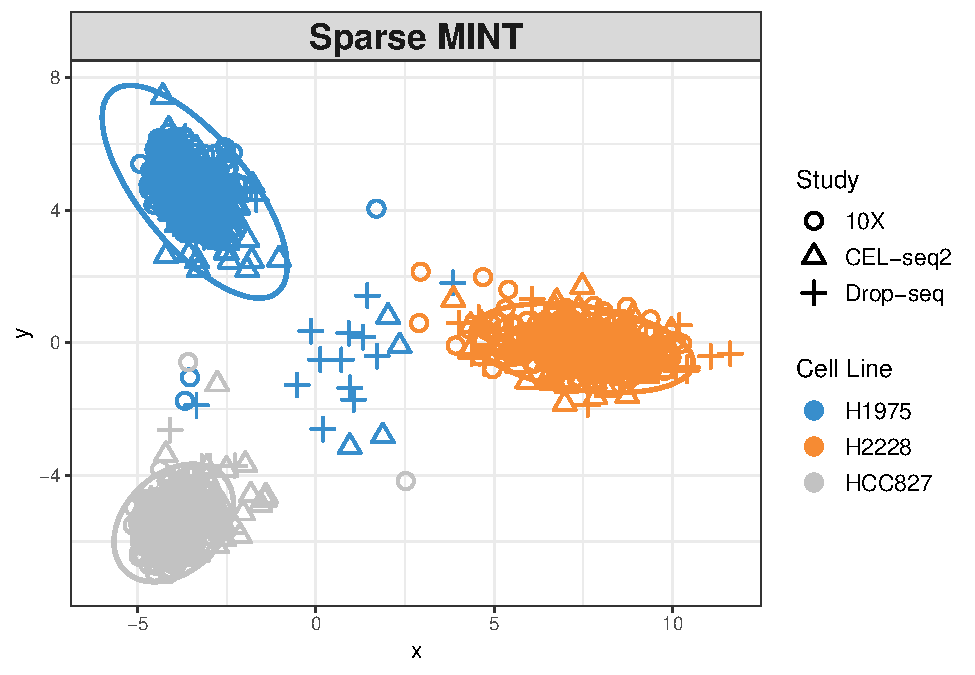
\includegraphics[width=0.5\linewidth]{MINT_Data_Integration_files/figure-latex/1-sMINTplots1-1} 

}

\caption{The Sparse MINT PLS-DA plot for the combined dataset. Data points are coloured by cell lines.}\label{fig:1-sMINTplots1}
\end{figure}

The clusters are now more refined compared to the non-sparse method. The
effects of batches are now almost removed, and the samples from the 10X
dataset seem equally differentiated as the others.

\hypertarget{choice-of-parameters}{%
\subsection{Choice of Parameters}\label{choice-of-parameters}}

Previously, we chose 50 variables for a sparse analysis. The optimal
number of the variables can be determined for each component using the
\emph{tune} function. The \emph{test.keepX} argument specifies a vector
of the candidate numbers of variables in each PLS-DA component to be
evaluated. We will try 5,10,\ldots{},35,40,\ldots{},70 and 100
variables, and also record the runtime. We will separately tune each
component for better visualisation but tuning can be done in one step
for all components.

\begin{Shaded}
\begin{Highlighting}[]
\CommentTok{## tune MINT for component 1 and then 2 and record the run time}
\CommentTok{## we tune individual components for visualisation purposes}
\CommentTok{## one can run only the tune.mint.c2 without already.tested.X}
\NormalTok{start.time =}\StringTok{ }\KeywordTok{Sys.time}\NormalTok{()}
\CommentTok{## tune using a test set of variable numbers}
\CommentTok{## component 1}
\NormalTok{tune.mint.c1 =}\StringTok{ }\KeywordTok{tune}\NormalTok{(}
  \DataTypeTok{X =}\NormalTok{ data.combined, }\DataTypeTok{Y =}\NormalTok{ Y, }\DataTypeTok{study =}\NormalTok{ study, }\DataTypeTok{ncomp =} \DecValTok{1}\NormalTok{,}
  \CommentTok{## assess numbers 5,10,15...50,60,70,...100:}
  \DataTypeTok{test.keepX =} \KeywordTok{c}\NormalTok{(}\KeywordTok{seq}\NormalTok{(}\DecValTok{5}\NormalTok{,}\DecValTok{35}\NormalTok{,}\DecValTok{5}\NormalTok{),}\KeywordTok{seq}\NormalTok{(}\DecValTok{40}\NormalTok{,}\DecValTok{70}\NormalTok{,}\DecValTok{10}\NormalTok{), }\DecValTok{100}\NormalTok{), }\DataTypeTok{method =} \StringTok{'mint.splsda'}\NormalTok{,}
  \CommentTok{## use all distances to estimate the classification error rate}
  \DataTypeTok{dist =} \KeywordTok{c}\NormalTok{(}\StringTok{'max.dist'}\NormalTok{,  }\StringTok{'centroids.dist'}\NormalTok{, }\StringTok{'mahalanobis.dist'}\NormalTok{),}
  \DataTypeTok{progressBar =} \OtherTok{FALSE}
\NormalTok{)}
\CommentTok{## component 1 to 2}
\NormalTok{tune.mint.c2 =}\StringTok{ }\KeywordTok{tune}\NormalTok{(}
  \DataTypeTok{X =}\NormalTok{ data.combined, }\DataTypeTok{Y =}\NormalTok{ Y, }\DataTypeTok{study =}\NormalTok{ study, }\DataTypeTok{ncomp =} \DecValTok{2}\NormalTok{,}
  \CommentTok{## already tuned component 1}
  \DataTypeTok{already.tested.X =}\NormalTok{ tune.mint.c1}\OperatorTok{$}\NormalTok{choice.keepX,}
  \DataTypeTok{test.keepX =} \KeywordTok{c}\NormalTok{(}\KeywordTok{seq}\NormalTok{(}\DecValTok{5}\NormalTok{,}\DecValTok{35}\NormalTok{,}\DecValTok{5}\NormalTok{),}\KeywordTok{seq}\NormalTok{(}\DecValTok{40}\NormalTok{,}\DecValTok{70}\NormalTok{,}\DecValTok{10}\NormalTok{), }\DecValTok{100}\NormalTok{), }\DataTypeTok{method =} \StringTok{'mint.splsda'}\NormalTok{,}
  \DataTypeTok{dist =} \KeywordTok{c}\NormalTok{(}\StringTok{'max.dist'}\NormalTok{,  }\StringTok{'centroids.dist'}\NormalTok{, }\StringTok{'mahalanobis.dist'}\NormalTok{),}
  \DataTypeTok{progressBar =} \OtherTok{FALSE}
\NormalTok{)}
\NormalTok{end.time =}\StringTok{ }\KeywordTok{Sys.time}\NormalTok{()}
\CommentTok{## see how long it takes to find the optimum number of variables:}
\NormalTok{run.time =}\StringTok{  }\NormalTok{end.time }\OperatorTok{-}\StringTok{ }\NormalTok{start.time}
\end{Highlighting}
\end{Shaded}

It took less than 5 minutes to evaluate the chosen test set of variables
using a 2.6 GHz Dual-core Intel Core i5 processor (8GB RAM). It is
always more practical to look into a coarse grid at first and then
refine it when the right neighbourhood is found. We now look at the
optimum number of components chosen and their corresponding Balanced
Error Rate:

\begin{Shaded}
\begin{Highlighting}[]
\CommentTok{## look at the optimal selected variables for each PC}
\NormalTok{tune.mint.c2}\OperatorTok{$}\NormalTok{choice.keepX}
\end{Highlighting}
\end{Shaded}

\begin{verbatim}
## comp 1 comp 2 
##     35     10
\end{verbatim}

\begin{Shaded}
\begin{Highlighting}[]
\CommentTok{## plot the error rates for all test variable numbers}
\KeywordTok{par}\NormalTok{(}\DataTypeTok{mfrow=}\KeywordTok{c}\NormalTok{(}\DecValTok{1}\NormalTok{,}\DecValTok{3}\NormalTok{))}
\KeywordTok{plot}\NormalTok{(tune.mint.c1, }\DataTypeTok{col =} \StringTok{'darkred'}\NormalTok{)}
\KeywordTok{plot}\NormalTok{(tune.mint.c2, }\DataTypeTok{col =} \StringTok{'darkblue'}\NormalTok{)}
\end{Highlighting}
\end{Shaded}

\begin{figure}[ht]

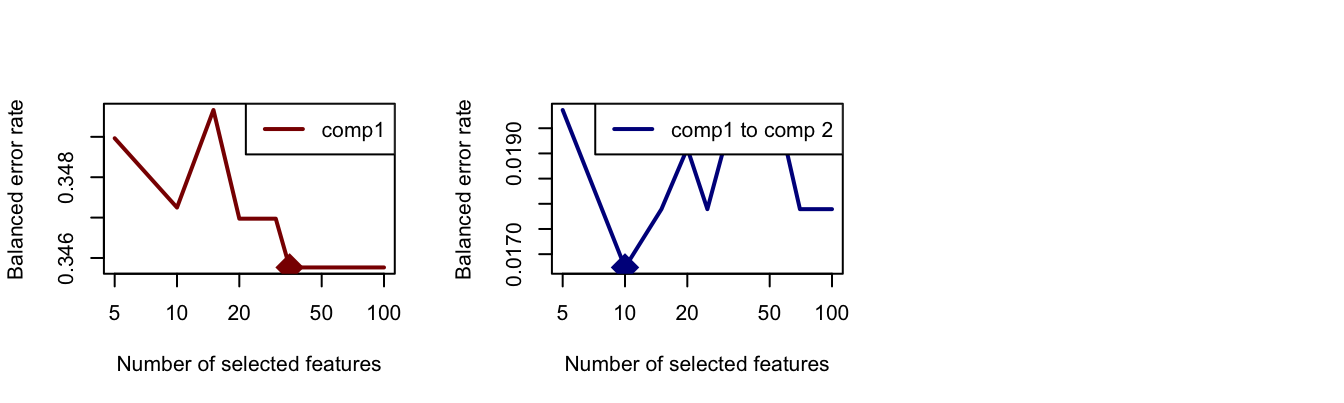
\includegraphics[width=1\linewidth]{MINT_Data_Integration_files/figure-latex/1-BERplot-1} \hfill{}

\caption{The Balanced Error Rate as a function of number of variables in PLS-DA components 1 (left) and 2 (right). }\label{fig:1-BERplot}
\end{figure}

The optimum numbers of variables for each component are shown using a
diamond mark in plots above, which are 35 for the first and 10 for the
second one.

We now re-run the sparse \emph{MINT} using optimum parameters:

\begin{Shaded}
\begin{Highlighting}[]
\CommentTok{## run sparse mint using optimum parameters:}
\NormalTok{mint.splsda.tuned.res =}\StringTok{ }\KeywordTok{mint.splsda}\NormalTok{( }\DataTypeTok{X =}\NormalTok{data.combined, }\DataTypeTok{Y =}\NormalTok{ Y,}
                              \DataTypeTok{study =}\NormalTok{ study, }\DataTypeTok{ncomp =} \DecValTok{2}\NormalTok{,  }
                              \DataTypeTok{keepX =}\NormalTok{ tune.mint.c2}\OperatorTok{$}\NormalTok{choice.keepX)}
\end{Highlighting}
\end{Shaded}

Next, we plot the \emph{mint.splsda} object with global variables (for
the combined dataset):

\begin{Shaded}
\begin{Highlighting}[]
\CommentTok{## plot the tuned mint.splsda plot for the combined dataset}
\KeywordTok{plotIndiv}\NormalTok{(mint.splsda.tuned.res, }\DataTypeTok{study =} \StringTok{'global'}\NormalTok{, }\DataTypeTok{legend =} \OtherTok{TRUE}\NormalTok{,}
          \DataTypeTok{title =} \StringTok{'MINT sPLS-DA'}\NormalTok{,  }\DataTypeTok{subtitle =} \StringTok{'Global'}\NormalTok{, }\DataTypeTok{ellipse=}\OtherTok{TRUE}\NormalTok{)}
\end{Highlighting}
\end{Shaded}

\begin{figure}[ht]

{\centering 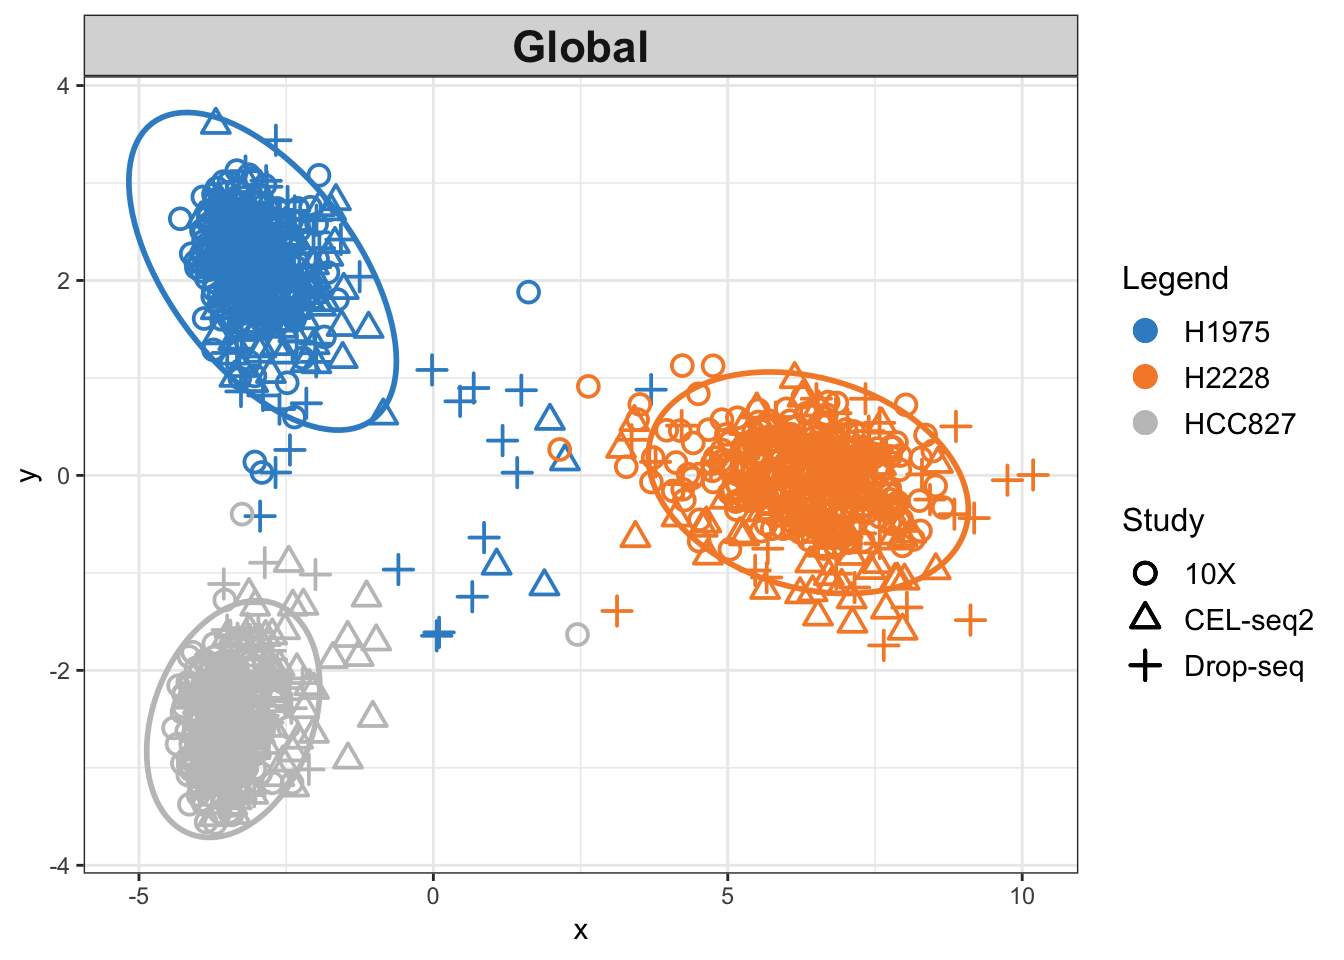
\includegraphics[width=0.5\linewidth]{MINT_Data_Integration_files/figure-latex/1-sMINTtunedPlot-1} 

}

\caption{The tuned MINT sPLS-DA plot for the combined data. While there are still a number of samples that are not well classified, the clusters are more refined when we perform variable selection.}\label{fig:1-sMINTtunedPlot}
\end{figure}

We can also look at the dataset per protocol using \emph{all.partial} as
the input for the \emph{study} argument:

\begin{Shaded}
\begin{Highlighting}[]
\CommentTok{## tuned mint.splsda plot for each protocol}
\KeywordTok{plotIndiv}\NormalTok{(mint.splsda.tuned.res, }\DataTypeTok{study =} \StringTok{'all.partial'}\NormalTok{,  }\DataTypeTok{title =} \StringTok{'MINT sPLS-DA'}\NormalTok{, }
          \DataTypeTok{subtitle =} \KeywordTok{c}\NormalTok{(}\StringTok{'10X'}\NormalTok{, }\StringTok{'CEL-seq2'}\NormalTok{, }\StringTok{'Drop-seq'}\NormalTok{))}
\end{Highlighting}
\end{Shaded}

\begin{figure}[ht]

{\centering 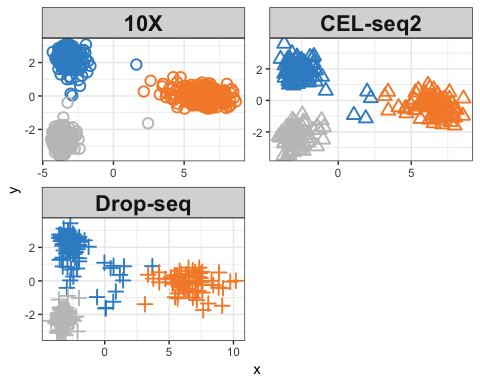
\includegraphics[width=0.95\linewidth]{MINT_Data_Integration_files/figure-latex/1-sMINTtunedPartial-1} 

}

\caption{MINT sPLS-DA components for each individual protocol coloured by cell line.}\label{fig:1-sMINTtunedPartial}
\end{figure}

The majority of samples from the 10X data are well classified, while the
method struggles to classify some samples from H1975 samples in the
Drop-seq and CEL-seq2 datasets.

\hypertarget{performance-assessment}{%
\subsection{Performance Assessment}\label{performance-assessment}}

We now can evaluate the classification performance of the final model
using \emph{perf} function. We will use the maximum distance measure.

\begin{Shaded}
\begin{Highlighting}[]
\KeywordTok{set.seed}\NormalTok{(}\DecValTok{12321}\NormalTok{)  }\CommentTok{# for reproducibility of the results}
\CommentTok{## perform classification with leave-one-group-out cross validation }
\NormalTok{perf.mint.final =}\StringTok{ }\KeywordTok{perf}\NormalTok{(mint.splsda.res, }\DataTypeTok{progressBar =} \OtherTok{FALSE}\NormalTok{, }\DataTypeTok{dist =} \StringTok{'max.dist'}\NormalTok{)}
\CommentTok{## classification error rate}
\NormalTok{perf.mint.final}\OperatorTok{$}\NormalTok{global.error}
\end{Highlighting}
\end{Shaded}

\begin{verbatim}
## $BER
##          max.dist
## comp 1 0.35106644
## comp 2 0.01156069
## 
## $overall
##          max.dist
## comp 1 0.33333333
## comp 2 0.01284797
## 
## $error.rate.class
## $error.rate.class$max.dist
##           comp 1     comp 2
## H1975  0.2408478 0.03468208
## H2228  0.0000000 0.00000000
## HCC827 0.8123515 0.00000000
\end{verbatim}

The balanced and overall error rates are 1.2 and 1.3 percent
respectively, while the model classifies the H2228 cell types with zero
error rate.

\hypertarget{roc-curves}{%
\subsection{ROC Curves}\label{roc-curves}}

Another available visualisation tool is the ROC (Receiver Operating
Characteristic) curves for each study (or all) to evaluate the
prediction accuracy of a classification mode. In a ROC curve the true
positive rate (Sensitivity) is plotted against the false positive rate
(100-Specificity) for different classification thresholds. This method
should be interpreted carefully in such multivariate analysis where no
clear cut-off threshold can be considered.

\begin{Shaded}
\begin{Highlighting}[]
\CommentTok{## ROC curves for both components}
\NormalTok{auc.mint.splsda1 =}\StringTok{ }\KeywordTok{auroc}\NormalTok{(mint.splsda.tuned.res, }\DataTypeTok{roc.comp =} \DecValTok{1}\NormalTok{, }\DataTypeTok{roc.study=}\StringTok{'CEL-seq2'}\NormalTok{)}
\end{Highlighting}
\end{Shaded}

\begin{center}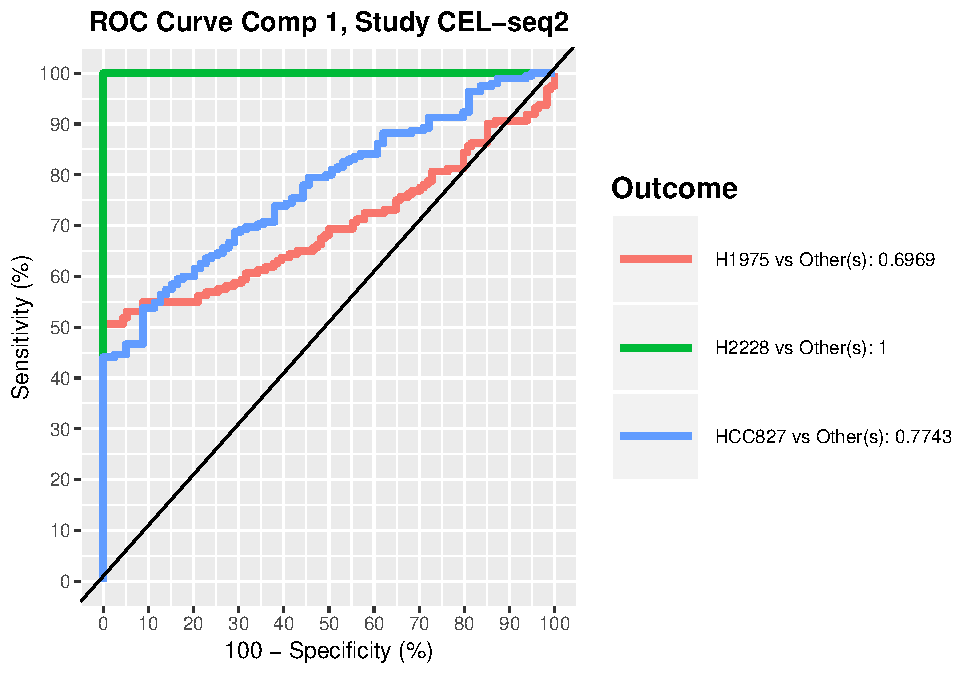
\includegraphics[width=0.5\linewidth]{MINT_Data_Integration_files/figure-latex/1-roc-1} \end{center}

\begin{Shaded}
\begin{Highlighting}[]
\NormalTok{auc.mint.splsda2 =}\StringTok{ }\KeywordTok{auroc}\NormalTok{(mint.splsda.tuned.res, }\DataTypeTok{roc.comp =} \DecValTok{2}\NormalTok{, }\DataTypeTok{roc.study=}\StringTok{'CEL-seq2'}\NormalTok{)}
\end{Highlighting}
\end{Shaded}

\begin{center}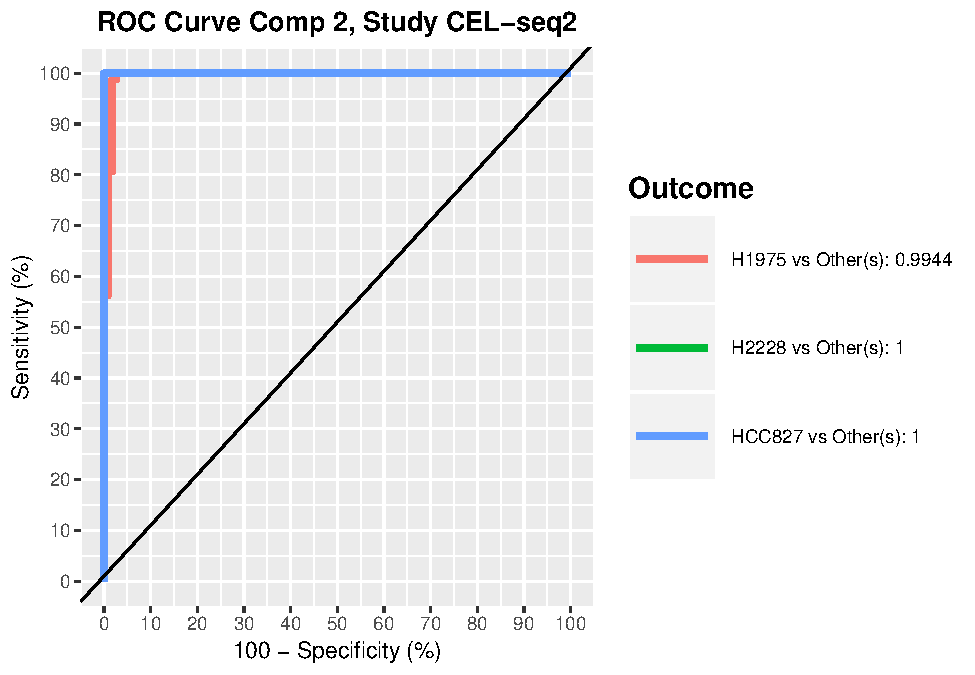
\includegraphics[width=0.5\linewidth]{MINT_Data_Integration_files/figure-latex/1-roc-2} \end{center}

For a perfect model the curve would go through the upper left corner,
while the black line represents a perfectly random classification model.

ROC plots show that for CEL-seq data, the model has relatively low
prediction accuracy for HCC827 and H1975 samples in the first component,
while it has high prediction accuracy for all samples in the second
component. This was also apparent in sPLS-DA plot, as HCC827 and H1975
samples were not separated along the first PLSDA component for CEL-seq
data, while most of samples were differentiated along the second
component by their cell lines.

\hypertarget{session-information}{%
\section{Session Information}\label{session-information}}

\begin{Shaded}
\begin{Highlighting}[]
\CommentTok{## session information to build this vignette}
\KeywordTok{sessionInfo}\NormalTok{()}
\end{Highlighting}
\end{Shaded}

\begin{verbatim}
## R version 3.5.0 (2018-04-23)
## Platform: x86_64-apple-darwin15.6.0 (64-bit)
## Running under: macOS  10.14
## 
## Matrix products: default
## BLAS: /Library/Frameworks/R.framework/Versions/3.5/Resources/lib/libRblas.0.dylib
## LAPACK: /Library/Frameworks/R.framework/Versions/3.5/Resources/lib/libRlapack.dylib
## 
## locale:
## [1] en_AU.UTF-8/en_AU.UTF-8/en_AU.UTF-8/C/en_AU.UTF-8/en_AU.UTF-8
## 
## attached base packages:
##  [1] grid      parallel  stats4    stats     graphics  grDevices utils    
##  [8] datasets  methods   base     
## 
## other attached packages:
##  [1] tibble_1.4.2                VennDiagram_1.6.20         
##  [3] futile.logger_1.4.3         scater_1.9.24              
##  [5] scran_1.9.39                mixOmics_6.4.6             
##  [7] ggplot2_3.1.0               lattice_0.20-38            
##  [9] MASS_7.3-51.1               SingleCellExperiment_1.3.12
## [11] SummarizedExperiment_1.11.6 DelayedArray_0.7.49        
## [13] BiocParallel_1.15.15        matrixStats_0.54.0         
## [15] Biobase_2.41.2              GenomicRanges_1.33.14      
## [17] GenomeInfoDb_1.17.4         IRanges_2.15.19            
## [19] S4Vectors_0.19.24           BiocGenerics_0.27.1        
## [21] knitr_1.20                 
## 
## loaded via a namespace (and not attached):
##  [1] viridis_0.5.1             dynamicTreeCut_1.63-1    
##  [3] edgeR_3.23.7              tidyr_0.8.2              
##  [5] viridisLite_0.3.0         DelayedMatrixStats_1.3.11
##  [7] ellipse_0.4.1             assertthat_0.2.0         
##  [9] statmod_1.4.30            highr_0.7                
## [11] vipor_0.4.5               GenomeInfoDbData_1.2.0   
## [13] yaml_2.2.0                pillar_1.3.0             
## [15] backports_1.1.2           glue_1.3.0               
## [17] limma_3.37.10             digest_0.6.18            
## [19] RColorBrewer_1.1-2        XVector_0.21.4           
## [21] colorspace_1.3-2          htmltools_0.3.6          
## [23] Matrix_1.2-15             plyr_1.8.4               
## [25] pkgconfig_2.0.2           bookdown_0.7             
## [27] zlibbioc_1.27.0           purrr_0.2.5              
## [29] corpcor_1.6.9             scales_1.0.0             
## [31] HDF5Array_1.9.19          RSpectra_0.13-1          
## [33] withr_2.1.2               lazyeval_0.2.1           
## [35] magrittr_1.5              crayon_1.3.4             
## [37] evaluate_0.12             beeswarm_0.2.3           
## [39] tools_3.5.0               formatR_1.5              
## [41] stringr_1.3.1             Rhdf5lib_1.3.3           
## [43] munsell_0.5.0             locfit_1.5-9.1           
## [45] lambda.r_1.2.3            bindrcpp_0.2.2           
## [47] compiler_3.5.0            rlang_0.3.0.1            
## [49] rhdf5_2.25.11             RCurl_1.95-4.11          
## [51] BiocNeighbors_0.99.22     rstudioapi_0.8           
## [53] igraph_1.2.2              labeling_0.3             
## [55] bitops_1.0-6              rmarkdown_1.10           
## [57] gtable_0.2.0              codetools_0.2-15         
## [59] rARPACK_0.11-0            reshape2_1.4.3           
## [61] R6_2.3.0                  gridExtra_2.3            
## [63] dplyr_0.7.8               bindr_0.1.1              
## [65] rprojroot_1.3-2           futile.options_1.0.1     
## [67] ggbeeswarm_0.6.0          stringi_1.2.4            
## [69] Rcpp_1.0.0                tidyselect_0.2.5         
## [71] xfun_0.4
\end{verbatim}

\hypertarget{troubleshoots}{%
\section{Troubleshoots}\label{troubleshoots}}

\hypertarget{bioconductor}{%
\subsection{Bioconductor}\label{bioconductor}}

You can check out
\href{https://bioconductor.org/install/\#troubleshoot-bioconductor-packages}{Bioconductor's
troubleshoot page}

\hypertarget{mixomics}{%
\subsection{mixOmics}\label{mixomics}}

In case you are having issues with \emph{mixOmics}, please look it up at
the \href{https://bitbucket.org/klecao/package-mixomics/issues}{mixOmics
issues page} and if you did not find your solution, create a new issue.
You can also check out or submit your questions on
\href{https://stackoverflow.com/search?q=mixomics}{stackoverflow
forums}.

\hypertarget{mac-os}{%
\subsection{mac OS}\label{mac-os}}

\begin{itemize}
\item
  \textbf{Compilation error while installing libraries from
  binconductor} This could be due to the fortran compiler not being
  updated for newer R versions. You can go to
  \href{https://thecoatlessprofessor.com/programming/rcpp-rcpparmadillo-and-os-x-mavericks--lgfortran-and--lquadmath-error/}{this
  website} and get the instructions on how to install the latest
  gfortran for your R and mac OS version.
\item
  \textbf{Unable to import \emph{rgl} library } Ensure you have the
  \href{https://www.xquartz.org/}{latest version of XQuartz} installed.
\end{itemize}

\hypertarget{identifying-gene-signature-using-mint}{%
\chapter{Identifying Gene Signature using
MINT}\label{identifying-gene-signature-using-mint}}

\hypertarget{identifying-molecular-signatures-using-mint-splsda}{%
\section{Identifying Molecular Signatures using MINT
sPLSDA}\label{identifying-molecular-signatures-using-mint-splsda}}

This section follows up on the Data Integration vignette. The aim here
is to find the gene signature characterising the cell lines using the
MINT sPLS-DA model and also to make relevant comparisons.

The following topics are covered in details in the previous vignette and
thus will not be expanded:

\begin{itemize}
\tightlist
\item
  The instructions on installation of the required packages
\item
  Data normalisation method using \emph{scran} package
\end{itemize}

\hypertarget{r-scripts-1}{%
\section{R Scripts}\label{r-scripts-1}}

The R scripts are available at
\href{https://github.com/AJABADI/MINT_sPLSDA/blob/master/02-Signature.R}{this
link}.

\hypertarget{libraries-1}{%
\section{Libraries}\label{libraries-1}}

\begin{Shaded}
\begin{Highlighting}[]
\CommentTok{## load the required libraries}
\KeywordTok{library}\NormalTok{(SingleCellExperiment)}
\KeywordTok{library}\NormalTok{(mixOmics)}
\KeywordTok{library}\NormalTok{(scran)}
\KeywordTok{library}\NormalTok{(scater)}
\KeywordTok{library}\NormalTok{(knitr)}
\KeywordTok{library}\NormalTok{(VennDiagram)}
\KeywordTok{library}\NormalTok{(tibble)}
\end{Highlighting}
\end{Shaded}

\hypertarget{data-1}{%
\section{Data}\label{data-1}}

The data need to be loaded only if the vignette files are being run
separately (and not as a book). The raw and normalised data are loaded
from the Data Integration vignette. You can load them directly from
github:

\begin{Shaded}
\begin{Highlighting}[]
\CommentTok{## load from github}
\CommentTok{## raw}
\NormalTok{RawURL=}\StringTok{'https://tinyurl.com/sincell-with-class-RData-LuyiT'}
\KeywordTok{load}\NormalTok{(}\KeywordTok{url}\NormalTok{(RawURL))}
\end{Highlighting}
\end{Shaded}

Alternatively, you can download and load directly into R environment:

\begin{Shaded}
\begin{Highlighting}[]
\CommentTok{## or load from local directory, change to your own}
\KeywordTok{load}\NormalTok{(io}\OperatorTok{$}\NormalTok{local.sincell)}
\end{Highlighting}
\end{Shaded}

\begin{Shaded}
\begin{Highlighting}[]
\CommentTok{## normalise the QC'ed count matrices}
\NormalTok{sc10x.norm =}\StringTok{  }\KeywordTok{computeSumFactors}\NormalTok{(sce10x_qc) }\CommentTok{## deconvolute using size factors}
\NormalTok{sc10x.norm =}\StringTok{  }\KeywordTok{normalize}\NormalTok{(sc10x.norm) }\CommentTok{## normalise expression values}
\CommentTok{## DROP-seq}
\NormalTok{scdrop.norm =}\StringTok{ }\KeywordTok{computeSumFactors}\NormalTok{(scedrop_qc_qc)}
\NormalTok{scdrop.norm =}\StringTok{ }\KeywordTok{normalize}\NormalTok{(scdrop.norm)}
\CommentTok{## CEL-seq2}
\NormalTok{sccel.norm =}\StringTok{  }\KeywordTok{computeSumFactors}\NormalTok{(sce4_qc)}
\NormalTok{sccel.norm =}\StringTok{  }\KeywordTok{normalize}\NormalTok{(sccel.norm)}
\end{Highlighting}
\end{Shaded}

\hypertarget{pls-da-on-each-protocol-individually}{%
\section{PLS-DA on Each Protocol
Individually}\label{pls-da-on-each-protocol-individually}}

Previously, we combined the datasets using MINT sPLS-DA. We then
performed variable selection using optimum number of variables for each
MINT PLS-DA component to tune the model parameters using key predictors.
In this vignette, we will also carry out (s)PLS-DA on each individual
dataset (from every protocol) to compare the signatures from individual
and combined studies. Next, we will compare the signatures against
differentially expressed genes from a univariate analysis from CellBench
study.

\hypertarget{the-method}{%
\subsection{The Method}\label{the-method}}

As mentioned in previous vignette, PLS-DA finds the molecular signature
that drives the association of cells to their cell lines. Here we use
mixOmics' \emph{plsda} function to find the PLSDA components in each
dataset, refer to the documentation for details.

\hypertarget{plsda}{%
\subsection{PLSDA}\label{plsda}}

Since our aim is to find the signature from each dataset and compare, we
need to find the data corresponding to common genes across all datasets:

\begin{Shaded}
\begin{Highlighting}[]
\CommentTok{## find the intersect of the genes}
\NormalTok{list.intersect =}\StringTok{ }\KeywordTok{Reduce}\NormalTok{(intersect, }\KeywordTok{list}\NormalTok{(}
\CommentTok{## the rownames of the original (un-transposed) count matrix will output the genes}
  \KeywordTok{rownames}\NormalTok{(}\KeywordTok{logcounts}\NormalTok{(sc10x.norm)),}
  \KeywordTok{rownames}\NormalTok{(}\KeywordTok{logcounts}\NormalTok{(sccel.norm)),}
  \KeywordTok{rownames}\NormalTok{(}\KeywordTok{logcounts}\NormalTok{(scdrop.norm))}
\NormalTok{))}
\end{Highlighting}
\end{Shaded}

Initially, we apply the function to the 10X data and perform cross
validation:

\begin{Shaded}
\begin{Highlighting}[]
\CommentTok{## extract the normalised count matrix from the SCE object (transposed)}
\NormalTok{normalised}\FloatTok{.10}\NormalTok{x =}\StringTok{ }\KeywordTok{t}\NormalTok{(}\KeywordTok{logcounts}\NormalTok{(sc10x.norm))}
\CommentTok{## keep the common genes only for comparability}
\NormalTok{normalised}\FloatTok{.10}\NormalTok{x =}\StringTok{ }\NormalTok{normalised}\FloatTok{.10}\NormalTok{x[,list.intersect]}
\CommentTok{## form a factor variable of cell lines}
\NormalTok{Y}\FloatTok{.10}\NormalTok{x =}\StringTok{ }\KeywordTok{as.factor}\NormalTok{(sc10x.norm[list.intersect,]}\OperatorTok{$}\NormalTok{cell_line)}
\CommentTok{## PLS-DA on the dataset with 5 components}
\NormalTok{plsda}\FloatTok{.10}\NormalTok{x.res =}\StringTok{ }\KeywordTok{plsda}\NormalTok{(}\DataTypeTok{X =}\NormalTok{ normalised}\FloatTok{.10}\NormalTok{x, }\DataTypeTok{Y =}\NormalTok{ Y}\FloatTok{.10}\NormalTok{x, }\DataTypeTok{ncomp =} \DecValTok{5}\NormalTok{)}
\CommentTok{## perform cross validation and find the classification error rates}
\NormalTok{start =}\StringTok{ }\KeywordTok{Sys.time}\NormalTok{()}
\NormalTok{perf.plsda}\FloatTok{.10}\NormalTok{x =}\StringTok{ }\KeywordTok{perf}\NormalTok{(plsda}\FloatTok{.10}\NormalTok{x.res, }\DataTypeTok{progressBar=}\OtherTok{FALSE}\NormalTok{ )}
\NormalTok{run.time =}\StringTok{ }\KeywordTok{Sys.time}\NormalTok{()}\OperatorTok{-}\NormalTok{start}
\end{Highlighting}
\end{Shaded}

The run took less than 2 mins. We can now plot the error rate profile:

\begin{Shaded}
\begin{Highlighting}[]
\CommentTok{## optimal number of components}
\KeywordTok{plot}\NormalTok{(perf.plsda}\FloatTok{.10}\NormalTok{x, }\DataTypeTok{col =} \KeywordTok{color.mixo}\NormalTok{(}\DecValTok{5}\OperatorTok{:}\DecValTok{7}\NormalTok{))}
\end{Highlighting}
\end{Shaded}

\begin{figure}[ht]

{\centering 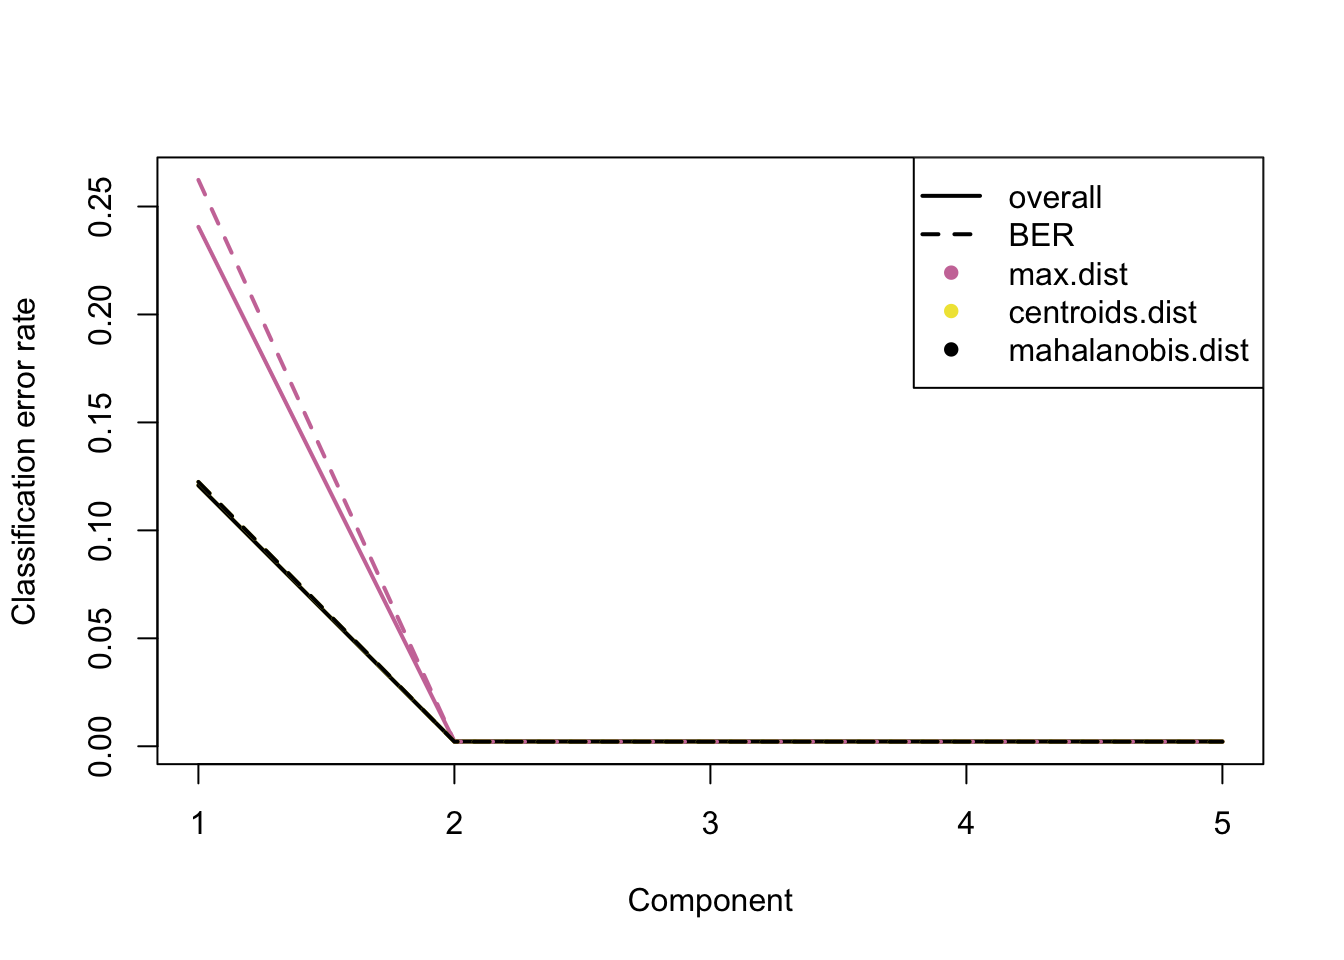
\includegraphics[width=0.55\linewidth]{MINT_Data_Integration_files/figure-latex/2-perfPlot10x-1} 

}

\caption{ The classification error rate for different number of PLSDA components of 10X dataset.}\label{fig:2-perfPlot10x}
\end{figure}

Similar to the combined dataset, \emph{ncomp}=2 leads to optimum error
rate. We now apply \emph{plsda} to the other 2 datasets:

\begin{Shaded}
\begin{Highlighting}[]
\CommentTok{## extract the normalised count matrix from the SCE object (transposed)}
\CommentTok{## CEL-seq2}
\NormalTok{normalised.cel =}\StringTok{ }\KeywordTok{t}\NormalTok{(}\KeywordTok{logcounts}\NormalTok{(sccel.norm))}
\NormalTok{normalised.cel =}\StringTok{ }\NormalTok{normalised.cel[,list.intersect]}
\CommentTok{## Drop-seq}
\NormalTok{normalised.drop=}\StringTok{ }\KeywordTok{t}\NormalTok{(}\KeywordTok{logcounts}\NormalTok{(scdrop.norm))}
\NormalTok{normalised.drop =}\StringTok{ }\NormalTok{normalised.drop[,list.intersect]}
\CommentTok{## factor variable of cell lines}
\NormalTok{Y.cel =}\StringTok{ }\KeywordTok{as.factor}\NormalTok{(sccel.norm[list.intersect,]}\OperatorTok{$}\NormalTok{cell_line)}
\NormalTok{Y.drop =}\StringTok{ }\KeywordTok{as.factor}\NormalTok{(scdrop.norm[list.intersect,]}\OperatorTok{$}\NormalTok{cell_line)}
\CommentTok{## PLS-DA on each dataset with 2 components}
\NormalTok{plsda}\FloatTok{.10}\NormalTok{x.res =}\StringTok{ }\KeywordTok{plsda}\NormalTok{(}\DataTypeTok{X =}\NormalTok{ normalised}\FloatTok{.10}\NormalTok{x, }\DataTypeTok{Y =}\NormalTok{ Y}\FloatTok{.10}\NormalTok{x, }\DataTypeTok{ncomp =} \DecValTok{2}\NormalTok{)}
\NormalTok{plsda.cel.res =}\StringTok{ }\KeywordTok{plsda}\NormalTok{(}\DataTypeTok{X =}\NormalTok{ normalised.cel, }\DataTypeTok{Y =}\NormalTok{ Y.cel, }\DataTypeTok{ncomp =} \DecValTok{2}\NormalTok{)}
\NormalTok{plsda.drop.res =}\StringTok{ }\KeywordTok{plsda}\NormalTok{(}\DataTypeTok{X =}\NormalTok{ normalised.drop, }\DataTypeTok{Y =}\NormalTok{ Y.drop, }\DataTypeTok{ncomp =} \DecValTok{2}\NormalTok{)}
\end{Highlighting}
\end{Shaded}

We plot the plsda plots for the 10X and CEL-seq2 data:

\begin{Shaded}
\begin{Highlighting}[]
\CommentTok{## mint.plsda plot for 10X}
\KeywordTok{plotIndiv}\NormalTok{(plsda}\FloatTok{.10}\NormalTok{x.res,}
          \DataTypeTok{legend  =} \OtherTok{TRUE}\NormalTok{, }\DataTypeTok{title     =} \StringTok{'PLSDA 10X'}\NormalTok{, }
          \DataTypeTok{ellipse =} \OtherTok{TRUE}\NormalTok{, }\DataTypeTok{legend.title =} \StringTok{'Cell Line'}\NormalTok{,}
          \DataTypeTok{X.label =} \StringTok{'PLSDA component 1'}\NormalTok{, }
          \DataTypeTok{Y.label =} \StringTok{'PLSDA component 2'}\NormalTok{, }\DataTypeTok{pch=}\DecValTok{1}\NormalTok{)}
\end{Highlighting}
\end{Shaded}

\begin{figure}[ht]

{\centering 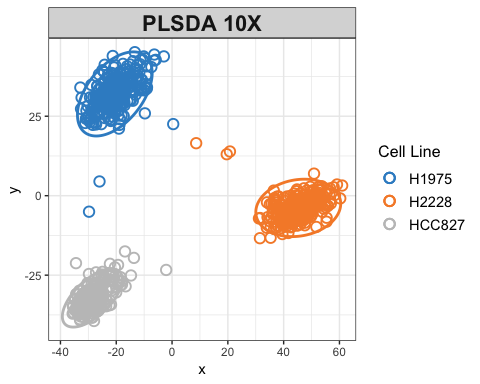
\includegraphics[width=0.65\linewidth]{MINT_Data_Integration_files/figure-latex/2-MINTplots-1} 

}

\caption{PLSDA plot for the 10x dataset.}\label{fig:2-MINTplots}
\end{figure}

\begin{Shaded}
\begin{Highlighting}[]
\CommentTok{## mint.plsda plot for CEL-seq2}
\KeywordTok{plotIndiv}\NormalTok{(plsda.cel.res,}
          \DataTypeTok{legend  =} \OtherTok{TRUE}\NormalTok{, }\DataTypeTok{title     =} \StringTok{'PLSDA CEL-seq2'}\NormalTok{, }
          \DataTypeTok{ellipse =} \OtherTok{TRUE}\NormalTok{, }\DataTypeTok{legend.title =} \StringTok{'Cell Line'}\NormalTok{,}
          \DataTypeTok{X.label =} \StringTok{'PLSDA component 1'}\NormalTok{, }
          \DataTypeTok{Y.label =} \StringTok{'PLSDA component 2'}\NormalTok{, }\DataTypeTok{pch=}\DecValTok{2}\NormalTok{)}
\end{Highlighting}
\end{Shaded}

\begin{figure}[ht]

{\centering 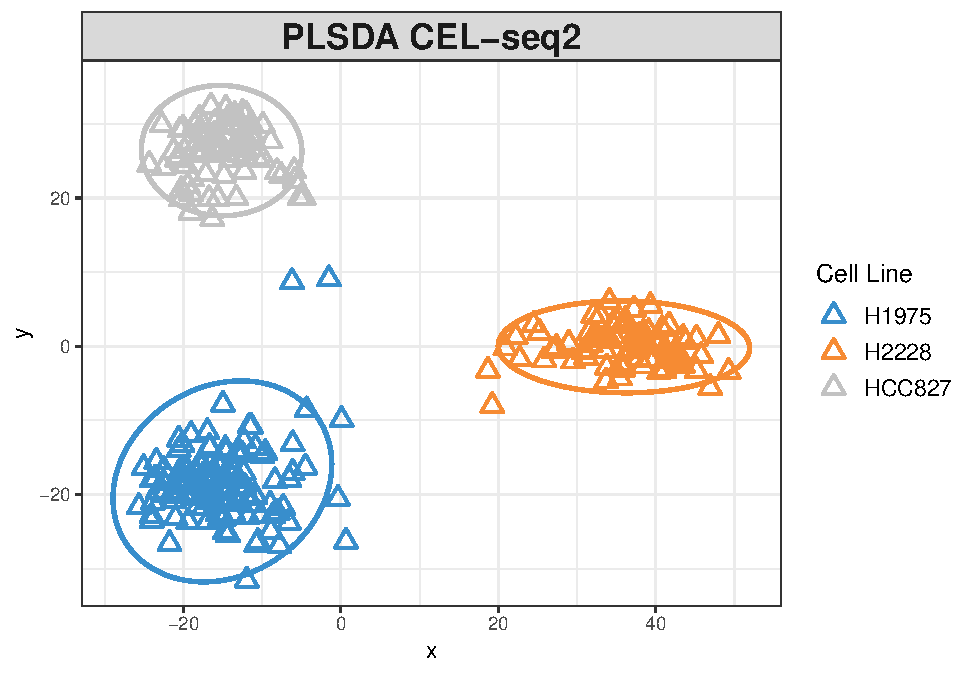
\includegraphics[width=0.65\linewidth]{MINT_Data_Integration_files/figure-latex/2-MINTplots2-1} 

}

\caption{PLSDA plot for the CEL-seq2 dataset.}\label{fig:2-MINTplots2}
\end{figure}

The PLSDA figures show clustering by cell line, while the CEL-seq2 data
are more scattered compared to 10X. In interpreting the relations, it is
important to note that the apparent change of clusters is simply the
result of an inversion on second PLSDA component and does not imply
disparity per se.

\hypertarget{sparse-plsda-splsda-for-each-protocol}{%
\subsection{Sparse PLSDA (sPLSDA) For Each
Protocol}\label{sparse-plsda-splsda-for-each-protocol}}

For consistency and better comparison, we will use same number of
optimum components as MINT for the sparse PLS-DA on each protocol:

\begin{Shaded}
\begin{Highlighting}[]
\CommentTok{## run sparse PLSDA on individual studies with MINT tuned parameters}
\NormalTok{keepX =}\StringTok{ }\KeywordTok{c}\NormalTok{(}\DecValTok{35}\NormalTok{,}\DecValTok{10}\NormalTok{)}
\NormalTok{splsda}\FloatTok{.10}\NormalTok{x.res =}\StringTok{ }\KeywordTok{splsda}\NormalTok{( }\DataTypeTok{X =}\NormalTok{normalised}\FloatTok{.10}\NormalTok{x, }\DataTypeTok{Y =}\NormalTok{ Y}\FloatTok{.10}\NormalTok{x, }\DataTypeTok{ncomp =} \DecValTok{2}\NormalTok{,  }
                              \DataTypeTok{keepX =}\NormalTok{ keepX)}
\NormalTok{splsda.cel.res =}\StringTok{ }\KeywordTok{splsda}\NormalTok{( }\DataTypeTok{X =}\NormalTok{normalised.cel, }\DataTypeTok{Y =}\NormalTok{ Y.cel, }\DataTypeTok{ncomp =} \DecValTok{2}\NormalTok{,  }
                              \DataTypeTok{keepX =}\NormalTok{ keepX)}
\NormalTok{splsda.drop.res =}\StringTok{ }\KeywordTok{splsda}\NormalTok{( }\DataTypeTok{X =}\NormalTok{normalised.drop, }\DataTypeTok{Y =}\NormalTok{ Y.drop, }\DataTypeTok{ncomp =} \DecValTok{2}\NormalTok{,  }
                              \DataTypeTok{keepX =}\NormalTok{ keepX)}
\end{Highlighting}
\end{Shaded}

And visualise the output to see how the clusters change with variable
selection:

\begin{Shaded}
\begin{Highlighting}[]
\CommentTok{## splsda plots with tuned number of variables for each sPLSDA component}
\CommentTok{## 10X}
\KeywordTok{plotIndiv}\NormalTok{(splsda}\FloatTok{.10}\NormalTok{x.res, }\DataTypeTok{group =}\NormalTok{ Y}\FloatTok{.10}\NormalTok{x,}
          \DataTypeTok{legend  =} \OtherTok{TRUE}\NormalTok{, }\DataTypeTok{title     =} \StringTok{'sPLSDA - 10X'}\NormalTok{,}
          \DataTypeTok{ellipse =} \OtherTok{FALSE}\NormalTok{,}\DataTypeTok{legend.title =} \StringTok{'Cell Line'}\NormalTok{,}
          \DataTypeTok{pch=}\DecValTok{1}\NormalTok{,}
          \DataTypeTok{X.label =} \StringTok{'sPLSDA component 1'}\NormalTok{,}
          \DataTypeTok{Y.label =} \StringTok{'sPLSDA component 2'}\NormalTok{)}
\end{Highlighting}
\end{Shaded}

\begin{figure}[ht]

{\centering 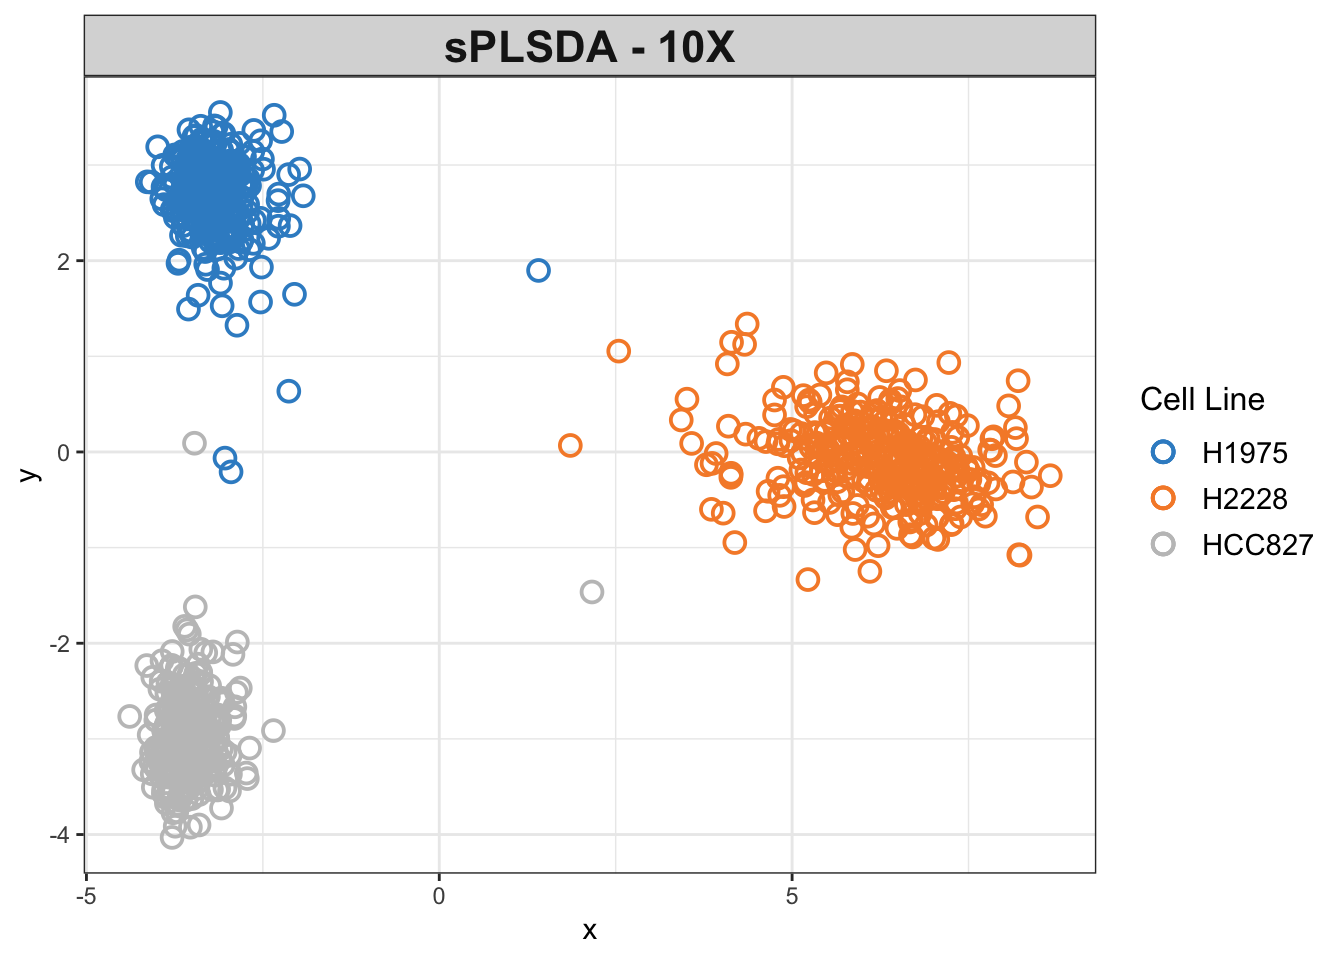
\includegraphics[width=0.65\linewidth]{MINT_Data_Integration_files/figure-latex/2-splsdaPlots1-1} 

}

\caption{ The sPLSDA plots of the 10X dataset.}\label{fig:2-splsdaPlots1}
\end{figure}

\begin{Shaded}
\begin{Highlighting}[]
\CommentTok{## CEL-seq2}
\KeywordTok{plotIndiv}\NormalTok{(splsda.cel.res, }\DataTypeTok{group =}\NormalTok{ Y.cel,}
          \DataTypeTok{legend  =} \OtherTok{TRUE}\NormalTok{, }\DataTypeTok{title     =} \StringTok{'sPLSDA - CEL-seq2'}\NormalTok{,}
          \DataTypeTok{ellipse =} \OtherTok{FALSE}\NormalTok{,}\DataTypeTok{legend.title =} \StringTok{'Cell Line'}\NormalTok{,}
          \DataTypeTok{pch=}\DecValTok{2}\NormalTok{,}
          \DataTypeTok{X.label =} \StringTok{'sPLSDA component 1'}\NormalTok{,}
          \DataTypeTok{Y.label =} \StringTok{'sPLSDA component 2'}\NormalTok{)}
\end{Highlighting}
\end{Shaded}

\begin{figure}[ht]

{\centering 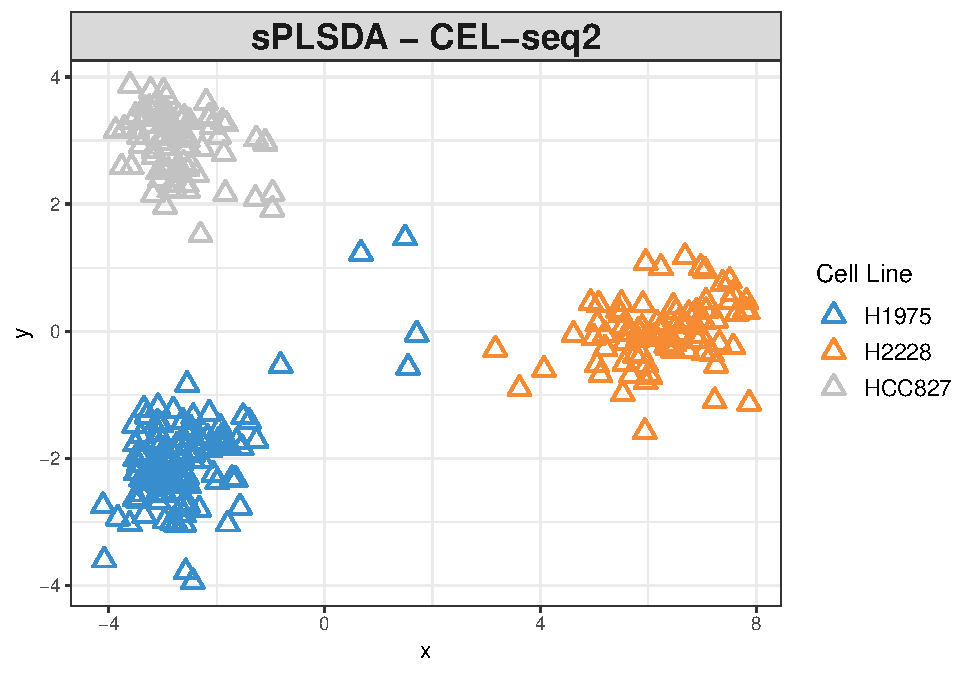
\includegraphics[width=0.65\linewidth]{MINT_Data_Integration_files/figure-latex/2-splsdaPlots2-1} 

}

\caption{ The sPLSDA plots of the CEL-seq2 dataset.}\label{fig:2-splsdaPlots2}
\end{figure}

The variable selection has reduced the noise and refined the clusters
compared to the non-sparse model.

\begin{Shaded}
\begin{Highlighting}[]
\CommentTok{## The signature genes from each sPLS-DA study}
\NormalTok{Chromium}\FloatTok{.10}\NormalTok{X.vars =}\StringTok{ }\KeywordTok{unique}\NormalTok{(}\KeywordTok{c}\NormalTok{(}\KeywordTok{selectVar}\NormalTok{(splsda}\FloatTok{.10}\NormalTok{x.res, }\DataTypeTok{comp=}\DecValTok{1}\NormalTok{)}\OperatorTok{$}\NormalTok{name,}
                             \KeywordTok{selectVar}\NormalTok{(splsda}\FloatTok{.10}\NormalTok{x.res, }\DataTypeTok{comp=}\DecValTok{2}\NormalTok{)}\OperatorTok{$}\NormalTok{name))}
\NormalTok{Cel.seq.vars =}\StringTok{      }\KeywordTok{unique}\NormalTok{(}\KeywordTok{c}\NormalTok{(}\KeywordTok{selectVar}\NormalTok{(splsda.cel.res, }\DataTypeTok{comp=}\DecValTok{1}\NormalTok{)}\OperatorTok{$}\NormalTok{name,}
                             \KeywordTok{selectVar}\NormalTok{(splsda.cel.res, }\DataTypeTok{comp=}\DecValTok{2}\NormalTok{)}\OperatorTok{$}\NormalTok{name))}
\NormalTok{Drop.seq.vars =}\StringTok{     }\KeywordTok{unique}\NormalTok{(}\KeywordTok{c}\NormalTok{(}\KeywordTok{selectVar}\NormalTok{(splsda.drop.res, }\DataTypeTok{comp=}\DecValTok{1}\NormalTok{)}\OperatorTok{$}\NormalTok{name,}
                             \KeywordTok{selectVar}\NormalTok{(splsda.drop.res, }\DataTypeTok{comp=}\DecValTok{2}\NormalTok{)}\OperatorTok{$}\NormalTok{name))}
\end{Highlighting}
\end{Shaded}

\begin{Shaded}
\begin{Highlighting}[]
\CommentTok{## create a venn diagram from signatures}
\NormalTok{vennProtocols <-}\StringTok{ }\KeywordTok{venn.diagram}\NormalTok{(}
    \DataTypeTok{x =} \KeywordTok{list}\NormalTok{(}
        \DataTypeTok{Chr.10X=}\NormalTok{ Chromium}\FloatTok{.10}\NormalTok{X.vars ,}
        \DataTypeTok{Cel.seq=}\NormalTok{ Cel.seq.vars,}
        \DataTypeTok{Drop.seq =}\NormalTok{ Drop.seq.vars),}
    \DataTypeTok{filename =} \OtherTok{NULL}\NormalTok{,}
    \DataTypeTok{cex=}\FloatTok{1.5}\NormalTok{, }\DataTypeTok{cat.cex=}\FloatTok{1.5}\NormalTok{,}
    \DataTypeTok{fill =} \KeywordTok{c}\NormalTok{(}\StringTok{'green'}\NormalTok{, }\StringTok{'darkblue'}\NormalTok{,  }\StringTok{'yellow'}\NormalTok{)}
\NormalTok{    )}
\KeywordTok{png}\NormalTok{(}\DataTypeTok{filename =} \StringTok{'figures/vennProtocols.png'}\NormalTok{)}
\KeywordTok{grid.draw}\NormalTok{(vennProtocols)}
\KeywordTok{dev.off}\NormalTok{()}
\end{Highlighting}
\end{Shaded}

\begin{figure}[ht]

{\centering 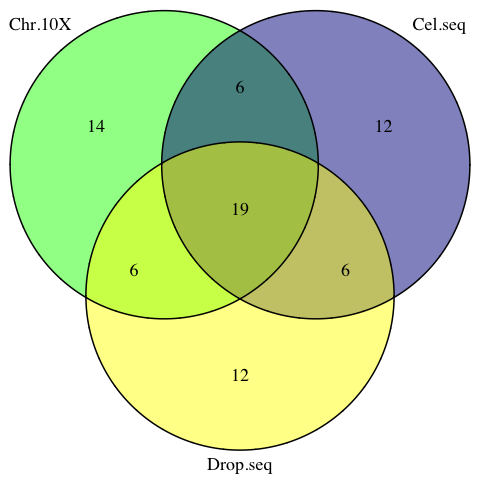
\includegraphics[width=0.35\linewidth]{figures/vennProtocols} 

}

\caption{ The venn diagram of common sPLSDA signatures among individual datasets.}\label{fig:2-vennProtocolsShow}
\end{figure}

The signatures from the 3 studies share 25 common genes.

\hypertarget{compare-with-mint-combined}{%
\section{Compare with MINT-Combined}\label{compare-with-mint-combined}}

In case the vignette is being run separately, the MINT sPLSDA object can
be reproduced:

Or directly from your local directory:

\hypertarget{loading-plots}{%
\subsection{Loading Plots}\label{loading-plots}}

The consistency of the selected variables across individual and the MINT
combined studies can be evaluated by plotting the loadings for each
study using the \emph{plotLoadings} function, which produces the barplot
of variable loadings for each component.

The inputs to \emph{plotLoadings} depends on the analysis object
(mint.\emph{s}plsda, mint.pls, etc.) and consists of the plot object
plus:

\begin{itemize}
\tightlist
\item
  \textbf{contrib:} Whether to show the class in which the expression of
  the features is maximum or minimum. One of \emph{`min'} or
  \emph{`max'}.
\item
  \textbf{method:} The criterion to assess the contribution. One of
  \emph{`mean'} or \emph{`median'} (recommended for skewed data).
\item
  \textbf{study:} The studies to be plotted (for combined data).
  \emph{all.partial} or \emph{global} for all.
\end{itemize}

For a complete list of the arguments for any object please refer to the
documentation.

We plot the loadings for both components for maximum contribution.
Colours indicate the class (cell line) in which the gene is
positively/negatively expressed:

\begin{Shaded}
\begin{Highlighting}[]
\CommentTok{## 10X}
\KeywordTok{plotLoadings}\NormalTok{(splsda}\FloatTok{.10}\NormalTok{x.res, }\DataTypeTok{contrib=}\StringTok{'max'}\NormalTok{, }\DataTypeTok{method =} \StringTok{'mean'}\NormalTok{, }\DataTypeTok{comp=}\DecValTok{1}\NormalTok{, }
             \DataTypeTok{study=}\StringTok{'all.partial'}\NormalTok{, }\DataTypeTok{legend=}\OtherTok{FALSE}\NormalTok{, }\DataTypeTok{title=}\OtherTok{NULL}\NormalTok{, }
             \DataTypeTok{subtitle =} \StringTok{'10X'}\NormalTok{)}
\end{Highlighting}
\end{Shaded}

\begin{figure}[ht]

{\centering 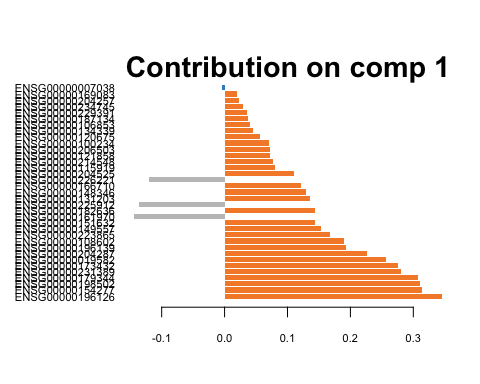
\includegraphics[width=0.55\linewidth]{MINT_Data_Integration_files/figure-latex/2-loadings1-1} 

}

\caption{The loading plots for the first component of sPLS-DA on 10X data. The orange colour corresponds to H2228 cells, and the grey colour belongs to HCC827 cell line.}\label{fig:2-loadings1}
\end{figure}

\begin{Shaded}
\begin{Highlighting}[]
\CommentTok{## CEL-seq2}
\KeywordTok{plotLoadings}\NormalTok{(splsda.cel.res, }\DataTypeTok{contrib=}\StringTok{'max'}\NormalTok{, }\DataTypeTok{method =} \StringTok{'mean'}\NormalTok{, }\DataTypeTok{comp=}\DecValTok{1}\NormalTok{, }
             \DataTypeTok{study=}\StringTok{'all.partial'}\NormalTok{, }\DataTypeTok{legend=}\OtherTok{FALSE}\NormalTok{, }\DataTypeTok{title=}\OtherTok{NULL}\NormalTok{,}
             \DataTypeTok{subtitle =} \StringTok{'CEL-seq2'}\NormalTok{)}
\end{Highlighting}
\end{Shaded}

\begin{figure}[ht]

{\centering 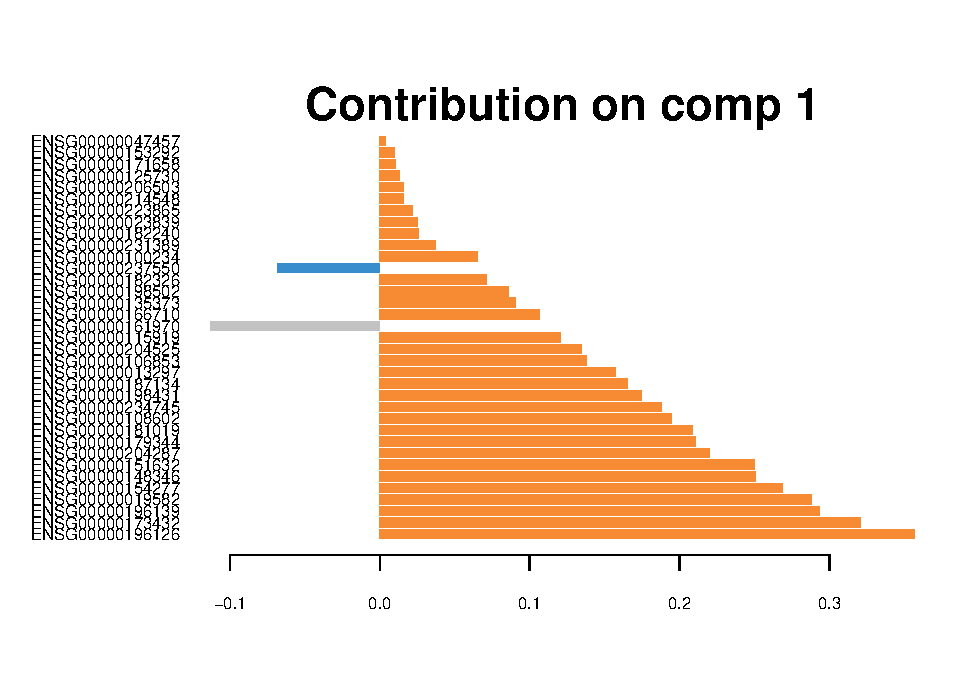
\includegraphics[width=0.55\linewidth]{MINT_Data_Integration_files/figure-latex/2-loadings2-1} 

}

\caption{The loading plots for the first component of sPLS-DA on CEL-seq2 data.}\label{fig:2-loadings2}
\end{figure}

\begin{Shaded}
\begin{Highlighting}[]
\CommentTok{## Drop-seq}
\KeywordTok{plotLoadings}\NormalTok{(splsda.drop.res, }\DataTypeTok{contrib=}\StringTok{'max'}\NormalTok{, }\DataTypeTok{method =} \StringTok{'mean'}\NormalTok{, }\DataTypeTok{comp=}\DecValTok{1}\NormalTok{, }
             \DataTypeTok{study=}\StringTok{'all.partial'}\NormalTok{, }\DataTypeTok{legend=}\OtherTok{FALSE}\NormalTok{, }\DataTypeTok{title=}\OtherTok{NULL}\NormalTok{,}
             \DataTypeTok{subtitle =} \StringTok{'Drop-seq'}\NormalTok{)}
\end{Highlighting}
\end{Shaded}

\begin{figure}[ht]

{\centering 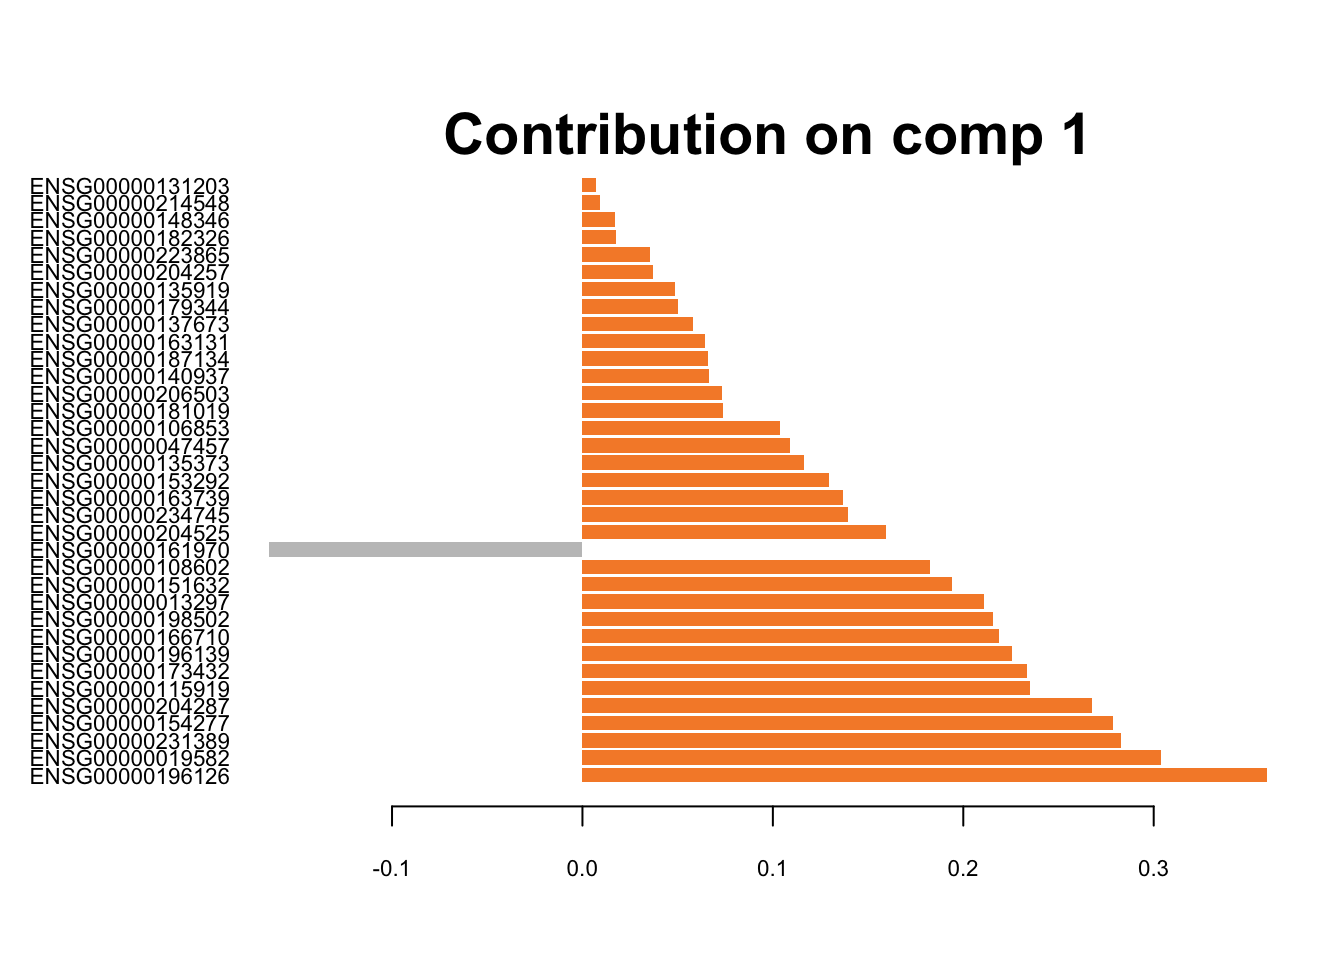
\includegraphics[width=0.55\linewidth]{MINT_Data_Integration_files/figure-latex/2-loadings3-1} 

}

\caption{The loading plots for the first component of sPLS-DA on Drop-seq data.}\label{fig:2-loadings3}
\end{figure}

These genes are differentiating cells along the first sPLSDA component.
Majority of signature genes are postively expressed in H2228 cells
(orange). There is not a clear consensus among individual datasets in
terms of the signature genes and their weight (loading).

\begin{Shaded}
\begin{Highlighting}[]
\CommentTok{## MINT Comp. 1}
\KeywordTok{plotLoadings}\NormalTok{(mint.splsda.res, }\DataTypeTok{contrib=}\StringTok{'max'}\NormalTok{, }\DataTypeTok{method =} \StringTok{'mean'}\NormalTok{, }\DataTypeTok{comp=}\DecValTok{1}\NormalTok{, }
             \DataTypeTok{study=}\StringTok{'all.partial'}\NormalTok{, }\DataTypeTok{legend=}\OtherTok{FALSE}\NormalTok{, }\DataTypeTok{title=}\OtherTok{NULL}\NormalTok{, }
             \DataTypeTok{subtitle =} \KeywordTok{c}\NormalTok{(}\StringTok{'10X'}\NormalTok{, }\StringTok{'CEL-seq2'}\NormalTok{, }\StringTok{'Drop-seq'}\NormalTok{) )}
\end{Highlighting}
\end{Shaded}

\begin{figure}[ht]

{\centering 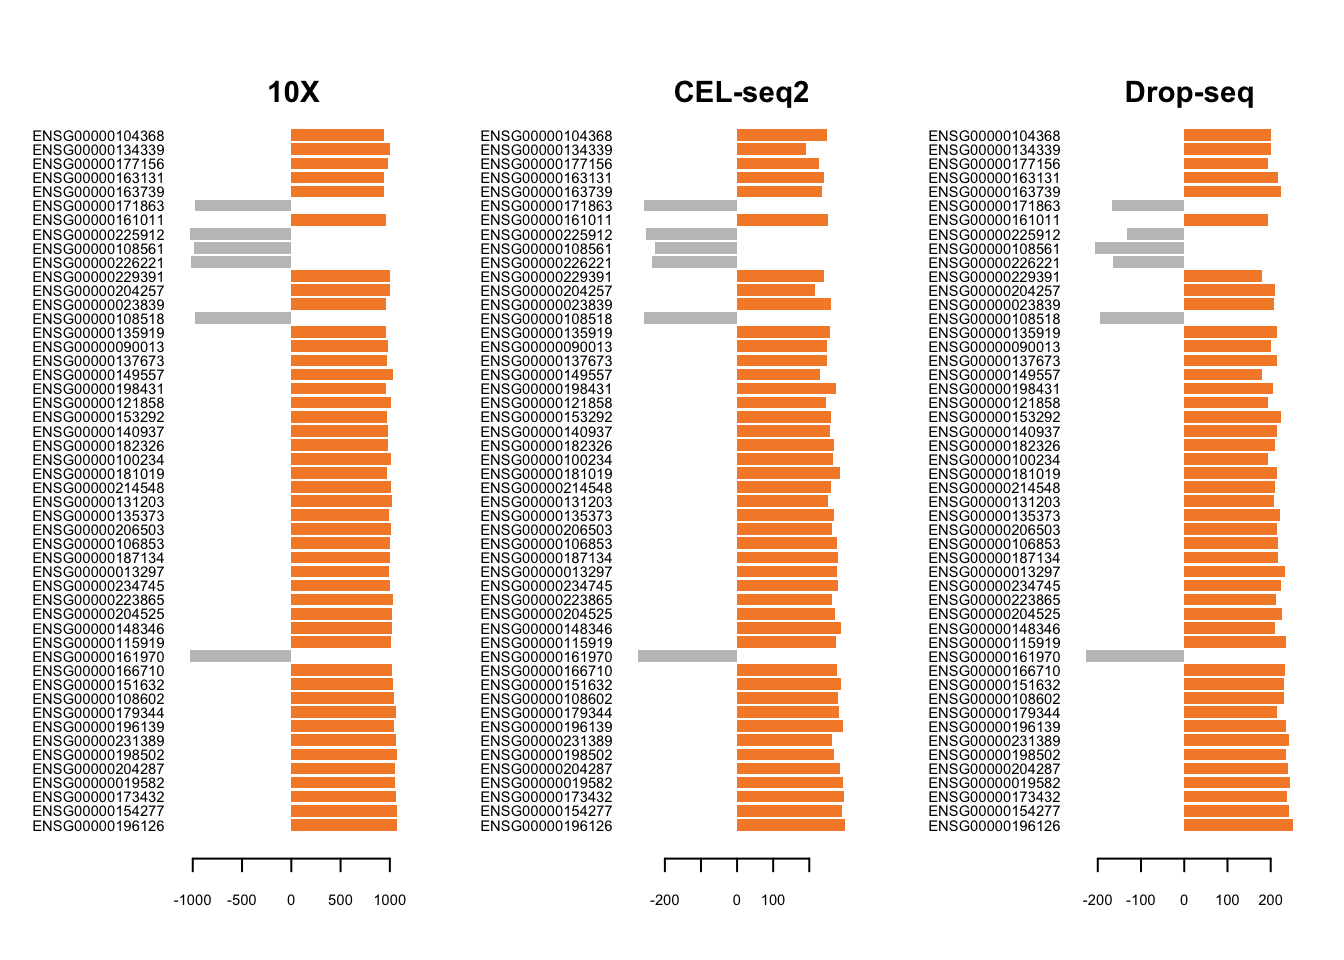
\includegraphics[width=0.65\linewidth]{MINT_Data_Integration_files/figure-latex/2-loadings4-1} 

}

\caption{The loading plots for the first component of the Sparse MINT on the combined dataset.}\label{fig:2-loadings4}
\end{figure}

MINT has produced signature that is consistent across studies.
Similarly, we can plot the loadings on the second component variables.

\begin{Shaded}
\begin{Highlighting}[]
\CommentTok{## MINT Comp. 2}
\KeywordTok{plotLoadings}\NormalTok{(mint.splsda.tuned.res, }\DataTypeTok{contrib=}\StringTok{'max'}\NormalTok{, }\DataTypeTok{method =} \StringTok{'mean'}\NormalTok{, }\DataTypeTok{comp=}\DecValTok{2}\NormalTok{, }
             \DataTypeTok{study=}\StringTok{'all.partial'}\NormalTok{, }\DataTypeTok{legend=}\OtherTok{FALSE}\NormalTok{, }\DataTypeTok{title=}\OtherTok{NULL}\NormalTok{, }
             \DataTypeTok{subtitle =} \KeywordTok{c}\NormalTok{(}\StringTok{'10X'}\NormalTok{, }\StringTok{'CEL-seq2'}\NormalTok{, }\StringTok{'Drop-seq'}\NormalTok{) )}
\end{Highlighting}
\end{Shaded}

\begin{figure}[ht]

{\centering 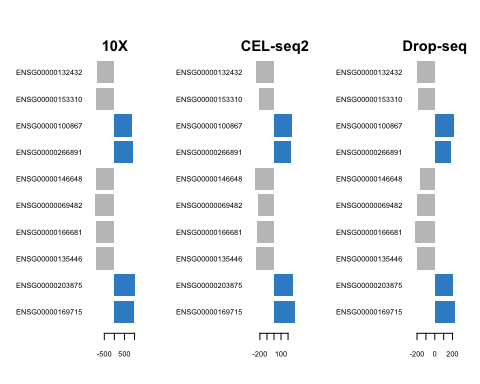
\includegraphics[width=0.65\linewidth]{MINT_Data_Integration_files/figure-latex/2-loadingscomp2-1} 

}

\caption{The loading plots for the second component of the Sparse MINT on the combined dataset.}\label{fig:2-loadingscomp2}
\end{figure}

\hypertarget{signature-comparison}{%
\subsection{Signature Comparison}\label{signature-comparison}}

The \emph{selectVar} function in \emph{mixOmics} outputs the key
predictors on each component along with their loadings. We can create a
set of Venn diagrams to visualise the overlap of the signature found
using PLS-DA in individual datasets and the combined dataset. For all
datasets, we take all the variables on both components as the signature.

\begin{Shaded}
\begin{Highlighting}[]
\CommentTok{## MINT signature}
\NormalTok{MINT.Combined.vars =}\StringTok{ }\KeywordTok{unique}\NormalTok{(}\KeywordTok{c}\NormalTok{(}\KeywordTok{selectVar}\NormalTok{(mint.splsda.tuned.res, }\DataTypeTok{comp=}\DecValTok{1}\NormalTok{)}\OperatorTok{$}\NormalTok{name,}
                             \KeywordTok{selectVar}\NormalTok{(mint.splsda.tuned.res, }\DataTypeTok{comp=}\DecValTok{2}\NormalTok{)}\OperatorTok{$}\NormalTok{name))}
\end{Highlighting}
\end{Shaded}

\begin{Shaded}
\begin{Highlighting}[]
\NormalTok{vennMINT <-}\StringTok{ }\KeywordTok{venn.diagram}\NormalTok{(}
    \DataTypeTok{x =} \KeywordTok{list}\NormalTok{(}
        \DataTypeTok{Chr.10X=}\NormalTok{ Chromium}\FloatTok{.10}\NormalTok{X.vars ,}
        \DataTypeTok{Cel.seq=}\NormalTok{ Cel.seq.vars,}
        \DataTypeTok{Drop.seq =}\NormalTok{ Drop.seq.vars,}
        \DataTypeTok{MINT.Combined=}\NormalTok{MINT.Combined.vars),}
    \DataTypeTok{filename =} \OtherTok{NULL}\NormalTok{,}
    \DataTypeTok{cex=}\FloatTok{1.5}\NormalTok{, }\DataTypeTok{cat.cex=}\FloatTok{1.5}\NormalTok{,}
    \DataTypeTok{fill =} \KeywordTok{c}\NormalTok{(}\StringTok{'green'}\NormalTok{, }\StringTok{'darkblue'}\NormalTok{,  }\StringTok{'yellow'}\NormalTok{, }\StringTok{'red'}\NormalTok{)}
\NormalTok{    )}
\KeywordTok{png}\NormalTok{(}\DataTypeTok{filename =} \StringTok{'figures/vennMINT.png'}\NormalTok{)}
\KeywordTok{grid.draw}\NormalTok{(vennMINT)}
\KeywordTok{dev.off}\NormalTok{()}
\end{Highlighting}
\end{Shaded}

\begin{figure}[ht]

{\centering 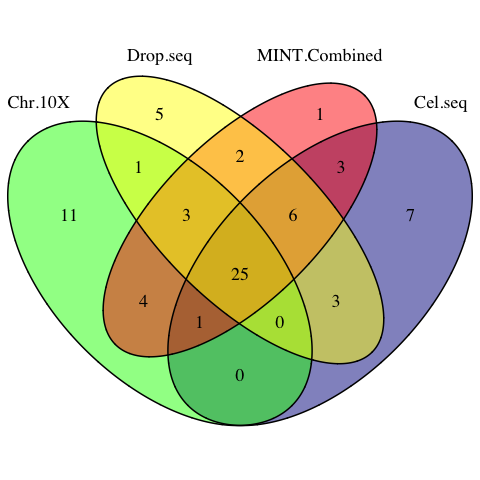
\includegraphics[width=0.55\linewidth]{figures/vennMINT} 

}

\caption{ The venn diagram of sPLSDA signatures among individual datasets and the MINT combined dataset.}\label{fig:2-vennMINTShow}
\end{figure}

\begin{Shaded}
\begin{Highlighting}[]
\CommentTok{## the signature genes identified by all studies}
\NormalTok{common.sig =}\StringTok{ }\KeywordTok{Reduce}\NormalTok{(intersect, }\KeywordTok{list}\NormalTok{(MINT.Combined.vars, Chromium}\FloatTok{.10}\NormalTok{X.vars, Cel.seq.vars, Drop.seq.vars))}
\end{Highlighting}
\end{Shaded}

MINT has successfully detected the core 25 signature genes shared by all
individual PLSDA models, plus 10 genes identied in 2 out of 3 studies.

\begin{Shaded}
\begin{Highlighting}[]
\CommentTok{## the 10 signature genes with highest loadings}
\NormalTok{common.sig[}\DecValTok{1}\OperatorTok{:}\DecValTok{10}\NormalTok{]}
\end{Highlighting}
\end{Shaded}

\begin{verbatim}
##  [1] "ENSG00000196126" "ENSG00000154277" "ENSG00000173432"
##  [4] "ENSG00000019582" "ENSG00000204287" "ENSG00000198502"
##  [7] "ENSG00000231389" "ENSG00000196139" "ENSG00000179344"
## [10] "ENSG00000108602"
\end{verbatim}

\hypertarget{variable-plots}{%
\subsection{Variable Plots}\label{variable-plots}}

Using \emph{plotVar} function, it is possible to display the selected
variables on a correlation circle plot to find the correlation between
gene expressions:

\begin{Shaded}
\begin{Highlighting}[]
\CommentTok{## correlation circle plot}
\KeywordTok{plotVar}\NormalTok{(mint.splsda.tuned.res, }\DataTypeTok{cex =} \DecValTok{3}\NormalTok{)}
\end{Highlighting}
\end{Shaded}

\begin{figure}[ht]

{\centering 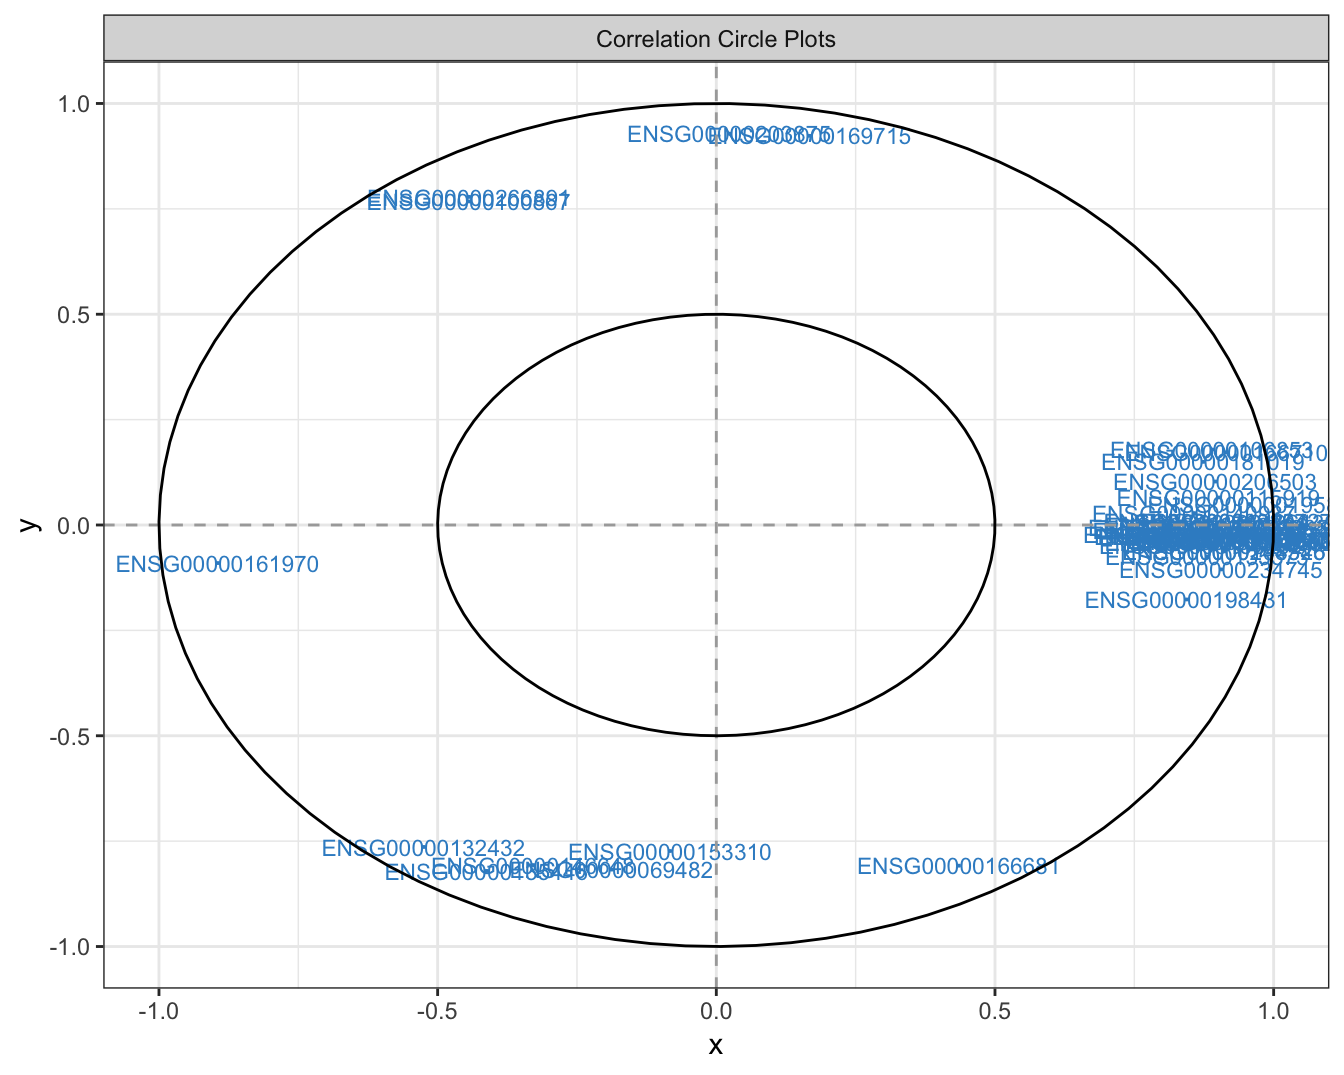
\includegraphics[width=0.55\linewidth]{MINT_Data_Integration_files/figure-latex/unnamed-chunk-7-1} 

}

\caption{The variable plot highlighting the contribution of each selected variable to each component and their correlation.}\label{fig:unnamed-chunk-7}
\end{figure}

The figure above shows that majority of the signature genes are
positively expressed in component 1.

we can assess the expression profiles for the genes on the extremes of
both components:

\begin{Shaded}
\begin{Highlighting}[]
\CommentTok{## component 1 - most positively and negatively expressed between cell lines}
\NormalTok{var.c1 =}\StringTok{ }\KeywordTok{selectVar}\NormalTok{(mint.splsda.tuned.res, }\DataTypeTok{comp=}\DecValTok{1}\NormalTok{)}\OperatorTok{$}\NormalTok{value}
\NormalTok{positive.gene.c1 =}\StringTok{ }\KeywordTok{rownames}\NormalTok{(var.c1)[}\KeywordTok{which.max}\NormalTok{(var.c1}\OperatorTok{$}\NormalTok{value.var)]}
\NormalTok{negative.gene.c1 =}\StringTok{ }\KeywordTok{rownames}\NormalTok{(var.c1)[}\KeywordTok{which.min}\NormalTok{(var.c1}\OperatorTok{$}\NormalTok{value.var)]}

\CommentTok{## component 2 - most positively and negatively expressed between cell lines}
\NormalTok{var.c2 =}\StringTok{ }\KeywordTok{selectVar}\NormalTok{(mint.splsda.tuned.res, }\DataTypeTok{comp=}\DecValTok{2}\NormalTok{)}\OperatorTok{$}\NormalTok{value}
\NormalTok{positive.gene.c2 =}\StringTok{ }\KeywordTok{rownames}\NormalTok{(var.c2)[}\KeywordTok{which.max}\NormalTok{(var.c2}\OperatorTok{$}\NormalTok{value.var)]}
\NormalTok{negative.gene.c2 =}\StringTok{ }\KeywordTok{rownames}\NormalTok{(var.c2)[}\KeywordTok{which.min}\NormalTok{(var.c2}\OperatorTok{$}\NormalTok{value.var)]}
\end{Highlighting}
\end{Shaded}

\begin{Shaded}
\begin{Highlighting}[]
\CommentTok{## a function to create violin + box plots for this specific dataset}
\NormalTok{violinPlot =}\StringTok{ }\ControlFlowTok{function}\NormalTok{(mint.object, gene)\{}
\NormalTok{  cols =}\StringTok{ }\KeywordTok{c}\NormalTok{(}\StringTok{"H2228"}\NormalTok{ =}\StringTok{ "orange"}\NormalTok{, }\StringTok{"H1975"}\NormalTok{ =}\StringTok{ "dodgerblue3"}\NormalTok{, }\StringTok{"HCC827"}\NormalTok{ =}\StringTok{ "grey"}\NormalTok{)}
  \KeywordTok{ggplot}\NormalTok{() }\OperatorTok{+}\StringTok{ }
\StringTok{    }\KeywordTok{geom_boxplot}\NormalTok{(}\KeywordTok{aes}\NormalTok{(mint.object}\OperatorTok{$}\NormalTok{Y,  mint.object}\OperatorTok{$}\NormalTok{X[,gene],}
                     \DataTypeTok{fill=}\NormalTok{ mint.object}\OperatorTok{$}\NormalTok{Y), }\DataTypeTok{alpha=}\DecValTok{1}\NormalTok{)}\OperatorTok{+}
\StringTok{    }\KeywordTok{geom_violin}\NormalTok{(}\KeywordTok{aes}\NormalTok{(mint.object}\OperatorTok{$}\NormalTok{Y, mint.object}\OperatorTok{$}\NormalTok{X[,gene],}
                     \DataTypeTok{fill=}\NormalTok{ mint.object}\OperatorTok{$}\NormalTok{Y), }\DataTypeTok{alpha=}\FloatTok{0.7}\NormalTok{) }\OperatorTok{+}
\StringTok{    }\KeywordTok{labs}\NormalTok{(}\DataTypeTok{x =} \StringTok{"Cell Line"}\NormalTok{, }\DataTypeTok{y=}\StringTok{"Standardised Expression Value"}\NormalTok{ )}\OperatorTok{+}
\StringTok{    }\KeywordTok{guides}\NormalTok{(}\DataTypeTok{fill=}\KeywordTok{guide_legend}\NormalTok{(}\DataTypeTok{title=}\StringTok{"Cell Line"}\NormalTok{) ) }\OperatorTok{+}
\StringTok{    }\KeywordTok{scale_fill_manual}\NormalTok{(}\DataTypeTok{values=}\NormalTok{cols ) }
\NormalTok{\}}
\end{Highlighting}
\end{Shaded}

\begin{Shaded}
\begin{Highlighting}[]
\CommentTok{## violin + box plots for the most positively expressed gene on component 1}
\KeywordTok{violinPlot}\NormalTok{(mint.splsda.tuned.res, positive.gene.c1)}
\end{Highlighting}
\end{Shaded}

\begin{figure}[ht]

{\centering 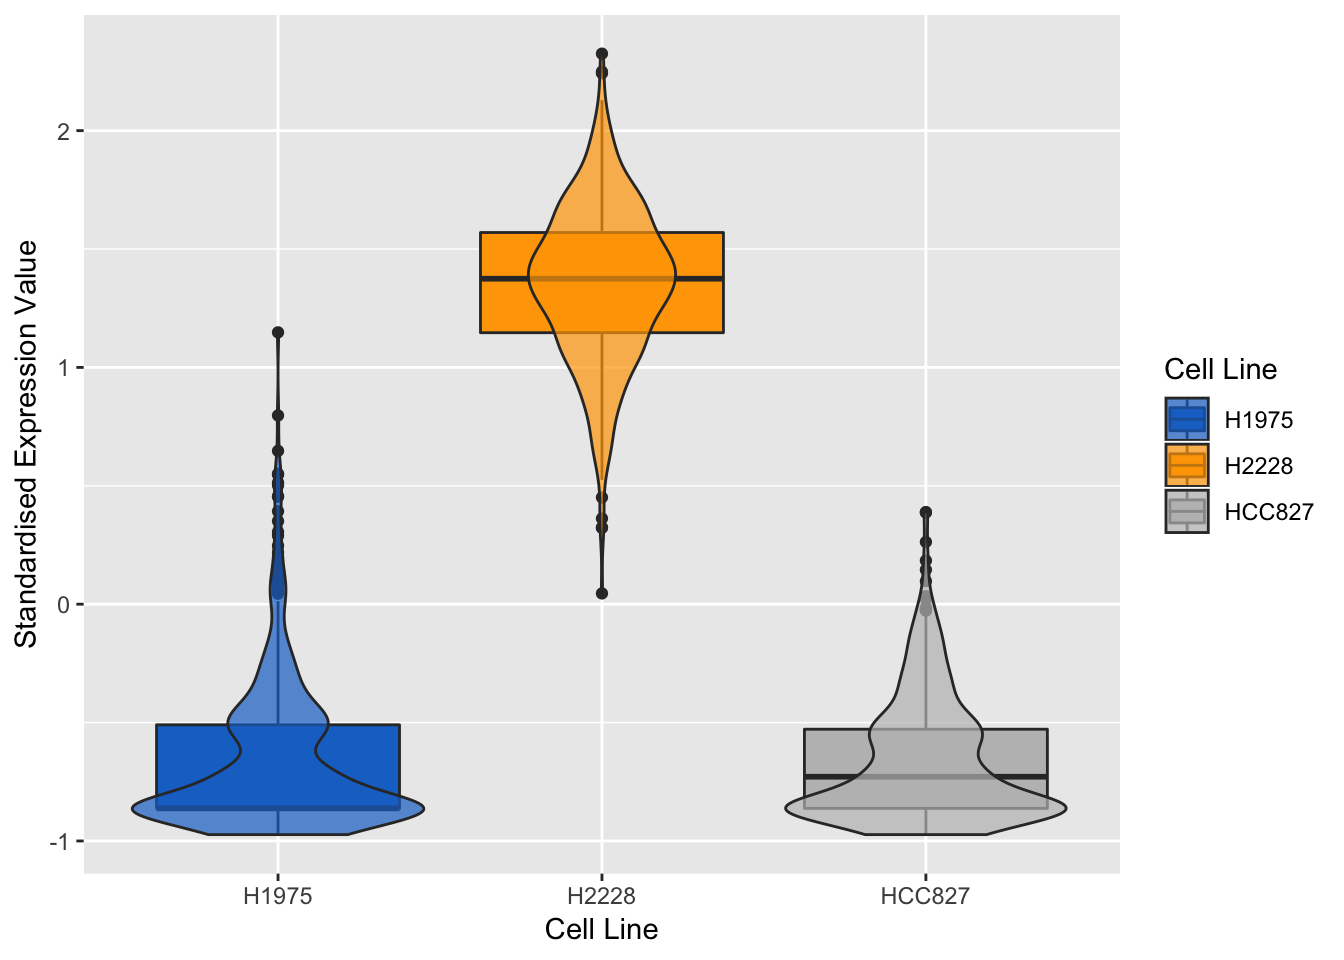
\includegraphics[width=0.5\linewidth]{MINT_Data_Integration_files/figure-latex/2-vilolinplotPositive-1} 

}

\caption{Violin plots of expression profile of the most positively expressed gene on component 1 in different cell lines}\label{fig:2-vilolinplotPositive}
\end{figure}

\begin{Shaded}
\begin{Highlighting}[]
\CommentTok{## violin + box plots for the most negatively expressed gene on component 1}
\KeywordTok{violinPlot}\NormalTok{(mint.splsda.tuned.res, negative.gene.c1)}
\end{Highlighting}
\end{Shaded}

\begin{figure}[ht]

{\centering 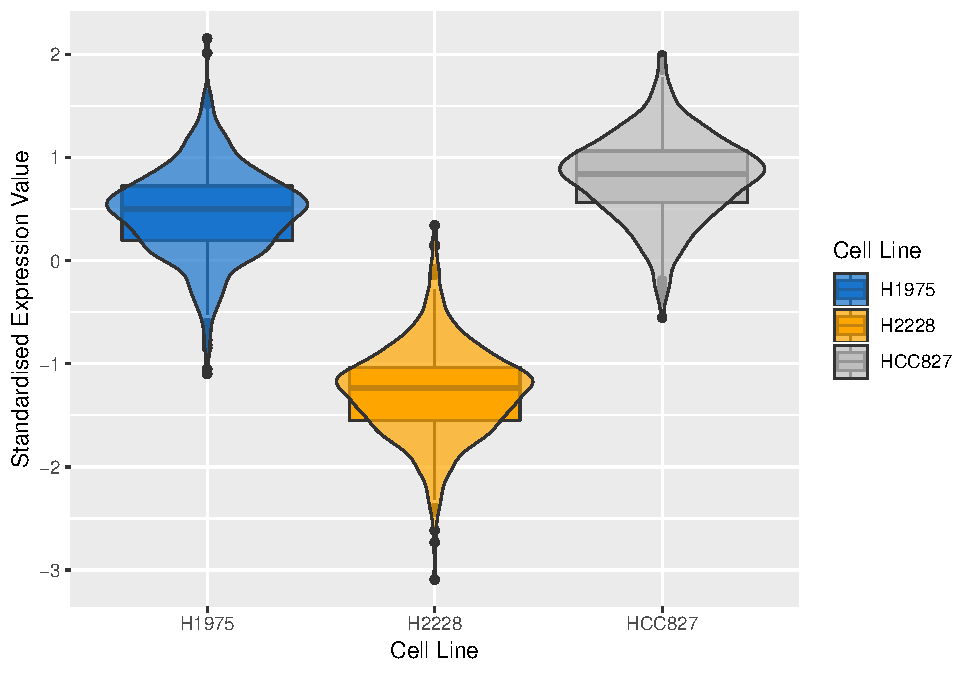
\includegraphics[width=0.5\linewidth]{MINT_Data_Integration_files/figure-latex/2-vilolinplotNegative-1} 

}

\caption{Violin plots of expression profile of the most negatively expressed gene  on component 1 in different cell lines}\label{fig:2-vilolinplotNegative}
\end{figure}

As expected, the expression profile of the above genes for H2228 cell
line has opposite correlation to the other two. We can also evaluate the
genes of the second sPLS-DA component:

\begin{Shaded}
\begin{Highlighting}[]
\CommentTok{## violin + box plots for the most positively expressed gene on component 2}
\KeywordTok{violinPlot}\NormalTok{(mint.splsda.tuned.res, positive.gene.c2)}
\end{Highlighting}
\end{Shaded}

\begin{figure}[ht]

{\centering 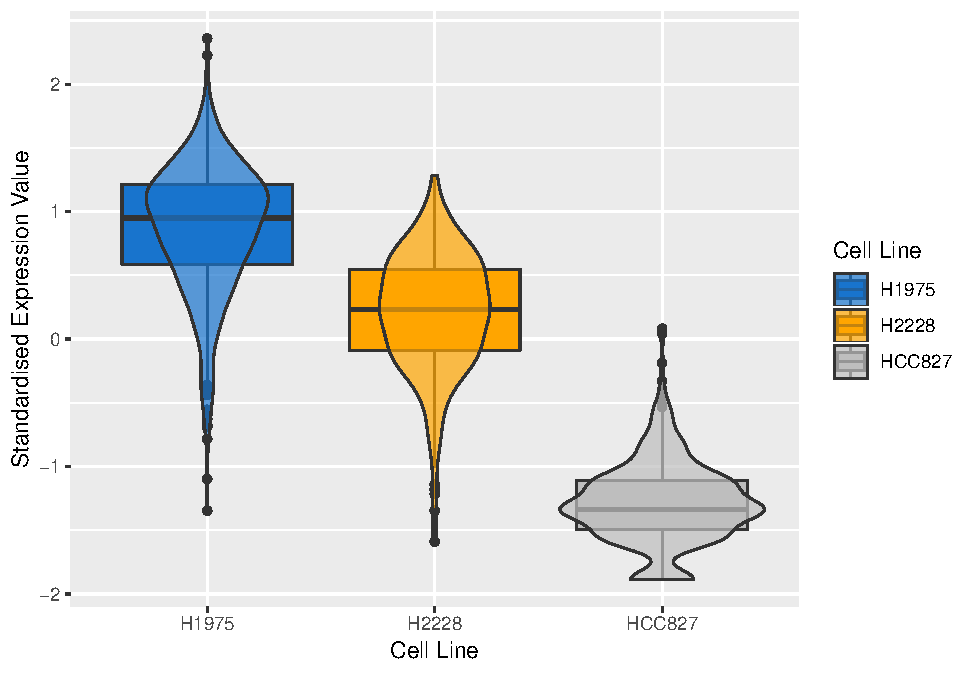
\includegraphics[width=0.5\linewidth]{MINT_Data_Integration_files/figure-latex/2-vilolinplotPositive-c2-1} 

}

\caption{Violin plots of expression profile of the most positively expressed gene on component 2 in different cell lines}\label{fig:2-vilolinplotPositive-c2}
\end{figure}

\begin{Shaded}
\begin{Highlighting}[]
\CommentTok{## violin + box plots for the most negatively expressed gene on component 2}
\KeywordTok{violinPlot}\NormalTok{(mint.splsda.tuned.res, negative.gene.c2)}
\end{Highlighting}
\end{Shaded}

\begin{figure}[ht]

{\centering 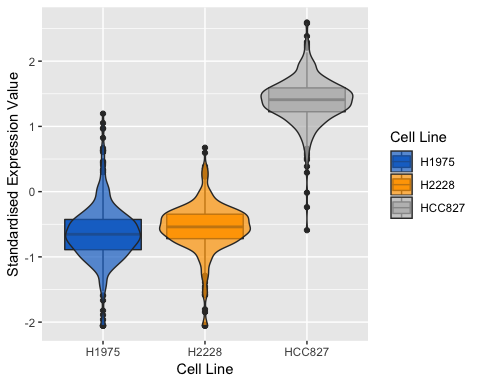
\includegraphics[width=0.5\linewidth]{MINT_Data_Integration_files/figure-latex/2-vilolinplotNegative-c2-1} 

}

\caption{Violin plots of expression profile of the most negatively expressed gene  on component 2 in different cell lines}\label{fig:2-vilolinplotNegative-c2}
\end{figure}

The expression profiles show that the selected gene tends to be
negatively expressed in HCC827 cell line and positively expressed in
H1975 cell line.

A Clustered Image Map including the final signature can be plotted. The
argument \emph{comp} can be also be specified to highlight only the
variables selected on specific components.

\begin{Shaded}
\begin{Highlighting}[]
\KeywordTok{cim}\NormalTok{(mint.splsda.tuned.res, }\DataTypeTok{comp =} \KeywordTok{c}\NormalTok{(}\DecValTok{1}\NormalTok{,}\DecValTok{2}\NormalTok{), }\DataTypeTok{margins=}\KeywordTok{c}\NormalTok{(}\DecValTok{10}\NormalTok{,}\DecValTok{5}\NormalTok{), }
    \DataTypeTok{row.sideColors =} \KeywordTok{color.mixo}\NormalTok{(}\KeywordTok{as.numeric}\NormalTok{(mint.splsda.tuned.res}\OperatorTok{$}\NormalTok{Y)), }\DataTypeTok{row.names =} \OtherTok{FALSE}\NormalTok{,}
    \DataTypeTok{title =} \StringTok{'MINT sPLS-DA'}\NormalTok{, }\DataTypeTok{save=}\StringTok{'png'}\NormalTok{, }\DataTypeTok{name.save =} \StringTok{'heatmap'}\NormalTok{)}
\end{Highlighting}
\end{Shaded}

\begin{figure}[ht]

{\centering 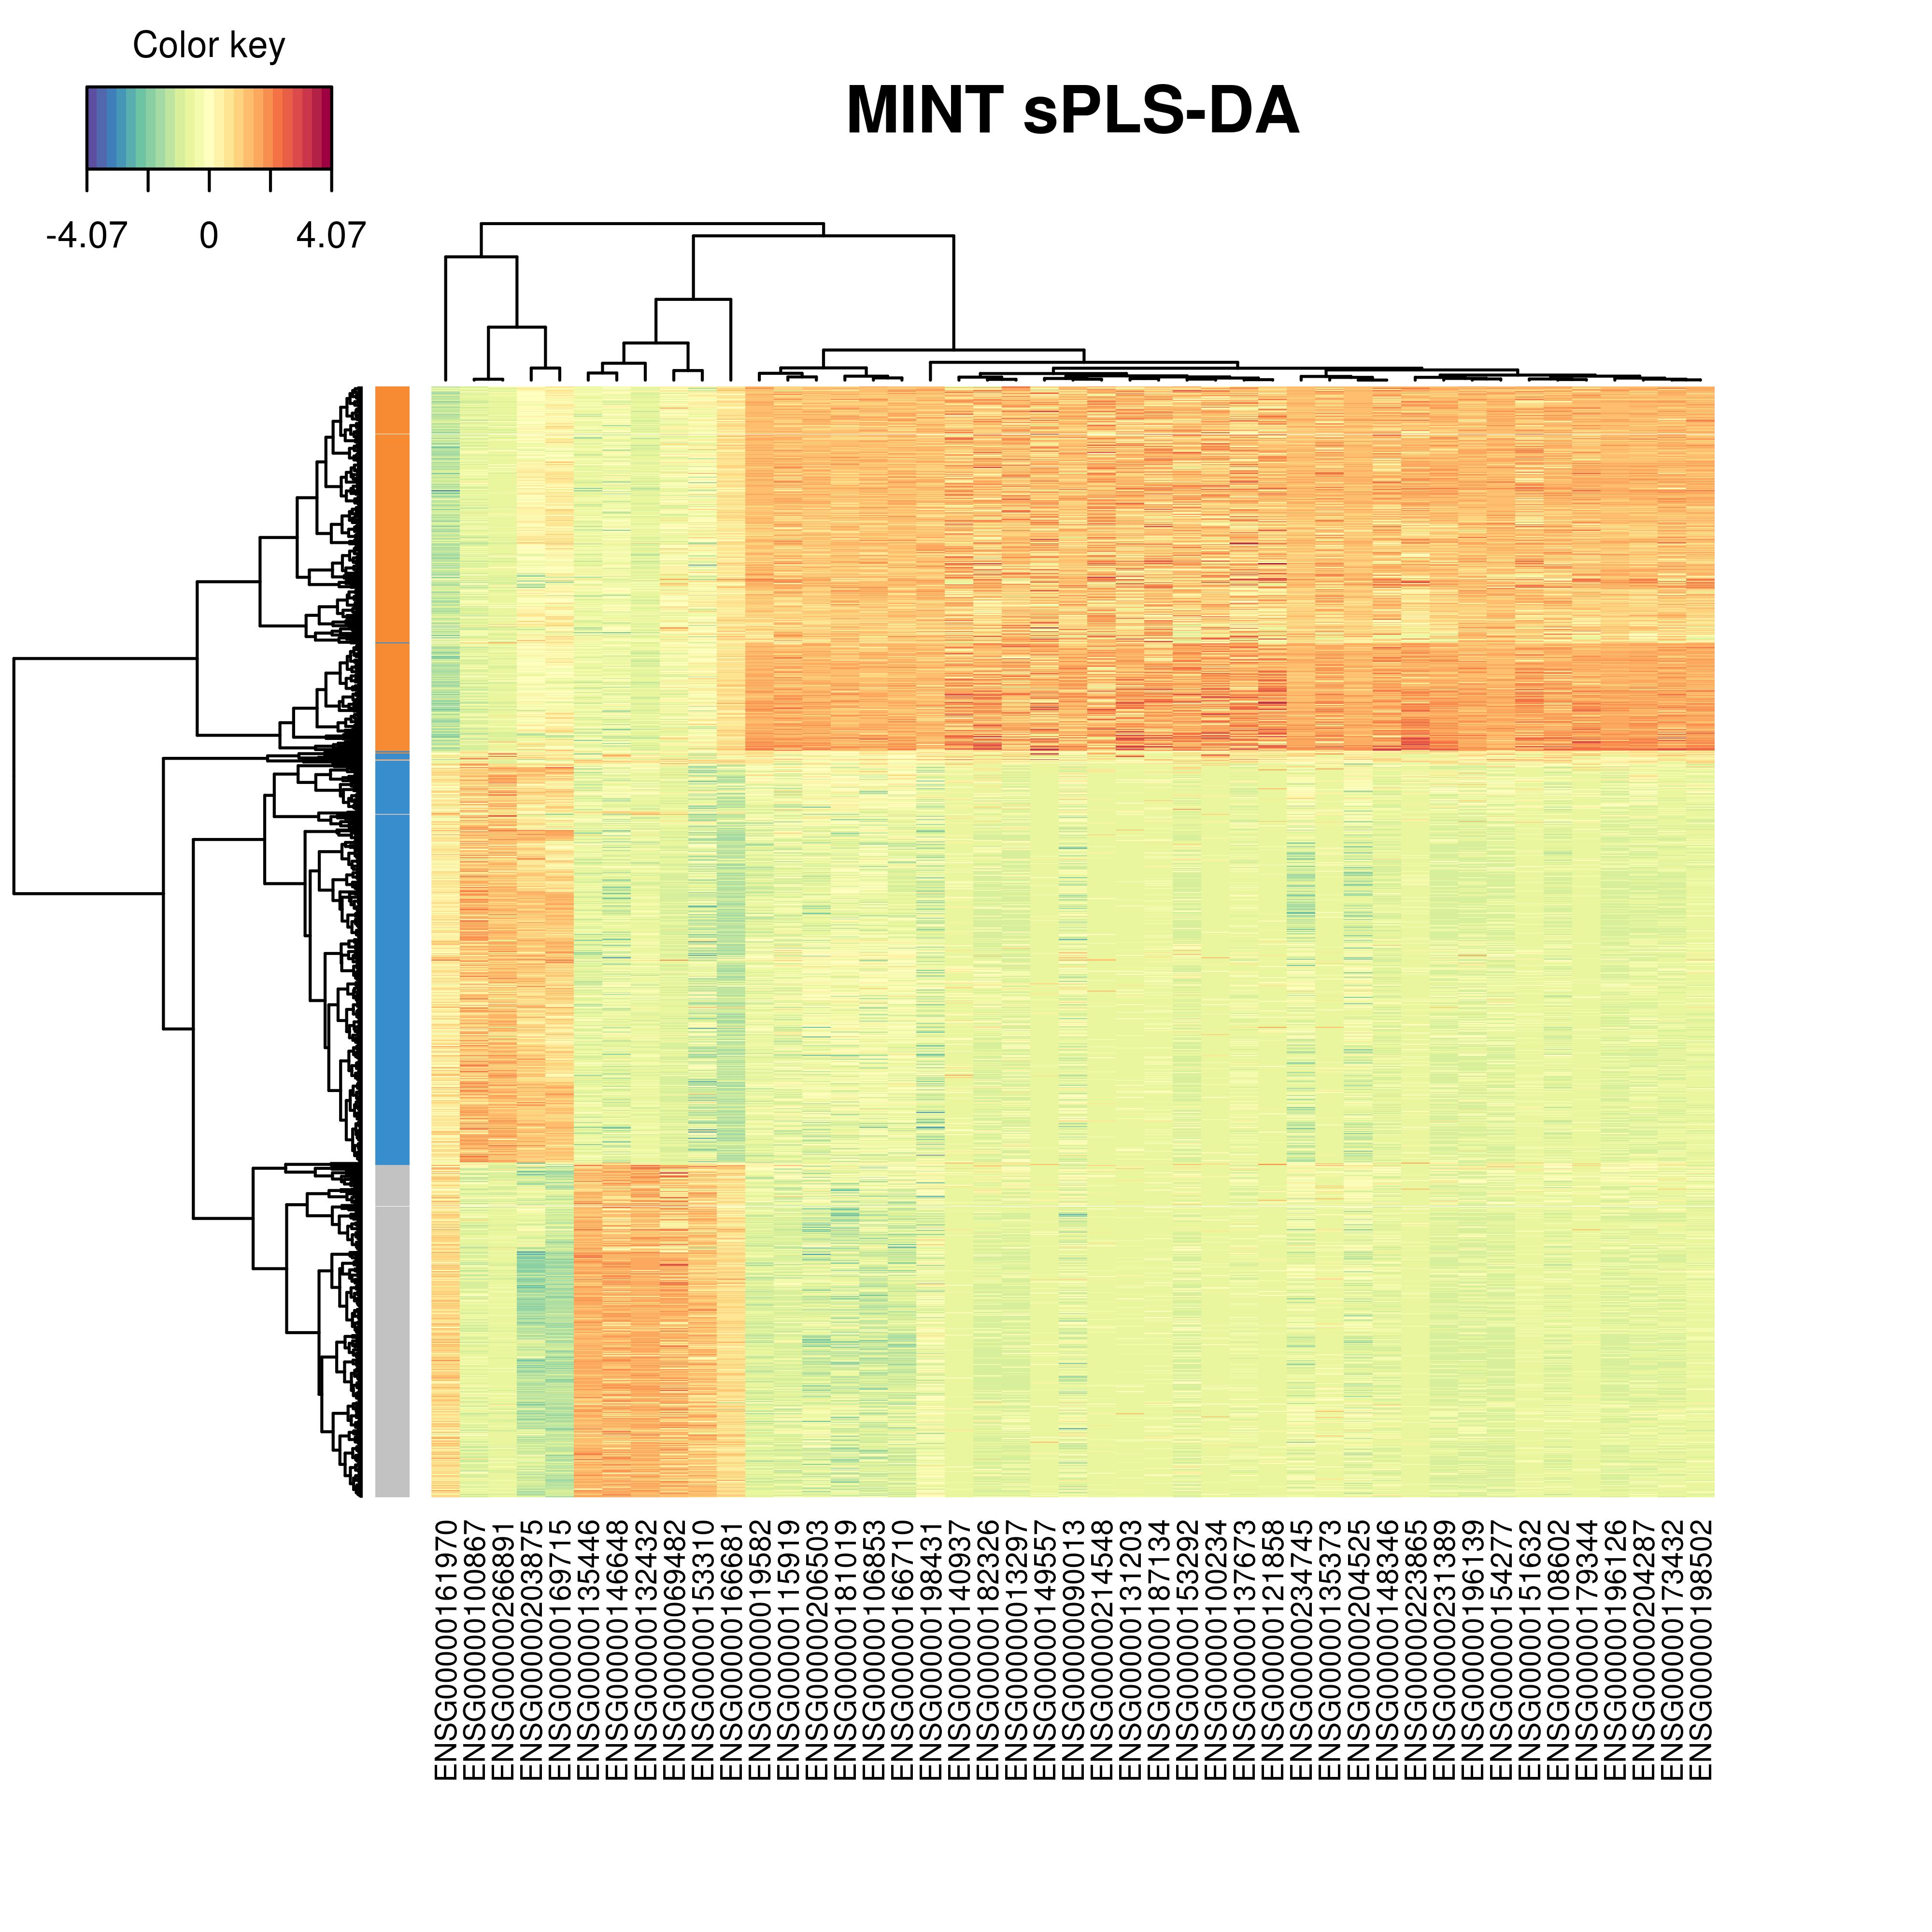
\includegraphics[width=0.8\linewidth]{heatmap} 

}

\caption{The heatmap showing the cell grouping based on the gene expression profiles.}\label{fig:2-heatmap}
\end{figure}

The heatmap shows that the cells from each cell line tend to group
together based on their gene expression profile. It can be reiterated
that the cells from the H2228 cell line show positive expression in
majority of signature genes.

\hypertarget{signature-comparison-with-bulk-assay}{%
\section{Signature Comparison with Bulk
Assay}\label{signature-comparison-with-bulk-assay}}

\hypertarget{cell-mixtures-data}{%
\subsection{Cell Mixtures Data}\label{cell-mixtures-data}}

The experimental design for CellBench data also included a cell mixture
design for a pseudo-trajectory analysis. Briefly, in this study 9 cells
were pooled from different cell types in different proportions and then
reduced to 1/9th to mimic single cells and were sequenced using CEL-seq2
protocol. A mixture of 90 cells in equal amounts was used as the control
group for a Differential Expression (DE) analysis of the pure cell lines
at the extreme of trajectories. The results available on
\href{https://github.com/LuyiTian/CellBench_data/tree/master/data}{CellBench
repository}.

\begin{figure}[ht]

{\centering 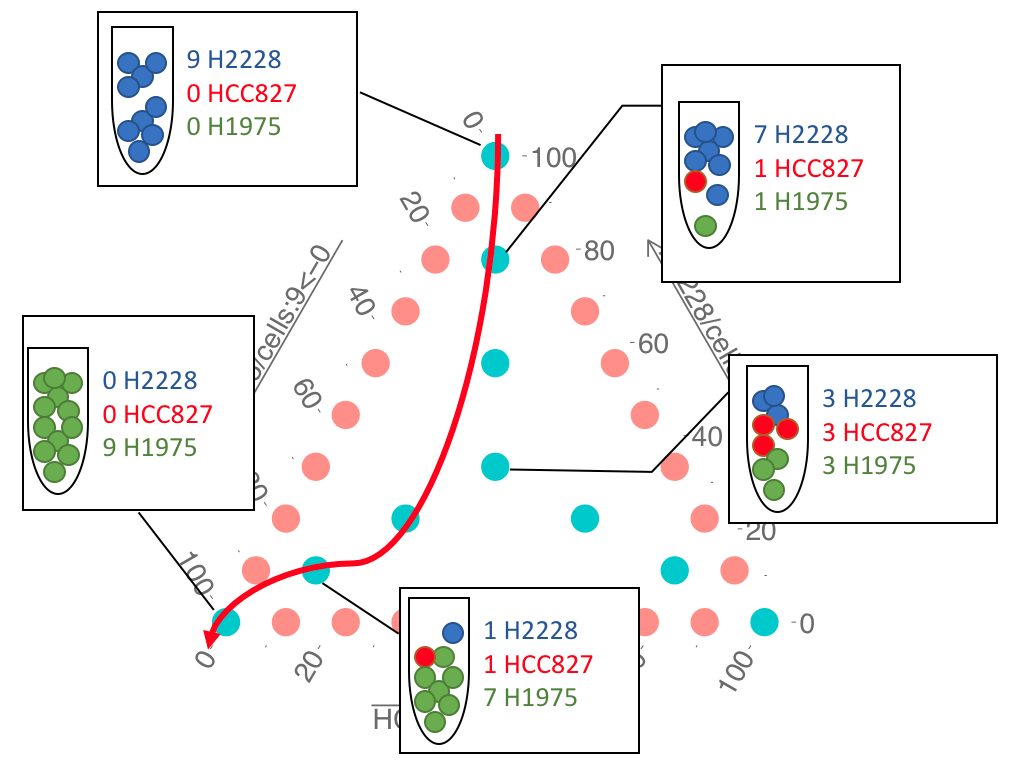
\includegraphics[width=0.55\linewidth]{figures/9cellmix} 

}

\caption{The cell mixture design. Adopted from Luyi Tian slides}\label{fig:2-cellmixdesign}
\end{figure}

We will take DE genes from the cell mixture study as reference for
comparison. The DE genes are available on CellBench respository.

\begin{Shaded}
\begin{Highlighting}[]
\CommentTok{## load directly from github}
\NormalTok{DE_URL <-}\StringTok{ 'https://tinyurl.com/DEtable-90cells'}
\KeywordTok{load}\NormalTok{(}\KeywordTok{url}\NormalTok{(DE_URL))}
\end{Highlighting}
\end{Shaded}

\hypertarget{de-genes-vs-mint-signature}{%
\subsection{DE Genes vs MINT
signature}\label{de-genes-vs-mint-signature}}

We now compare the unique signature genes from MINT sPLS-DA analysis to
the ones from cell mixture DE analysis:

\begin{Shaded}
\begin{Highlighting}[]
\CommentTok{## keep the genes present in the sPLS-DA analysis}
\NormalTok{HCC827_DEtable =}\StringTok{ }\NormalTok{HCC827_DEtable[}\KeywordTok{row.names}\NormalTok{(HCC827_DEtable) }\OperatorTok\StringTok{ }\NormalTok{list.intersect,]}
\NormalTok{H2228_DEtable =}\StringTok{ }\NormalTok{H2228_DEtable[}\KeywordTok{row.names}\NormalTok{(H2228_DEtable) }\OperatorTok\StringTok{ }\NormalTok{list.intersect,]}
\NormalTok{H1975_DEtable =}\StringTok{ }\NormalTok{H1975_DEtable[}\KeywordTok{row.names}\NormalTok{(H1975_DEtable) }\OperatorTok\StringTok{ }\NormalTok{list.intersect,]}

\CommentTok{## create a column of genes for ease of merging}
\NormalTok{HCC827_DE =}\StringTok{ }\KeywordTok{rownames_to_column}\NormalTok{(HCC827_DEtable, }\StringTok{'gene'}\NormalTok{)}
\NormalTok{H2228_DE =}\StringTok{ }\KeywordTok{rownames_to_column}\NormalTok{(H2228_DEtable, }\StringTok{'gene'}\NormalTok{)}
\NormalTok{H1975_DE =}\StringTok{ }\KeywordTok{rownames_to_column}\NormalTok{(H1975_DEtable, }\StringTok{'gene'}\NormalTok{)}

\CommentTok{## create a combined DEtable from the 3 cell lines}
\NormalTok{DEtable =}\StringTok{ }\KeywordTok{rbind}\NormalTok{(HCC827_DE,H2228_DE, H1975_DE)}
\CommentTok{## order by gene name and FDR (increasing)}
\NormalTok{DEtable =}\StringTok{ }\NormalTok{DEtable[}\KeywordTok{order}\NormalTok{(DEtable[,}\StringTok{'gene'}\NormalTok{],DEtable[,}\StringTok{'FDR'}\NormalTok{]),]}
\CommentTok{## keep the ones with FDR<0.05}
\NormalTok{DEtable =}\StringTok{ }\NormalTok{DEtable[DEtable}\OperatorTok{$}\NormalTok{FDR}\OperatorTok{<}\FloatTok{0.05}\NormalTok{,]}
\CommentTok{## remove duplicate gene names}
\NormalTok{DEtable =}\StringTok{ }\NormalTok{DEtable[}\OperatorTok{!}\KeywordTok{duplicated}\NormalTok{(DEtable}\OperatorTok{$}\NormalTok{gene),]}
\CommentTok{## overlap with MINT}
\NormalTok{DE.MINT =}\StringTok{ }\NormalTok{DEtable[(DEtable}\OperatorTok{$}\NormalTok{gene }\OperatorTok\StringTok{ }\NormalTok{MINT.Combined.vars),]}
\CommentTok{## sort in increasing FDR order}
\NormalTok{DE.MINT =}\StringTok{ }\NormalTok{DE.MINT[}\KeywordTok{order}\NormalTok{(DE.MINT}\OperatorTok{$}\NormalTok{FDR),]}
\CommentTok{## number of MINT signature genes that are differentially expressed}
\KeywordTok{dim}\NormalTok{(DE.MINT)[}\DecValTok{1}\NormalTok{]}
\end{Highlighting}
\end{Shaded}

\begin{verbatim}
## [1] 45
\end{verbatim}

\begin{Shaded}
\begin{Highlighting}[]
\CommentTok{## geometric mean of the FDR of signature}
\KeywordTok{exp}\NormalTok{(}\KeywordTok{mean}\NormalTok{(}\KeywordTok{log}\NormalTok{(DE.MINT}\OperatorTok{$}\NormalTok{FDR)))}
\end{Highlighting}
\end{Shaded}

\begin{verbatim}
## [1] 1.548651e-18
\end{verbatim}

All of signature genes identified by MINT are differentially expressed
at FDR\textless{}0.05 with geometric mean FDR of \(1.54\times10^{-18}\).

\hypertarget{session-information-1}{%
\section{Session Information}\label{session-information-1}}

\begin{Shaded}
\begin{Highlighting}[]
\CommentTok{## session information to build this vignette}
\KeywordTok{sessionInfo}\NormalTok{()}
\end{Highlighting}
\end{Shaded}

\begin{verbatim}
## R version 3.5.0 (2018-04-23)
## Platform: x86_64-apple-darwin15.6.0 (64-bit)
## Running under: macOS  10.14
## 
## Matrix products: default
## BLAS: /Library/Frameworks/R.framework/Versions/3.5/Resources/lib/libRblas.0.dylib
## LAPACK: /Library/Frameworks/R.framework/Versions/3.5/Resources/lib/libRlapack.dylib
## 
## locale:
## [1] en_AU.UTF-8/en_AU.UTF-8/en_AU.UTF-8/C/en_AU.UTF-8/en_AU.UTF-8
## 
## attached base packages:
##  [1] grid      parallel  stats4    stats     graphics  grDevices utils    
##  [8] datasets  methods   base     
## 
## other attached packages:
##  [1] tibble_1.4.2                VennDiagram_1.6.20         
##  [3] futile.logger_1.4.3         scater_1.9.24              
##  [5] scran_1.9.39                mixOmics_6.4.6             
##  [7] ggplot2_3.1.0               lattice_0.20-38            
##  [9] MASS_7.3-51.1               SingleCellExperiment_1.3.12
## [11] SummarizedExperiment_1.11.6 DelayedArray_0.7.49        
## [13] BiocParallel_1.15.15        matrixStats_0.54.0         
## [15] Biobase_2.41.2              GenomicRanges_1.33.14      
## [17] GenomeInfoDb_1.17.4         IRanges_2.15.19            
## [19] S4Vectors_0.19.24           BiocGenerics_0.27.1        
## [21] knitr_1.20                 
## 
## loaded via a namespace (and not attached):
##  [1] viridis_0.5.1             dynamicTreeCut_1.63-1    
##  [3] edgeR_3.23.7              tidyr_0.8.2              
##  [5] viridisLite_0.3.0         DelayedMatrixStats_1.3.11
##  [7] ellipse_0.4.1             assertthat_0.2.0         
##  [9] statmod_1.4.30            highr_0.7                
## [11] vipor_0.4.5               GenomeInfoDbData_1.2.0   
## [13] yaml_2.2.0                pillar_1.3.0             
## [15] backports_1.1.2           glue_1.3.0               
## [17] limma_3.37.10             digest_0.6.18            
## [19] RColorBrewer_1.1-2        XVector_0.21.4           
## [21] colorspace_1.3-2          htmltools_0.3.6          
## [23] Matrix_1.2-15             plyr_1.8.4               
## [25] pkgconfig_2.0.2           bookdown_0.7             
## [27] zlibbioc_1.27.0           purrr_0.2.5              
## [29] corpcor_1.6.9             scales_1.0.0             
## [31] HDF5Array_1.9.19          RSpectra_0.13-1          
## [33] withr_2.1.2               lazyeval_0.2.1           
## [35] magrittr_1.5              crayon_1.3.4             
## [37] evaluate_0.12             beeswarm_0.2.3           
## [39] tools_3.5.0               formatR_1.5              
## [41] stringr_1.3.1             Rhdf5lib_1.3.3           
## [43] munsell_0.5.0             locfit_1.5-9.1           
## [45] lambda.r_1.2.3            bindrcpp_0.2.2           
## [47] compiler_3.5.0            rlang_0.3.0.1            
## [49] rhdf5_2.25.11             RCurl_1.95-4.11          
## [51] BiocNeighbors_0.99.22     rstudioapi_0.8           
## [53] igraph_1.2.2              labeling_0.3             
## [55] bitops_1.0-6              rmarkdown_1.10           
## [57] gtable_0.2.0              codetools_0.2-15         
## [59] rARPACK_0.11-0            reshape2_1.4.3           
## [61] R6_2.3.0                  gridExtra_2.3            
## [63] dplyr_0.7.8               bindr_0.1.1              
## [65] rprojroot_1.3-2           futile.options_1.0.1     
## [67] ggbeeswarm_0.6.0          stringi_1.2.4            
## [69] Rcpp_1.0.0                tidyselect_0.2.5         
## [71] xfun_0.4
\end{verbatim}

\bibliography{packages.bib,citations.bib}


\end{document}
